%Text Books : \cite{kreyszig}
%Module 1:
%Examples, Completeness proofs, Completion of Metric Spaces, Vector Space, Normed Space, Banach space, Further Properties of Normed Spaces, Finite Dimensional Normed spaces and Subspaces, Compactness and Finite Dimension
%(Chapter 1 - Sections 1.5, 1.6; Chapter 2 - Sections 2.1 to 2.5)
%Module 2:
%Linear Operators, Bounded and Continuous Linear Operators, Linear Functionals, Linear Operators and Functionals on Finite dimensional spaces, Normed spaces of operators, Dual space
%(Chapter 2 - Section 2.6 to 2.10)
%Module 3:
%Inner Product Space, Hilbert space, Further properties of Inner Product Space, Orthogonal Complements and Direct Sums, Orthonormal sets and sequences, Series related to Orthonormal sequences and sets, Total Orthonormal sets and sequences, Representation of Functionals on Hilbert Spaces
%(Chapter 3 - Sections 3.1 to 3.6, 3.8)
%Module 4:
%Hilbert-Adjoint Operator, Self-Adjoint, Unitary and Normal Operators, Zorn's lemma, Hahn- Banach theorem, Hahn-Banach theorem for Complex Vector Spaces and Normed Spaces, Adjoint Operators
%(Chapter 3 - Sections 3.9, 3.10; Chapter 4 - Sections 4.1 to 4.3, 4.5)

%Module 1 - \cite{kreyszig} 1
%Module 2 - \cite{kreyszig} 2
%Module 3 - \cite{kreyszig} 3
%Module 4 - \cite{kreyszig} 3, 4

%Module 1 - Erwin Kreyszig 1.5-1.6, 2.1-2.5
%\chapter 1
{\Large Module 1 - Banach Space}
\section{Metric Spaces}
The following are a few metric spaces and their distance functions,
\begin{enumerate}
	\item $\mathbb{R}, d(x,y) = |x -y|$
	\item $\mathbb{R}^2, d(x,y) = \left( |\xi_1-\eta_1|^2 + |\xi_2 - \eta_2|^2 \right)^\frac{1}{2} $ where $x = (\xi_1,\xi_2)$
	\item $\mathbb{R}^3, d(x,y) = \left( |\xi_1-\eta_1|^2 + |\xi_2 - \eta_2|^2 + |\xi_3-\eta_3|^2 \right)^\frac{1}{2} $ where $x = (\xi_1,\xi_2,\xi_3)$
	\item Euclidean space, $\displaystyle \mathbb{R}^n, d(x,y) = \left( \sum_{j=1}^n |\xi_j - \eta_j|^2 \right)^\frac{1}{2}$ where $x = (\xi_1,\xi_2,\dots,\xi_n)$
	\item $\mathbb{C}, d(x,y) = |x - y|$ where $x = a+ib$ and $|x| = (a^2+b^2)^\frac{1}{2}$
	\item Unitary space, $\displaystyle \mathbb{C}^n, d(x,y) =  \left( \sum_{j=1}^n |\xi_j - \eta_j|^2 \right)^\frac{1}{2}$ where  $x = (\xi_1,\xi_2)$ and $\xi_j \in \mathbb{C}$.
	\item $\displaystyle C[a,b], d(x,y) = \max_{t \in [a,b]} \left\{ |x(t)-y(t)| \right\}$ where $x$ is a continuous, complex-valued function defined on closed interval $[a,b] \subset \mathbb{R}$.
	\item $\displaystyle B(A), d(x,y) = \sup_{t \in A} \left\{ |x(t)-y(t)| \right\}$ where $x$ is a bounded, complex-valued function defined on $A \subset \mathbb{R}$
	\item $\displaystyle l^p, d(x,y) = \left( \sum_{j = 1}^\infty |\xi_j - \eta_j|^p \right)^\frac{1}{p}$ where $x = \sequence{\xi_j}$ and $\displaystyle \sum_{j=1}^\infty |\xi_j|^p < \infty$. That is, set of all sequences such that the $p$th power series is convergent.
	\item $\displaystyle l^\infty, d(x,y) = \sup_{j \in \mathbb{N}} \{ |\xi_j - \eta_j| \} $ where $x = \sequence{\xi_j}$ and $|\xi_j| \le c$. That is, $l^\infty$ is the space of all bounded sequences of complex numbers.
	\item $\displaystyle c, d(x,y) = \sup_{j \in \mathbb{N}} \{ |\xi_j - \eta_j| \}$ where $\sequence{\xi_j} = \xi_1,\xi_2,\dots$ is the space of all convergent sequences of complex numbers.
	\item $\displaystyle s, d(x,y) = \sum_{j = 1}^\infty \frac{1}{2^j} \frac{|\xi_j - \eta_j|}{1+|\xi_j-\eta_j|}$ where $x = \sequence{\xi_j} = \xi_1,\xi_2,\dots$ is the space of all sequence of complex numbers.
\end{enumerate}
Clearly, $l^p \subset l^\infty \subset s$.
But, $B(A),C[a,b]$ are non-comparable since there exists discontinuous, bounded functions and continuous, unbounded functions.

\begin{definition}[conjugate exponents]
	Real numbers $p,q$ are conjugates, if $p>1,q>1$ and $\frac{1}{p}+\frac{1}{q} = 1$.
\end{definition}
Note : if $p,q$ are conjugates, then $p+q=pq$ and $(p-1)(q-1) = 1$.
Also if $u = t^{p-1}$, then $t = u^{q-1}$.

\begin{theorem}[H\"older\footnote{O.H\"older} Inequality for sums]
	Let $p,q$ be conjugates and $(\xi_j), (\eta_j)$ be two complex sequences. $(\xi_j) \in l^p$ and $(\eta_j) \in l^q$.
	Then
	\begin{equation}
		\sum_{j=1}^\infty |\xi_j\eta_j| \le \left( \sum_{j=1}^\infty |\xi_j|^p \right)^\frac{1}{p} \quad \left( \sum_{j=1}^\infty |\eta_j|^q \right)^\frac{1}{q}
	\end{equation}
\end{theorem}
\begin{corollary}[Cauchy-Schwarz Inequality]
	When $p=2$, we have its conjugate $q=2$.
	Then H\"older inequality reduces to the following
	\begin{equation}
		\sum_{j=1}^\infty |\xi_j\eta_j| \le \left( \sum_{j=1}^\infty |\xi_j|^2 \right)^\frac{1}{2} \quad \left( \sum_{j=1}^\infty |\eta_j|^2 \right)^\frac{1}{2}
	\end{equation}

\end{corollary}
\begin{theorem}[Minkowski\footnote{H. Minkowski} Inequality]
	Let $p,q$ be conjugates and $(\xi_j), (\eta_j)$ be two complex sequences in $l^p$.
	Then
	\begin{equation}
		\left( \sum_{j=1}^\infty |\xi_j + \eta_j|^p \right)^\frac{1}{p} \le \left( \sum_{j=1}^\infty |\xi_j|^p \right)^\frac{1}{p} + \left( \sum_{j=1}^\infty |\eta_j|^q \right)^\frac{1}{q}
	\end{equation}
\end{theorem}
\subsection{A few more Concepts}
\begin{description}
	\item[product of metric spaces]
		Let $(X_1,d_1),(X_2,d_2)$ be two metric spaces.
		Let $x,y \in X_1 \times X_2$ where $x = (\xi_1,\xi_2 )$ and $y = (\eta_1,\eta_2)$.
		Then, $X_1 \times X_2$ is a metric space with following metrics,
		\begin{enumerate}
			\item $\displaystyle d(x,y) = d_1\left(\xi_1,\eta_1\right) + d_2\left(\xi_2,\eta_2\right)$
			\item $\displaystyle d(x,y) = \left( d_1\left( \xi_1,\eta_1 \right)^2 + d_2\left(\xi_2,\eta_2\right)^2 \right)^\frac{1}{2}$
			\item $\displaystyle d(x,y) = \max \{ d_1 \left(\xi_1,\eta_1\right) , d_2\left(\xi_2,\eta_2\right) \}$
		\end{enumerate}
	\item[separable] A space is separable if it has a countable, dense subset.\\
		Examples : $l^\infty$ is not separable. But, $l^p$ spaces are separable $(1 \le p <\infty)$. $\mathbb{R},\mathbb{C}$ are separable. $B[a,b]$ not seprable.
\end{description}
\subsection{Exercises}
\begin{enumerate}
	\item Find a sequence $\sequence{\xi_j}$ which converges to $0$ but does not belong to any $l^p$ space. $(1 \le p < \infty)$.
	\item Find a sequence $\sequence{\xi_j}$ which belong to $l^p$ space with $p>1$, but not in $l^1$.
\end{enumerate}
\setcounter{subsection}{4}
\subsection{Completeness}
Convergent sequences in a metric space are Cauchy sequences. But, Cauchy sequences are not necessarily convergent.
\begin{definition}[complete]
	A metric space is complete if every Cauchy sequence in it is convergent.
\end{definition}
\begin{theorem}
	$\mathbb{R}$ is complete.
\end{theorem}
\begin{proof}
	Let $\sequence{\xi_n}$ be a Cauchy sequence in $\mathbb{R}$.
	Let $M_0 > 0$.
	Then, there exists $N \in \mathbb{N}$ such that $\forall n,m > N,\ d(x_n,x_m) < M_0$.
	Let $M = \max \{M_0,M_1,\dots,M_N \}$ where $\forall n \le N,\ |\xi_j| < M_j$.
	Then $\sequence{\xi_n}$ is bounded by $M$.\\

	By Bolzano Weierstrass\dag\footnote{
		Every sequence has a monotone subsequence.
		And by monotone converges theorem, every monotone bounded sequence has a convergent subsequence.} 
	theorem, every bounded sequence in $\mathbb{R}^n$ has a convergent subsequence.
	Let $x \in \mathbb{R}$ be the limit of a convergent subsequence $\sequence{\xi_{n_k}}$ of $\sequence{\xi_n}$.
	Then $\xi_n \to x$ since $\sequence{\xi_n}$ is a Cauchy sequence.
\end{proof}

\begin{theorem}
	$\mathbb{C}$ is complete.
\end{theorem}
\begin{proof}
	Let $\sequence{\xi_n}$ be a Cauchy sequence in $\mathbb{C}$.
	Then the real, imaginary parts of $\xi_n$ are a Cauchy sequences in $\mathbb{R}$.
	We know that $\mathbb{R}$ is complete.
	Let $\Re(\xi_n) \to a$ and $\Im(\xi_n) \to b$.
	Then $\xi_n \to a+ib$ since $\sequence{\xi_n}$ is a Cauchy sequence.
\end{proof}

\begin{theorem}
	Finite dimensional Euclidean space, $\mathbb{R}^n$ is complete.
\end{theorem}
\begin{proof}
	Let $\sequence{x_k}$ be Cauchy sequence in $\mathbb{R}^n$.
	Let $\varepsilon > 0$.
	There exists $N \in \mathbb{N}$ such that $\forall m,r > N,\ d(x_m,x_r) < \varepsilon$.
	Let $x_m = (\xi_{1,m},\xi_{2,m},\dots,\xi_{n,m})$ and $x_r = (\xi_{1,r},\xi_{2,r},\dots,\xi_{n,r})$.
	\begin{align*}
		d(x_m,x_r) = \left( \sum_{j=1}^n |\xi_{j,m} - \xi_{j,r}|^2 \right)^\frac{1}{2} & <  \varepsilon\\
		\implies \sum_{j=1}^n |\xi_{j,m} - \xi_{j,r}|^2 & <  \varepsilon^2 \\
		\implies |\xi_{j,m} - \xi_{j,r}| & < \varepsilon^2,\ j = 1,2,\dots,n
	\end{align*}
	Therefore, $\sequence{\xi_{j,k}}$'s are Cauchy sequences in $\mathbb{R}$ for $j = 1,2,\dots,n$.
	Since $\mathbb{R}$ is convergent, $\xi_{j,k} \to \xi_j$ for each $j$.
	Let $x = (\xi_1,\xi_2,\dots,\xi_n)$.
	Let $\varepsilon > 0$.
	Then there exists $N_j \in \mathbb{N}$ such that $\forall m > N,\ |\xi_{j,m} - \xi_j|  < \frac{\varepsilon}{n} $.
	Let $N = \max \{ N_1,N_2,\dots,N_n\}$.
	Then $\forall m > N$,
	\[ d(x_m,x) = \left( \sum_{j=1}^n | \xi_{j,m} - \xi_j|^2 \right)^\frac{1}{2} = \left( \sum_{j=1}^n \frac{\varepsilon^2}{n^2} \right)^\frac{1}{2} = \frac{\varepsilon}{\sqrt{n}} < \varepsilon \]
	Therefore, $\sequence{x_n}$ converges to $x$ in $\mathbb{R}^n$.
\end{proof}

\begin{theorem}
	Finite dimensional Unitary space, $\mathbb{C}^n$ is complete.
\end{theorem}
\begin{proof}
	Same proof as above.
\end{proof}

\begin{theorem}
	The complex sequence space of all bounded sequences, $l^\infty$ is complete.
\end{theorem}
\begin{proof}
	Let $\sequence{x_k}$ be a Cauchy sequence in $l^\infty$ where $x_k = \xi_{k,1},\ \xi_{k,2},\ \dots$ are bounded sequences in $\mathbb{C}$ for each $k$.\\
	\textbf{Step 1 : Construct $x$}\\
	Let $\varepsilon > 0$.
	Then there exists $N \in \mathbb{N}$ such that $\forall m,n > N$,
	\[ d(x_m,x_n) = \sup_{k \in \mathbb{N}} \left\{ \left|\xi_{m,k} - \xi_{n,k} \right| \right\} < \varepsilon \]
	From the metric, we have $\sequence{\xi_{j,k}}$'s are Cauchy sequences in $\mathbb{C}$ for each $k$.
	\begin{figure}
		\[ \begin{matrix}
			x_1 = & \xi_{1,1} & \xi_{1,2} & \xi_{1,3} & \dots \\
			x_2 = & \xi_{2,1} & \xi_{2,2} & \xi_{2,3} & \dots \\
			x_3 = & \xi_{3,1} & \xi_{3,2} & \xi_{3,3} & \dots \\
			\vdots & \vdots & \vdots & \vdots & \vdots \\
			x = & \xi_1 & \xi_2 & \xi_3 & \dots 
		\end{matrix} \]
		\caption{Construction of limit in Sequence spaces}
	\end{figure}
	Thus, $\xi_{j,k} \to \xi_k \in \mathbb{C}$.
	Let $x = \xi_1,\ \xi_2,\ \dots $.
	Now we need to prove that $x_k \to x$ and $x \in l^\infty$.\\
	\textbf{Step 2 : $x \in l^\infty$}\\
	We have, $x_j \in l^\infty \implies |\xi_{m,j}| < c_j, \ \forall m \in \mathbb{N} $.
	Therefore,
	\[ |\xi_j| \le |\xi_j-\xi_{m,j}| + |\xi_{m,j}| \le \varepsilon + c_j, \quad \forall j \in \mathbb{N} \]
	Thus, $x \in l^\infty$.\\
	\textbf{Step 3 : $x_n \to x$}\\
	Since $|\xi_{m,j}-\xi_j| < \varepsilon$ for $m \in \mathbb{N}$,
	\[ d(x_m,x) = \sup_{j \in \mathbb{N}} |\xi_{m,j} - \xi_j| \le \varepsilon \]
\end{proof}

\begin{theorem}
	The complex sequence space of all convergent sequences, $c$ is complete
\end{theorem}
\begin{proof}
	Since every convergent sequence is bounded, $c \subset l^\infty$.
	And the sequence space $c$ is complete if $c$ is a closed subset of the complete space $l^\infty$.
	Therefore, it is sufficient to show that $c = \closure{c}$\\

	Let $x = \sequence{\xi_k} \in \closure{c}$.	
	Then there exists a convergent sequence $\sequence{x_k} = \sequence{\xi_{k,j}}$ in $c$ converging to $x$.
	That is, $\xi_{k,j} \to \xi_j$.\\

	Let $\varepsilon > 0$.
	Then there exists $N \in \mathbb{N}$ such that $\forall n \ge N$ and $\forall j,k \in \mathbb{N}$, we have $\displaystyle d(x_N,x) = \sup_{r \in \mathbb{N}} \{ |\xi_{n,r} - \xi_r| \} < \frac{\varepsilon}{3}$.
	Therefore,
	\begin{equation}
		|\xi_{N,j} - \xi_j| < \frac{\varepsilon}{3} \text{ and } |\xi_{N,k} - \xi_k| < \frac{\varepsilon}{3} 
	\end{equation}
	Every convergent sequence in complete metric space $l^\infty$ is also a Cauchy sequence.
	Since $x_N = \sequence{\xi_{N,k}}$ is a Cauchy sequence, there exists $N_1 \in \mathbb{N}$ and $\forall j,k \ge N_1$,
	\begin{equation}
		|\xi_{N,j} - \xi_{N,k}| < \frac{\varepsilon}{3}
	\end{equation}
	Therefore,
	\[ |\xi_j - \xi_k| \le |\xi_j - \xi_{N,j}| + |\xi_{N,j}-\xi_{N,k}| + |\xi_{N,k} - \xi_k| \le \frac{\varepsilon}{3} + \frac{\varepsilon}{3} + \frac{\varepsilon}{3} = \varepsilon \]
	Clearly, $x = \sequence{\xi_k}$ is a Cauchy sequence in $l^\infty$.
	And since $l^\infty$ is complete, every Cauchy sequence in $l^\infty$ is convergent.
	Therefore, $x$ is a convergent sequence and $x \in c$.
	Thus, $c = \closure{c}$ and the induced\dag\footnote{
		Let $(X,d)$ be a complete metric space.
		And $Y$ is a closed subset of $X$.
		Then the induced metric space $(Y,d_{|_Y})$ is complete.}
	metric space $c$ is complete.
\end{proof}

\begin{theorem}
	For any $p \ge 1$, the sequence space $l^p$ is complete.
\end{theorem}
\begin{proof}
	Let $\sequence{x_k}$ be a Cauchy sequence $l^p$ where $x_k = \sequence{\xi_{k,j}}$ and
	\[ \sum_{j = 1}^\infty \left| \xi_{k,j} \right|^p < \infty,\ \forall k \in \mathbb{N} \]
	Since $\sequence{x_k}$ is a Cauchy sequence, for $\varepsilon > 0$ there exists $N \in \mathbb{N}$ such that
	\begin{equation}
		\label{equ:lpcauchy}
		d(x_m,x_n) = \left( \sum_{j=1}^\infty |\xi_{m,j} - \xi_{n,j}|^p \right) ^\frac{1}{p} < \varepsilon,\quad \forall m,n > N \text{ since } x_k \in l^p
	\end{equation}
	Thus, $\forall m,n > N,\ |\xi_{m,j} - \xi_{n,j}| < \varepsilon$ for each $j$.

	\textbf{Step 1 : Construction of $x$}\\
	Define $x = \sequence{\xi_j}$ where $\xi_j$ is an accumulation point of $\sequence{\xi_{k,j}}$.\\% Then $\xi_{k,j} \to \xi_j$ OR $x_k \to x$. \\

	\textbf{Step 2 : $x \in l^p$}\\
	Let $j > N$.
	Then, $\sequence{\xi_{k,j}}$ is a Cauchy sequence of complex numbers.
	Then, $\xi_{k,j} \to \xi_j$.
	Applying limit $n \to \infty$ on equation \ref{equ:lpcauchy}, we get
	\begin{align*}
		\left( \sum_{j=1}^\infty |\xi_{m,j} - \xi_j|^p \right) ^\frac{1}{p} & < \varepsilon,\quad \forall m > N \\
		\implies \sum_{j=1}^\infty |\xi_{m,j} - \xi_j|^p  & < \varepsilon^p
	\end{align*}
	Let $m > N$. Then $x_m - x \in l^p$. By Minkowski inequality, we have
	\begin{equation}
		\sum_{j=1}^\infty |\xi_j|^p  \le \sum_{j=1}^\infty |\xi_{m,j}-\xi_j|^p + \sum_{j=1}^\infty |\xi_{m,j}|^p  < \infty
	\end{equation}
	Thus, $x \in l^p$. \\
	\textbf{Step 3: $x_m \to x$}\\
	Since $\displaystyle \sum_{j=1}^\infty |\xi_{m,j} - \xi_j|^p < \varepsilon^p$, we have $\xi_{k,j} \to \xi_j$.
	Therefore, $x_m \to x$.
\end{proof}

\begin{theorem}
	The function space of all continuous functions defined on closed interval $[a,b]$, $C[a,b]$ is complete.
\end{theorem}
\begin{proof}
	Let $\sequence{x_k}$ be a Cauchy sequence in $C[a,b]$.\\
	Let $\varepsilon > 0$.
	Then there exists $N \in \mathbb{N}$ such that $m,n > N$, 
	\[ d(x_m,x_n) = \max_{t \in [a,b]} \left\{ x_m(t) - x_n(t) \right\} < \varepsilon \]
	Thus, for each $t \in [a,b]$, sequence $\sequence{x_k(t)}$'s are Cauchy sequences.
	We know that $\mathbb{C}$ is complete.
	Thus every Cauchy sequence in $\mathbb{C}$ is convergent.\\

	Define $x : [a,b] \to \mathbb{C}$ defined by $x(t) = $ the limit of the sequence $\sequence{x_k(t)}$.
	As $n \to \infty$, $d(x_m,x_n) \to d(x_m,x)$ and for any $m > N$, $d(x_m,x) < \varepsilon$ uniformly.
	It is evident from the construction that, the convergence $x_k(t) \to x(t)$ is uniform.\\

	Since the function $x_k$'s are continuous and the convergence is uniform, the limit function $x$ is also continuous.
	Therefore $x \in C[a,b]$.
\end{proof}

\begin{definition}[uniform metric]
	Let $(X,d)$ be a metric space in which every convergence $x_k \to x$ is uniform.
	Then the metric $d$ is a uniform metric.
\end{definition}
For example, the metric of $C[a,b]$ is a uniform metric.

\subsubsection{A few examples of incomplete metric spaces}
The following metric spaces are not complete,
\begin{enumerate}
	\item The space of rational numbers, $\mathbb{Q}$ with usual metric $d(x,y) = |x-y|$ is not complete since the rational approximations of $\pi$ is sequence in $\mathbb{Q}$ which doesn't converge in $\mathbb{Q}$.
		\[ 3,\ 3.1,\ 3.14,\ 3.141,\ \dots \to \pi \notin \mathbb{Q} \]
	\item The space of polynomial functions with metric $d(x,y) = \sup \{ x(t) - y(t)|$ is not complete since taylor approximations of $\sin x$ is a sequence of polynomial funcitons which doesn't converge to a polynomial function.
		\[ x,\ x+\frac{-x^3}{3!},\ x+\frac{-x^3}{3!}+\frac{x^5}{5!},\ \dots \to \sin x \notin p \]
	\item The space of continuous function on unit interval $[0,1]$ with a different\dag\footnote{Area under the graph of difference function is well-defined for integrable functions.} metric 
		\[ d(x,y) = \int_0^1 \left| x(t)-y(t) \right| \ dt \]
		is not complete since $\sequence{x_k}$ where $x_k : [0,1] \to \mathbb{R}$ is defined by
		\[ x_k(t) = \begin{cases} 0 & t \in \left[0,\frac{1}{2}\right) \\
			(t-\frac{1}{2})k & t \in \left[\frac{1}{2},\frac{1}{2}+\frac{1}{k}\right) \\
		1 & t \in \left[\frac{1}{2}+\frac{1}{k},1\right] \end{cases} \]
		doesn't converge to a continuous polynomial function.
\end{enumerate}
\subsection{Completion of Metric Space}
Let $Y$ be an incomplete metric space.
Completion of $Y$ is a construction of a complete metric space $X$ in which $Y$ is dense.\\

For example, $\mathbb{Q}$ is not complete. However, $\mathbb{R}$ is a complete metric space in which $\mathbb{Q}$ is complete. Therefore, $\mathbb{R}$ is a completion of $\mathbb{Q}$.

\begin{definition}[Isometry]
	Isometric functions are distance preserving functions.
	And two metric spaces are isometric if there exists a bijective isometry between them.
\end{definition}

For example, function $f : X \to Y$ is an isometry if
\[ \forall x,y \in X,\quad \hat{d}(f(x),f(y)) = d(x,y) \]
where $d, \hat{d}$ are metrics in $X,Y$ respectively.
And if  $f$ is a bijection, then $X,Y$ are isometric space.\\

\begin{commentary}
	Two metric spaces are isometric is another way of saying that the spaces are identical (same) from metric point of view.
\end{commentary}

\begin{theorem}[completion]
	Let $(X,d)$ be a metric space.
	Then, there exists a complete metric space, $(\hat{X},\hat{d})$ such that it has a dense subspace $W$ which is isometric with $X$.
	And $\hat{X}$ is unique upto isomerties.
\end{theorem}
\begin{commentary}
	In other words, for any metric space $X$ there exists a unique complete metric space, $\hat{X}$ in which $X$ is dense.
\end{commentary}
\begin{proof}
	\textbf{Step 1 : Construction of $(\hat{X},\hat{d})$}\\
	Let $(X,d)$ be a metric space.
	Let $C$ be the set of all Cauchy sequence in $X$.
	Define relation $\sequence{x_k} \sim \sequence{y_k}$ if and only if $\displaystyle \lim_{k \to \infty} d(x_k,y_k) = 0$.
	This is an equivalence relation.(proof not required)

	\begin{commentary}
		{\footnotesize
		\begin{enumerate}
			\item Reflexive - $\displaystyle \hat{x} \sim \hat{x}$ since $\lim_{k \to \infty} d(x_k,x_k) = 0$. 
			\item Symmetric -  $\displaystyle \hat{x} \sim \hat{y} \implies \lim_{k \to \infty} d(x_k,y_k) = \lim_{k \to \infty} d(y_k,x_k) \implies \hat{y} \sim \hat{x}$.
		\item Transitive - Suppose, $\hat{x} \sim \hat{y}$ and $\hat{y} \sim \hat{z}$.\\
		$\displaystyle \hat{x} \sim \hat{y} \implies \hat{d}(\hat{x},\hat{y}) = \lim_{k \to \infty} d(x_k,y_k) = 0$, $\displaystyle \hat{y} \sim \hat{z} \implies \hat{d}(\hat{y},\hat{z}) = \lim_{k \to \infty} d(y_k,z_k) = 0$.\\
		Then $\displaystyle \hat{d}(\hat{x},\hat{z}) = \lim_{k \to \infty} d(x_n,z_n) \le \lim_{k \to \infty} d(x_n,y_n) + d(y_n,z_n) = \hat{d}(\hat{x},\hat{y}) + \hat{d}(\hat{y},\hat{z}) = 0$.\\
		Therefore $\hat{x} \sim \hat{z}$.
		\end{enumerate}
		}
	\end{commentary}

	Let $\hat{X}$ be the set of all equivalent classes in $C$.
	Define $\hat{d} : \hat{X} \times \hat{X} \to \mathbb{R}$ given by  $\displaystyle \hat{d}(\hat{x},\hat{y}) = \lim_{k \to \infty} d(x_k,y_k)$ where the Cauchy sequences $\sequence{x_k} \in \hat{x}$ and $\sequence{y_k} \in \hat{y}$.
	Then $\hat{d}$ is metric in $\hat{X}$.
	\begin{enumerate}
		\item $\hat{d}$ is well-defined\\
			Suppose $\sequence{x_k},\sequence{x_k'} \in \hat{x}$ and $\sequence{y_k},\sequence{y_k'} \in \hat{y}$.
			Then $\sequence{x_k} \sim \sequence{x_k'}$ and $\sequence{y_k} \sim \sequence{y_k'}$.
			In other words, $\displaystyle \lim_{k \to \infty} d(x_k,x_k') = 0$ and $\displaystyle \lim_{k \to \infty} d(y_k,y_k') = 0$.\\

			By triangular inequality, we have
			\[ d(x_k,y_k) \le d(x_k,x_k') + d(x_k',y_k') + d(y_k',y_k) \]
			\[ \implies d(x_k,y_k) - d(x_k',y_k') \le d(x_k,x_k') + d(y_k,y_k') \]
			Similarly,
			\[ d(x_k',y_k') \le d(x_k',x_k) + d(x_k,y_k) + d(y_k,y_k') \]
			\[ \implies d(x_k',y_k') - d(x_k,y_k) \le d(x_k,x_k') + d(y_k,y_k') \]
			Therefore, 
			\[ | d(x_k,y_k) - d(x_k',y_k')| \le d(x_k,x_k') + d(y_k,y_k')  \]
			Apply the limit $k \to \infty$ on either sides, we get
			\[ \lim_{k\to \infty} |d(x_k,y_k)-d(x_k',y_k')| \le \lim_{k \to \infty} d(x_k,x_k') + \lim_{k \to \infty} d(y_k,y_k') = 0 \]
			Thus, $\hat{d}(\hat{x},\hat{y})$ depends only on the equivalent class $\hat{x},\hat{y}$ to which $x_k,y_k$ belongs and is independent of the representative from these equivalent classes.
			Therefore, $\hat{d} : \hat{X} \times \hat{X} \to \mathbb{R}$ is well-defined.
		\item $\hat{d}(\hat{x},\hat{y}) = 0 \iff \hat{x} = \hat{y}$
			\[ \hat{d}(\hat{x},\hat{y}) = 0 \iff \forall \sequence{x_k} \in \hat{x}, \forall \sequence{y_k} \in \hat{y},\ \lim_{k \to \infty} d(x_k,y_k) = 0 \iff \sequence{x_k} \sim \sequence{y_k} \]
		\item $\hat{d}(\hat{x},\hat{y}) = \hat{d}(\hat{y},\hat{x})$ is trivial since $d(x_k,y_k) = d(y_k,x_k)$.
		\item $\hat{d}(\hat{x},\hat{y}) \le \hat{d}(\hat{x},\hat{z}) + \hat{d}(\hat{z},\hat{y})$\\

			Let $\sequence{z_k}$ be a Cauchy sequence in $X$.
			Then $\sequence{z_k} \in \hat{z}$ for some $\hat{z} \in \hat{X}$,
			\[ d(x_k,y_k) \le d(x_k,z_k) + d(z_k,y_k) \]
			Applying limit $k \to \infty$ on either sides, we get
			\[ \hat{d}(\hat{x},\hat{y}) = \lim_{k \to \infty} d(x_k,y_k) \le \lim_{k \to \infty} d(x_k,z_k) + \lim_{k \to \infty} d(z_k,y_k)  = \hat{d}(\hat{x},\hat{z}) + \hat{d}(\hat{z},\hat{y}) \]
	\end{enumerate}

	\textbf{Step 2: Construction of Isometry $T : X \to W,\ W \subset \hat{X}$.}\\
	Let $b \in X$.
	Then $b,b,\dots$ is a Cauchy sequence in $\hat{X}$.
	Let $\hat{b} \in \hat{X}$ be the equivalent class of Cauchy sequences containing the constant sequence $\sequence{b}$.
	Define $T : X \to \hat{X}$ given by $T(b) = \hat{b}$.\\
	Let $a,b \in X$, then
	\begin{align*}
		Ta=Tb & \implies \sequence{a} \sim \sequence{b} \\
		& \implies \lim_{k \to \infty} d(a,b) = 0\\
		& \implies d(a,b) = 0 \implies a =b 
	\end{align*}
	Thus $T : X \to T(X)$ is a bijection.
	Also $T$ is an isometry since 
	\[ \hat{d}(\hat{a},\hat{b}) = \hat{d}(Ta,Tb) = \lim_{k \to \infty} d(a,b) = d(a,b) \]

	\textbf{Step 3: $W = T(X)$ is dense in $\hat{X}$}\\
	Let $\hat{x} \in \hat{X}$, then $\sequence{x_k} \in \hat{x}$.
	Then, $\sequence{x_k}$ is a Cauchy sequence.\\
	Let $\varepsilon > 0$.
	Then there exists $N \in \mathbb{N}$ such that $\forall m,n \ge N,\ d(x_n,x_m) < \frac{\varepsilon}{2}$.\\
	Thus,
	\[ \forall \varepsilon > 0,\ \exists N \in \mathbb{N} \text{ such that } d(x_n,x_N) < \frac{\varepsilon}{2} \]
	Clearly, $x_N \in X$ and the constant sequence $\sequence{x_N} \in \hat{x_N} \in T(X) = W$.\\
	Thus,
	\[ \hat{d}(\hat{x},\hat{x_N}) = \lim_{k \to \infty} d(x_k,x_N) \le \frac{\varepsilon}{2} < \varepsilon \]
	For every $\varepsilon > 0$, there exists $\hat{x}_N \in W$ such that $\hat{d}(\hat{x},\hat{x}_N) < \varepsilon$.
	Therefore, $W$ is dense in $\hat{X}$.\\

	\textbf{Step 4: $\hat{X}$ is complete}\\
	Let $\sequence{\hat{x}_n}$ be any Cauchy sequence in $\hat{X}$.
	Since $W$ is dense in $\hat{X}$, for each $\hat{x}_n$ there exists $\hat{z}_n \in W$ such that $\hat{d}(\hat{x}_n,\hat{z}_n) < \frac{1}{n}$.
	Then, $\sequence{\hat{z}_n}$ is a Cauchy sequence since,
	\[ \hat{d}(\hat{z}_m,\hat{z}_n) \le \hat{d}(\hat{z}_m,\hat{x}_m) + \hat{d}(\hat{x}_m,\hat{x}_n)+\hat{d}(\hat{x}_n,\hat{z}_n) \le \frac{1}{m} + \hat{d}(\hat{x}_m,\hat{x}_n) + \frac{1}{n} \]

	We have, $T : X \to W$ defined by $T(z_n) = \hat{z}_n$ is a bijective, isometry.
	Thus, sequence $\sequence{z_n}$ is a Cauchy sequence in $X$, since $\hat{d}(\hat{z}_n,\hat{z}_m) = d(z_n,z_m)$.
	Let $\hat{x} \in \hat{X}$ be the equivalent class of Cauchy sequences containing $\sequence{z_n}$.
	Then,
	\[ \hat{d}(\hat{x}_n,\hat{x}) \le \hat{d}(\hat{x}_n,\hat{z}_n) + \hat{d}(\hat{z}_n,\hat{x}) = \frac{1}{n} + \hat{d}(\hat{z}_n,\hat{x}) \]
	Apply limit $n \to \infty$ on either sides, we get
	\[ \lim_{n \to \infty} \hat{d}(\hat{x}_n,\hat{x}) \le \lim_{n \to \infty} \frac{1}{n} + \lim_{n \to \infty} \hat{d}(\hat{z}_n,\hat{x}) = 0 \]
	Thus, $\hat{x}_n \to \hat{x}$ as $n \to \infty$.
	Therefore $\hat{X}$ is complete, since every Cauchy sequence in $\hat{X}$ converges.\\

	\textbf{Step 5: Uniqueness of $\hat{X}$}\\
	Suppose $(\tilde{X},\tilde{d})$ is a complete metric space with dense subset $\tilde{W}$ which is isometric with $X$.
	Let $\tilde{x},\tilde{y} \in \tilde{X}$.
	Since $\tilde{W}$ is dense in $\tilde{X}$, there exists sequences $\sequence{\tilde{x}_n},\sequence{\tilde{y}_n}$ in $\tilde{W}$ such that $\tilde{x}_n \to \tilde{x}$ and $\tilde{y}_n \to \tilde{y}$.\\
	We have,
	\[ \tilde{d}(\tilde{x},\tilde{y}) \le \tilde{d}(\tilde{x},\tilde{x}_n) + \tilde{d}(\tilde{x}_n,\tilde{y}_n) + \tilde{d}(\tilde{y}_n,\tilde{y}) \]
	\[ \tilde{d}(\tilde{x}_n,\tilde{y}_n) \le \tilde{d}(\tilde{x}_n,\tilde{x}) + \tilde{d}(\tilde{x},\tilde{y}) + \tilde{d}(\tilde{y},\tilde{y}_n) \]
	Thus,
	\[ | \tilde{d}(\tilde{x}_n,\tilde{y}_n) - \tilde{d}(\tilde{x},\tilde{y}) | \le \tilde{d}(\tilde{x},\tilde{x}_n) + \tilde{d}(\tilde{y},\tilde{y}_n) \]
	Applying limit $n \to \infty$ on either sides, we get
	\[ \lim_{n \to \infty} | \tilde{d}(\tilde{x}_n,\tilde{y}_n) - \tilde{d}(\tilde{x},\tilde{y}) | \le \lim_{n \to \infty} \tilde{d}(\tilde{x},\tilde{x}_n) + \lim_{n \to \infty} \tilde{d}(\tilde{y},\tilde{y}_n) = 0 \]
	\[ \implies \tilde{d}(\tilde{x},\tilde{y}) = \lim_{n \to \infty} \tilde{d}(\tilde{x}_n,\tilde{y}_n) \]
	We have, $\tilde{W}$ is isometric\dag\footnote{
		Suppose $\tilde{W}$ is isometric with $X$.
		Then there exists an isometry $S : \tilde{W} \to X$ such that $\tilde{d}(\tilde{x}_n,\tilde{y}_n)) = d(S(\tilde{x}_n),S(\tilde{y}_n))$.
		Since $T : X \to W$ is also an isometry, $T^{-1} \circ S : \tilde{W} \to W$ is an isometry where $\tilde{d}(\tilde{x}_n,\tilde{y}_n) = \hat{d}(T^{-1}\circ S(\tilde{x}_n), T^{-1}\circ S(\tilde{y}_n)).$}
		with $W$.
	Also $\tilde{W},W$ are dense in $\tilde{X},\hat{X}$ respectively.
	Therefore, $\hat{X}$ and $\tilde{X}$ are isometric.
	In other words, the completion of $X$ is unique except for isometries.
\end{proof}

%\chapter 2
\section{Banach Spaces}
\begin{definition}[vector space]
	A set of vectors $X$, a field of scalars $K$ together with vector addition $+ : X \times X \to X$ and scalar multiplication $\times : K \times X \to X$ is a vector(linear) space if it satisfies
	\begin{enumerate}
		\item $x+y = y+x$
		\item $x+(y+z) = (x+y)+z$
		\item $\exists 0 \in X \text{ such that } x+0=x$
		\item $\forall x \in X,\ \exists -x \in X \text{ such that } x+(-x) = 0$
		\item $\alpha (\beta x) = (\alpha\beta)x$
		\item $1x = x$
		\item $\alpha(x+y) = \alpha x + \alpha y$
		\item $(\alpha+\beta)x = \alpha x + \beta x$
	\end{enumerate}
\end{definition}

Note : $0x = 0$, $\alpha 0 = 0$ and $(-1)x = -x$.\\

For example, $\mathbb{R}^n, \mathbb{C}^n, C[a,b], l^p, l^\infty$ are vector spaces.

\subsection{A few definitions}
Unlike other texts\dag\footnote{
	Usually, we define \textbf{space generated by a set} as the intersection of all spaces containing that set.}.
	And the \textbf{subspace $Y$ generated a subset $M$} of a vector space $X$ is the set of all linear combinations of vectors in $M$.
	That is,
	\[ Y = \text{span } M \]

A set $M$ is \textbf{linear independent} if there exists a non-zero $r$-tuple $(\alpha_1,\alpha_2,\dots,\alpha_r)$ such that $\alpha_1 x_1 + \alpha_2 x_2 + \dots + \alpha_r x_r = 0$ where $x_1,x_2,\dots,x_r \in M$.\\

A vector space $X$ is \textbf{finite dimensional} if there exists an integer $n$ which is the maximum cardinality for any linearly independent subset of $X$, say \textbf{dimension} of $X$, $\text{dim } X$.\\

Let $X$ be a finite dimenstional vector space of dimension $n$.
Then \textbf{basis} of $X$ is a linearly independent subset of cardinality $n$.\\
Note : Let $B$ be a basis of vector space $X$. Then $X = \text{span }B$.
And every element $x \in X$ has a unique representation $x = \alpha_1 x_1 + \alpha_2 x_2 + \dots + \alpha_n x_n$ where $B = \{ x_1,x_2,\dots,x_n \}$.\\

Let $X$ be an infinite dimensional vector space.
Let $B$ be a linearly independent subset of $X$ which span $X$, then $B$ is a \textbf{ Hamel basis} for $X$.\\

By Zorn's lemma, every vector space has a basis.
And for any vector space, all the bases are of same cardinality (\textbf{dimension}).\\

Let $X$ be a finite dimensional vector space of dimension $n$.
Then any proper subspace $Y$ of $X$ has dimension less than $n$.

\subsection{Banach Space}
\begin{definition}[norm]
	A real-valued function $\| \cdot \|$ on a vector space $X$, $\| \cdot \| : X \to \mathbb{R}$ is a norm if it satisfies
	\begin{enumerate}
		\item $\| x \| \ge 0,\quad \forall x \in X$
		\item $\| x \| = 0 \iff x = 0$
		\item $\| \alpha x \| = |\alpha| \| x \|,\quad \forall x \in X,\quad \forall \alpha \in K$
		\item $\| x + y \| \le \| x \| + \| y \|,\quad \forall x,y \in X$
	\end{enumerate}
\end{definition}

\textbf{Note} : Let $\| \cdot \|$ be a norm on a vector space $X$.
Then $d(x,y) = \| x -y\|$ is a metric induced by the norm.
\begin{proof}
	Let $d(x,y) = \| x-y \|$.
	\begin{enumerate}
		\item $d(x,y) = \| x-y \| \ge 0$ since $x-y \in X,\ \| x-y \| \ge 0$
		\item $d(x,y) = \| x-y \| = 0 \iff x-y = 0 \iff x = y$
		\item $d(x,y) = \| x-y \| = \| -1(y-x) \| = |-1|\|y-x\| = d(y,x)$
		\item $d(x,y) = \| x -z +z-y\| \le \|x-z\| + \| z-y\| = d(x,z) + d(z,y)$
	\end{enumerate}
\end{proof}

\begin{description}
	\item[normed space] is a vector space with a norm defined on it.
	\item[Bananch space] is a complete, normed space.
\end{description}

\textbf{Note} : Norm is continuous.
\begin{proof}
	Let $X$ be a normed space.
	We have,
	\[ \lim_{h \to 0} \| x+hy \| \le \| x \| + \lim_{h \to 0} |h| \| y \| = \| x \| \]
	\[ \| x \| \le \lim_{h \to 0} \|x+hy\| + \lim_{h \to 0}|-h| \|y\| = \lim_{h \to 0} \| x+hy \| \]
	Therefore, $\displaystyle \lim_{h \to 0} \|x +hy \| = \| x \|$.
	And the norm is continuous.
\end{proof}

\begin{challenge}
	Characterise metric spaces, which are normed space ?\\
\end{challenge}
\begin{commentary}
	By defining $\|x\| = d(x,0)$, we may construct a norm on various metric spaces so that the induced metric is the same.
	We observe the following conditions are necessary and sufficient for this function to be a norm.
\begin{proof}
	Let $(X,d)$ be a metric space.
	Let $d(x+z,y+z) = d(x,y)$ and $d(\alpha x,\alpha y) = |\alpha|d(x,y)$ for any $x,y,z \in X$ and for any $\alpha \in K$.
	Then,
	\begin{enumerate}
		\item $ \| x \| = d(x,0) \ge 0 $
		\item $ \| x \| = d(x,0) = 0 \iff x = 0 $
		\item $ \| \alpha x \| = d(\alpha x,0) = |\alpha|d(x,0) $
		\item $ \| x+y \| \le d(x+y,0) \le d(x+y,y)+d(y,0) = d(x,0) + d(y,0) = \|x\| + \|y\| $
	\end{enumerate}
\end{proof}
\end{commentary}
\begin{lemma}[translational invariance]
	Let $d$ be a metric induced by a norm on a normed space $X$.
	Then
	\begin{enumerate}
		\item $d(x+z,y+z) = d(x,y), \quad \forall x,y,z \in X$
		\item $d(\alpha x,\alpha y) = |\alpha| d(x,y),\quad \forall x,y \in X, \forall \alpha \in K$
	\end{enumerate}
\end{lemma}
\begin{proof}
	Let $(X,\| \cdot \|)$ be a normed space.
	Define $d(x,y) = \| x-y \|$.
	Then,
	\begin{enumerate}
		\item $ d(x+z,y+z) = \| x+z-(y+z) \| = \| x-y \| = d(x,y)$
		\item $ d(\alpha x, \alpha y) = \| \alpha x - \alpha y \| = \| \alpha (x-y) \| = |\alpha| \| x-y \| = |\alpha|d(x,y)$
	\end{enumerate}
\end{proof}
\subsubsection{Normed spaces}
	The following normed spaces can be easily constructed using the above construction.
\begin{enumerate}
	\item $\mathbb{R}, \|x\| = |x|$
	\item $\mathbb{R}^2, \| x \| = \left( |\xi_1|^2 + |\xi_2|^2 \right)^\frac{1}{2} $ where $x = (\xi_1,\xi_2)$
	\item $\mathbb{R}^3, \| x \|= \left( |\xi_1|^2 + |\xi_2|^2 + |\xi_3|^2 \right)^\frac{1}{2} $ where $x = (\xi_1,\xi_2,\xi_3)$
	\item Euclidean space, $\displaystyle \mathbb{R}^n, \| x \| = \left( \sum_{j=1}^n |\xi_j|^2 \right)^\frac{1}{2}$ where $x = (\xi_1,\xi_2,\dots,\xi_n)$
	\item $\mathbb{C}, \| x \| = |x|$ where $x = a+ib$ and $|x| = (a^2+b^2)^\frac{1}{2}$
	\item Unitary space, $\displaystyle \mathbb{C}^n, \| x \| =  \left( \sum_{j=1}^n |\xi_j|^2 \right)^\frac{1}{2}$ where  $x = (\xi_1,\xi_2)$ and $\xi_j \in \mathbb{C}$.
	\item $\displaystyle C[a,b], \| x \| = \max_{t \in [a,b]} \left\{ |x(t)| \right\}$ where $x$ is a continuous, complex-valued function defined on closed interval $[a,b] \subset \mathbb{R}$.
	\item $\displaystyle B(A), \| x \| = \sup_{t \in A} \left\{ |x(t)| \right\}$ where $x$ is a bounded, complex-valued function defined on $A \subset \mathbb{R}$
	\item $\displaystyle l^p, \| x \| = \left( \sum_{j = 1}^\infty |\xi_j|^p \right)^\frac{1}{p}$ where $x = \sequence{\xi_j}$ and $\displaystyle \sum_{j=1}^\infty |\xi_j|^p < \infty$. That is, set of all sequences such that the $p$th power series is convergent.
	\item $\displaystyle l^\infty, \| x \| = \sup_{j \in \mathbb{N}} \{ |\xi_j| \} $ where $x = \sequence{\xi_j}$ and $|\xi_j| \le c$. That is, $l^\infty$ is the space of all bounded sequences of complex numbers.
	\item $\displaystyle c, \| x \| = \sup_{j \in \mathbb{N}} \{ |\xi_j| \}$ where $\sequence{\xi_j} = \xi_1,\xi_2,\dots$ is the space of all convergent sequences of complex numbers.
\end{enumerate}

\subsubsection{Test for norm which can be induced from a metric}
	There exists metric which cannot be induced by any norm.
	Suppose $(X,d)$ is a metric space which doesn't feature translational invariance.
	Suppose there exists a norm on $X$ which induces $d$.
	Then $d$ must have translational invariance which is a contradition.\\

	For example, metric space of all sequence of complex numbers with metric
	\[ d(x,y) = \sum_{j = 1}^\infty \frac{1}{2^j} \frac{|\xi_j-\eta_j|}{1+|\xi_j-\eta_j|} \]
	where $x = \sequence{\xi_j} = \xi_1,\xi_2,\dots$ is not translationally invariant since,

	\[ d(\alpha x, \alpha y) = \sum_{j = 1}^\infty \frac{1}{2^j} \frac{|\alpha\xi_j-\alpha\eta_j|}{1+|\alpha\xi_j - \alpha\eta_j|} = \sum_{j=1}^\infty \frac{1}{2^j} \frac{|\xi_j - \eta_j|}{\left|\frac{1}{\alpha}\right|+|\xi_j-\eta_j|} \ne |\alpha| d(x,y) \]

	Therefore, above metric cannot be induced from any norm defined on the sequence space $s$.
	
\subsubsection{Completion of incomplete normed space}
	Consider the set of all continuous functions defined on closed interval $[a,b]$ together with the norm $\| \cdot \| : C[a,b] \to \mathbb{R}$ defined by
	\[ \|x\| = \left( \int_a^b |x(t)|^2\ dt \right)^\frac{1}{2} \]
	is an incomplete normed space.
	The completion of this space is $L^2[a,b]$, the collection of all Lebesgue measurable function $x$ defined on closed interval $[a,b]$ such that $|x|^2$ is Lebesgue integrable .\\

	Consider the collection of continuous functions defined on $[a,b]$ with norm,
	\[ \|x\| = \left( \int_a^b |x(t)|^p\ dt \right)^\frac{1}{p} \]
	We have its completion $L^p[a,b]$, the collection of all Lebesgue measurable function $x$ defined on closed $[a,b]$ such that $|x|^p$ are Lebesgue integrable.

\subsection{Further properties of normed spaces}
\begin{important}
\begin{enumerate}
	\item Let $X$ be a Banach space.
		And $Y$ is a subset of $X$.
		The subspace $Y$ is Banach if and only if $Y$ is closed in $X$.
	\item Every normed space $X$ has a Banach space $\hat{X}$ in which $X$ is dense.
\end{enumerate}
\end{important}

\begin{theorem}
	Let $X$ be a Banach space.
	And $Y$ is a subset of $X$.
	The subspace $Y$ is complete if and only if $Y$ is closed in $X$.
\end{theorem}
\begin{proof}
	Let $(X,\|\cdot\|)$ be a Banach space.
	Then $(X,d)$ is a metric space with induced metric $d : X \times X \to \mathbb{R}$ defined by $d(x,y) = \| x-y \|$.
	Let $Y \subset X$.
	Clearly, $Y$ is a normed space with induced norm.
	And if $Y$ is closed then every Cauchy sequence in $Y$ does converge to a point in $Y$.
	Therefore, $Y$ is a Banach space.\\

	Suppose $Y$ is a Banach space with induced norm.
	Since $Y$ is complete, every convergent sequence in $Y$ converges to a point in $Y$ itself.
	Therefore, $Y$ is a closed subset of $X$.
\end{proof}

\subsubsection{Convergence in normed spaces}
We have the notion of convergence defined for metric spaces.
Now, we may extend that notion to normed spaces.
\begin{definition}[convergence]
	A sequence $\sequence{x_n}$ is a normed $X$ converges to $x \in X$ if
	\[ \lim_{n \to \infty} \| x_n-x \| = 0 \]
\end{definition}

A series in a normed space $(X,\|\cdot\|)$ is convergent if the sequence of partial sums converges.
If it converges, the limit of the sequence of partial sums is the \textbf{sum} of the series.
And series is \textbf{absolutely convergent} if the series of norms converges.
\subsubsection{Schauder basis}
\begin{definition}[Schauder basis]
	A sequence $\sequence{e_n}$ of normed space $(X,\|\cdot\|)$ is a Schauder basis of $X$ if for any $x  \in X$, there exists a unique sequence of scalars $\sequence{\alpha_n}$ such that the series $\displaystyle \sum_{n = 1}^\infty \alpha_n e_n$ converges to $x$.
	\[ \lim_{n \to \infty} \left\| x - \sum_{k = 1}^n \alpha_k e_k \right\| = 0 \]
\end{definition}

\textbf{Note} : Every normed space with a Schauder basis is separable.
But there exists separable, Banach spaces without a Schauder basis.

\subsubsection{Completion of normed spaces}
\begin{theorem}[completion]
	Let $(X,\|\cdot\|)$ be a normed space.
	Then there exists a Banach space $\hat{X}$ with a dense subset $W$ and an isometry $A$ from $W$ onto $X$.
	And $\hat{X}$ is unique except for isometries.
\end{theorem}
\begin{proof}
	Let $(X,\|\cdot\|)$ be a normed space.
	Then $(X,d)$ where $d : X \times X \to \mathbb{R}$ defined by $d(x,y) = \| x-y \|$ is a metric space.
	By the completion of metric spaces, there exists a unique, complete metric space $\hat{X}$ with a dense subset $W$ and an isometry from $W$ onto $X$.\\

	\textbf{Step 1 : $\hat{X}$ is a vector space}\\
	Let $\hat{x},\hat{y} \in \hat{X}$.
	Let sequence $\sequence{x_n}$ be some Cauchy sequence in $\hat{x}$ and sequence $\sequence{y_n}$ be some Cauchy sequence in $\hat{y}$.
	\begin{enumerate}
		\item The vector set, $\hat{X}$ is the equivalent classes of Cauchy sequence in $X$.
		\item The scalar field is real/complex field $K$ of numbers.
		\item Vector addition $+ : \hat{X} \times \hat{X} \to \hat{X}$ is defined by $\hat{x} + \hat{y} = \hat{z}$.
			Let $\sequence{x_n} \in \hat{x}$, $\sequence{y_n} \in \hat{y}$.
			Then $\sequence{x_n+y_n} = \sequence{z_n} \in \hat{z}$.\\

			Suppose $\hat{x},\hat{y} \in \hat{X}$.
			We need prove that vector addition is well-defined as well as closed.
			In other words, $\hat{x}+\hat{y}$ is independent of the choice of $\sequence{x_n} \in \hat{x}$, $\sequence{y_n} \in \hat{y}$ and is an equivalent class of Cauchy sequences.\\

			\textbf{Step 1.3a : Vector Sum is well-defined}\\
			Let $\sequence{x_n},\sequence{x_n'} \in \hat{x}$ and $\sequence{y_n},\sequence{y_n'} \in \hat{y}$.
			Then, $\sequence{x_n} \sim \sequence{x_n'}$ and $\sequence{y_n} \sim \sequence{y_n'}$.
			By triangular inequality,
			\[ \| x_n + y_n - (x_n' + y_n') \| \le \| x_n - x_n'\| + \| y_n - y_n' \| \]
			Applying limit $n \to \infty $ on either sides we get,
			\[ \lim_{n \to \infty} \| x_n + y_n - (x_n'+y_n') \| \le \lim_{n \to \infty} \| x_n - x_n' \| + \lim_{n \to \infty} \| y_n - y_n' \| = 0 \]
			Clearly, $\sequence{x_n+y_n} \sim \sequence{x_n'+y_n'}$ and the vector sum $\hat{x}+\hat{y}$ is consistent, independent of the choice of the sequences.\\

			\textbf{Step 1.3b: Vector addition is closed}\\
			Let $\hat{x},\hat{y} \in \hat{X}$.
			Then every sequence $\sequence{x_n} \in \hat{x}$ and every sequence $\sequence{y_n} \in \hat{y}$ are Cauchy sequences.
			Then,
			\[ \forall \varepsilon > 0,\ \exists N_1 \in \mathbb{N} \text{ such that } \forall n,m \ge N_1,\ \| x_n - x_m \| < \frac{\varepsilon}{2} \]
			\[ \forall \varepsilon > 0,\ \exists N_2 \in \mathbb{N} \text{ such that } \forall n,m \ge N_2,\ \| y_n - y_m \| < \frac{\varepsilon}{2} \]
			We need to prove that $\hat{x}+\hat{y}$ is also an equivalent class of Cauchy sequences.
			Let $N = \max\{ N_1,N_2 \}$.
			Then $\forall \varepsilon > 0,\ \forall n,m \ge N$ we have,
			\[ \| x_n+y_n - (x_m+y_m) \| \le \| x_n - x_m \| + \| y_n - y_m \| < \frac{\varepsilon}{2} + \frac{\varepsilon}{2} = \varepsilon \]
		\item Scalar multiplication $\times : K \times \hat{X} \to \hat{X}$ defined by $\alpha \hat{x}$ is the collection of Cauchy sequences equivalent to $\sequence{\alpha x_n}$ where $\sequence{x_n} \in \hat{x}$ and $\alpha \in K$.\\

			We need to prove that scalar product is well-defined and is closed.\\
			Let $\hat{x} \in \hat{X}$ and $\alpha \in K$.\\

			\textbf{Step 1.4a : Scalar product is well-defined}\\
			Let $\sequence{x_n},\sequence{x_n'} \in \hat{x}$.
			Then $\sequence{x_n} \sim \sequence{x_n'}$.
			And both sequences are Cauchy sequences.
			\[ \lim_{n \to \infty} \| \alpha x_n - \alpha x_n' \| = |\alpha| \lim_{n \to \infty} \| x_n - x_n' \| = 0 \]
			Therefore, $\alpha\hat{x}$ is the equivalent class of sequences which are equivalent to sequence $\sequence{\alpha x_n}$ where sequence $\sequence{x_n} \in \hat{x}$.
			Clearly, $\alpha\hat{x}$ is independent of the choice of sequence $\sequence{x_n} \in \hat{x}$.\\

			\textbf{Step 1.4b: Scalar product is closed}\\
			We have, $\sequence{x_n}$ is a Cauchy sequence.
			Then, 
			\[ \forall \varepsilon > 0,\ \exists N \in \mathbb{N} \text{ such that } \forall n,m \ge N,\ \| x_n - x_m \| < \frac{\varepsilon}{|\alpha|} \]
			Clearly, $\forall n,m > N$
			\[ \| \alpha x_n - \alpha x_m \| = |\alpha|\ \| x_n - x_m \| < \varepsilon \]
			Therefore, $\alpha\hat{x}$ is an equivalent class of Cauchy sequences.
	\end{enumerate}
	Therefore, $\hat{X}$ is vector space.\\

	\textbf{Step 2 : Construction of norm}\\

	We introduce a norm on $\hat{X}$ such that the metric $\hat{d}$ coincides with the induced metric.\\
	
	Define $\| \cdot \| : W \to \mathbb{R}$ as $\| \hat{x} \| = \hat{d}(\hat{x},\hat{0})$ for every $\hat{x} \in W$.
	We know that $A : W \to X$ is an isometry.
	Therefore, $\hat{d}(\hat{x},\hat{y}) = d(x,y)$ for every $\hat{x},\hat{y} \in W$ where $A(\hat{x}) = x$ and the constant sequence $\sequence{x} \in \hat{x}$.
	Clearly, for each $\hat{x} \in W,\ \| \hat{x} \| = \hat{d}(\hat{x},\hat{0}) = d(x,0) = \| x \|$ where $x \in X$.\\

	Let $\hat{x} \in \hat{X}$. 
	We know that, $W$ is dense in $\hat{X}$, there exists a Cauchy sequence $\sequence{\hat{x}_n}$ in $W$ such that $\hat{d}(\hat{x}_n,\hat{x}) < \frac{1}{n}$.
	\begin{commentary}
	Thus, there exists a sequence $\sequence{\hat{x}_n}$ in $W$ such that $\hat{x}_n \to \hat{x}$.
	\end{commentary}
	Now we may extend the norm function to $\hat{X}$ 
	\begin{equation}
		\| \cdot \| : \hat{X} \to \mathbb{R} \text{ defined by } \| \hat{x} \| = \lim_{n \to \infty} \| \hat{x}_n \|
	\end{equation} 
	where $\sequence{\hat{x}_n} \in W$ and $\displaystyle \lim_{n \to \infty} \hat{d}(\hat{x}_n,\hat{x}) = 0$.\\

	%And there exists $x_n \in X$ such that the constant sequence $\sequence{x_n} \in \hat{x}_n$.
	%Also $\| \hat{x}_n \| = \| x_n \|$.

	Now, we show that $\| \cdot \|$ defined on $\hat{X}$ is a norm
	\begin{enumerate}
		\item We have, $\hat{d}$ is metric on $\hat{X}$. Thus, $\hat{d}(\hat{x},\hat{y}) \ge 0,\ \forall \hat{x},\hat{y} \in \hat{X}$.
			\[ \| \hat{x} \| = \lim_{n \to \infty} \| \hat{x}_n \| = \lim_{n \to \infty} \hat{d}(\hat{x}_n,\hat{0}) \ge 0 \]
		\item Suppose $\hat{x} = \hat{0}$.
			Then $\hat{x} \in W$ and $\|\hat{x}\| = \hat{d}(\hat{x},\hat{0}) = 0$.\\
			Suppose $\|\hat{x}\| = 0$.
			Then,
			\[ \| \hat{x} \| = \lim_{n \to \infty} \| \hat{x}_n \| = \lim_{n \to \infty} \hat{d}(\hat{x}_n,\hat{0}) = \lim_{n \to \infty} d(x_n,0) = 0 \]
			Clearly, sequence $\sequence{x_n}$ is a Cauchy sequence in $X$ converging to $0 \in X$.
			Therefore, $\sequence{x_n} \in \hat{0}$ and $\hat{x}_n \to \hat{0}$.
			But, we know that $\hat{x}_n \to \hat{x}$.
			Since $\hat{X}$ is a metric space, $\hat{x} = \hat{0}$.
		\item We have,
			\[ \| \alpha \hat{x} \| = \lim_{n \to \infty} \| \alpha \hat{x}_n \| = |\alpha|\lim_{n \to \infty} \| \hat{x}_n \| = |\alpha|\|\hat{x}\| \]
		\item Suppose $\hat{y} \in \hat{X}$.
			Since $W$ is dense in $\hat{X}$, there exists a Cauchy sequence $\sequence{\hat{y}_n}$ in $W$ such that $\hat{y}_n \to \hat{y}$.
			Thus,
			\[ \| \hat{x} + \hat{y} \| = \lim_{n \to \infty} \| \hat{x}_n + \hat{y}_n \| \le \lim_{n \to \infty} \| \hat{x}_n \| + \lim_{n \to \infty} \| \hat{y}_n \| = \| \hat{x} \| + \| \hat{y} \| \]
	\end{enumerate}
	Thus, $(\hat{X},\|\cdot\|)$ is complete, normed space in which $W$ is dense.\\

	\textbf{Step 3 : $\hat{X}$ is unique}\\
	Suppose $\tilde{X}$ is another Banach space with dense subset $\tilde{W}$ which has a isometry $\tilde{A}$ from $\tilde{W}$ onto $X$.
	Then, the norm $\|\cdot\|$ defined on $\tilde{W}$,
	\[ \| \tilde{x} \| = \tilde{d}(\tilde{x},\tilde{0}) = d(x,0),\ \forall \tilde{x} \in \tilde{W} \]
	And we may extend this norm to $\tilde{X}$,
	\[ \| \tilde{x} \| = \lim_{n \to \infty} \| \tilde{x}_n \| \]
	where sequence $\sequence{\tilde{x}_n}$ is a Cauchy sequence in $\tilde{W}$ and $\tilde{x}_n \to \tilde{x}$.\\

	Clearly, $\tilde{W}$ is isometric with $W$ and the topological closure of $\tilde{W}$ is isometric with the topological closure of $W$.
	That is, $\tilde{X}$ is isometric with $\hat{X}$.
\end{proof}

\subsubsection{Exercise}
\begin{definition}[seminorm]
	A real-valued function $p$ on a vector space $X$, $p : X \to \mathbb{R}$ is a seminorm if it satisfies
	\begin{enumerate}
		\item $p(x) \ge 0,\quad \forall x \in X$
		\item $x = 0 \implies p(x) = 0$
		\item $p(\alpha x) = |\alpha| p(x),\quad \forall x \in X,\quad \forall \alpha \in K$
		\item $p(x+y) \le p(x)+p(y),\quad \forall x,y \in X$
	\end{enumerate}
\end{definition}

\begin{lemma}
	Let $(X,\| \cdot \|)$ be a normed space.
	Then, the vector addition $+(x,y) = x+y$ and scalar multiplication $\times(\alpha,x)= \alpha x$ are continuous with respect to norm.
\end{lemma}
\begin{proof}
	Let $x,y \in X$ and $\alpha \in K$.
	Let sequences $\sequence{x_n},\sequence{y_n}$ converges to $x,y$ respectively.
	Let sequence $\sequence{\alpha_n}$ converges to $\alpha \in K$.
	Then, 
	\[ \lim_{n \to \infty} \|x_n +y_n - (x+y) \| \le \lim_{n \to \infty} \| x_n - x \| + \lim_{n \to \infty} \| y_n - y \| = 0 \]
	And,
	\begin{align*}
		\lim_{n \to \infty} \| \alpha_n x_n - \alpha x \| & = \lim_{n \to \infty} \| \alpha_n x_n - \alpha x_n + \alpha x_n - \alpha x \| \\
		& \le \lim_{n \to \infty} \| (\alpha_n-\alpha)x_n \| + \lim_{n \to \infty} \| \alpha(x_n-x) \| \\
		& = \lim_{n \to \infty}|\alpha_n-\alpha| \lim_{n \to \infty} \| x_n \| + |\alpha|\lim_{n \to \infty} \| x_n - x \| \\
		& = 0
	\end{align*}
\end{proof}

\begin{lemma}
	Let $(X,\| \cdot \|)$ be a normed space.
	Let sequence $\sequence{x_n}$ converges to $x \in X$ and sequences $\sequence{y_n}$ converges to $y \in X$.
	Then, sequence $\sequence{x_n+y_n}$ converges to $x+y$.
	Let sequence $\sequence{\alpha_n}$ converges to $\alpha$.
	Then sequence $\sequence{\alpha_n x_n}$ converges to $\alpha x$.
\end{lemma}
\begin{proof}
	Suppose $x_n \to x$, $y_n \to y$ and $\alpha_n \to \alpha$.
	We have, vector addition and scalar multiplication are continuous with repsect to norm.
	\[ \lim_{n \to \infty} \| x_n+y_n - (x+y) \| = 0 \text{ and } \lim_{n \to \infty} \| \alpha_n x_n - \alpha x \| = 0 \]
	Therefore, $x_n+y_n \to x+y$ and $\alpha_n x_n \to \alpha x$.
\end{proof}

\begin{lemma}[separable]
	Let $(X,\|\cdot\|)$ be normed space.
	Suppose $X$ has a Schauder basis.
	Then, $X$ is separable.
\end{lemma}
\begin{proof}
\begin{important}
	Seminar - Akshaya Peter\\
	refer : Exercise 2.3.10\\
	hint : Let $B = \{ e_1,e_2, \dots \}$ be a Schauder basis of normed space $(X,\|\cdot\|)$. Then $B$ is a dense subset of $X$.
\end{important}
\end{proof}

\begin{lemma}[quotient space]
	Let $(X,\| \cdot \|)$ be a normed space.
	Let $Y$ be a closed subset of $X$.
	Then $(X/Y,\|\cdot\|_0)$ is a normed space with norm defined by
	\[ \|\hat{x}\|_0 = \inf_{x \in \hat{x}} \| x \|, \quad \text{ for any coset } \hat{x} \in X/Y \]
\end{lemma}
\begin{proof}
\begin{important}
	Seminar - Amala Mathew\\
	refer : Exercise 2.3.14\\
	hint : You can skip algebraic details. N1,N2 are trivial. N3 - use $\alpha \hat{x} = \alpha x + Y$ where $\hat{x} = x+Y$.
\end{important}
\end{proof}
\begin{lemma}[product of normed spaces]
	Let $(X_1,\|\cdot\|_1)$, $(X_2,\|\cdot\|_2)$ be normed spaces.
	Let $X = X_1 \times X_2$.
	Then $(X,\|\cdot\|)$ is a normed space with norm defined by,
	\[ \| x \| = \max \left\{ \|x_1\|_1,\|x_2\|_2 \right\} \text{ where } x = (x_1,x_2) \]
\end{lemma}
\begin{proof}
\begin{important}
	Seminar - Rinkum Susan Punnoose\\
	refer : Exercise 2.3.15\\
	hint : Let $x = (x_1,x_2)$. WLOG suppose $\|x_1\|_1 \ge \|x_2\|_2$. Then $\| x \| = \| x_1 \|_1$ and the rest is obvious.
\end{important}
\end{proof}

\subsection{Finite dimensional normed spaces and subspaces}
\begin{lemma}
	Let $(X,\|\cdot\|)$ be a normed space.
	Let $\{ x_1,x_2,\dots,x_n \}$ be any linearly independent subset of $X$.
	Then there exists a real-number $c > 0$ such that for any subset $\{ \alpha_1,\alpha_2,\dots,\alpha_n \}$ from field $K$
	\begin{equation}
		\left\| \sum_{j=1}^n \alpha_j x_j \right\| \ge c \sum_{j=1}^n |\alpha_j| 
	\end{equation}
\end{lemma}
\begin{proof}
	Let $\{ x_1,x_2,\dots,x_n \}$ be a linearly independent subset of a normed space $X$.
	\begin{align*}
		\left\| \sum_{j=1}^n \alpha_j x_j \right\|  & \ge c \sum_{j=1}^n |\alpha_j| 
		\intertext{Let $\displaystyle s = \sum_{j=1}^n |\alpha_j|$. Suppose $s \ne 0$. Consider $\beta_j = \alpha_j/s$. Then,}
		\left\| \sum_{j=1}^n \beta_j x_j \right\|  & \ge c \text{ where } \sum_{j=1}^n |\beta_j| = 1 
	\end{align*}
	It is sufficient to prove that for any real-number $c>0$, there does not exists an $n$-tuple of scalars violating the above inequality.\\

	On the contrary, suppose that for every positive real number $c \in \mathbb{R}$ there exists a subset $\{ \beta_1,\beta_2,\dots,\beta_n \}$ such that $\| \beta_1 x_1 + \beta_2 x_2 + \dots + \beta_n x_n \| < c$.
	Then, for each $m \in \mathbb{N}$, there exist a subset of $n$ scalars $\{ \beta_{m,1}, \beta_{m,2},\dots,\beta_{m,n} \}$ such that
	\[ \| \beta_{m,1} x_1 + \beta_{m,2} x_2 + \dots + \beta_{m,n} x_n \| < \frac{1}{m} \]
	Define, $y_m = \beta_{m,1} x_1 + \beta_{m,2} x_2 + \dots + \beta_{m,n} x_n$.
	Then, $\|y_m\| \to 0$ as $m \to \infty$.\\

	Now, every $\beta_{j,k}$ is bounded since for each $m$, $|\beta_{m,1}| + |\beta_{m,2}| + \dots + |\beta_{m,n}| = 1$.
	The sequence $\sequence{\beta_{m,1}}$ of first terms of the sequence $\sequence{y_m}$ is a bounded sequence.
	By Bolzano-Weierstrass theroem, sequence $\sequence{\beta_{m,1}}$ has a convergent subsequence, say $\beta_{m,1} \to 1$ as $m \to \infty$.
	Let sequence $\sequence{y_{1,m}}$ be subsequence of sequence $\sequence{y_m}$ such that the sequence of first terms is convergent.\\

	Again, sequence $\sequence{\beta_{m,2}}$ of second terms of the sequence $\sequence{y_{1,m}}$ is a bounded sequence.
	And $\sequence{y_{1,m}}$ has a subsequence $\sequence{y_{2,m}}$ such that both the sequence of first terms $\sequence{\beta_{m,1}}$ and $\sequence{\beta_{m,2}}$ are convergent, say $\beta_{2,m} \to \beta_2$ as $m \to \infty$.\\

	Continuing like this $n$ times, we get sequence $\sequence{y_{n,m}}$ such that sequence corresponding each term is convergent.
	That is, $\beta_{m,j} \to \beta_j$ for $j=1,2,\dots,n$.\\

	Define $y = \beta_1 x_1 + \beta_2 x_2 + \dots + \beta_n x_n$.
	Clearly, the sequence $\sequence{y_{n,m}}$ is a convergent subsequence of $\sequence{y_m}$.
	And $y_{n,m} \to y$ as $m \to \infty$.
	Suppose $\sequence{y_{n,m}}$ is convergent, then $y_{n,m} \to y$ as the limit is unique.
	By the continuity of norm, we have $\| y_m \| \to \| y \|$.\\

	Since $\| y \| = 0$, we have $y = \beta_1 x_1 + \beta_2 x_2 + \dots + \beta_n x_n = 0$.
	We have $\{ x_1, x_2, \dots, x_n \}$ is linearly independent.
	Then, $\beta_j = 0$ for each $j$.
	And, for each $m$, sequence $\sequence{|\beta_{m,n} |}$ converges to $0$ and $|\beta_{m,1}|+|\beta_{m,2}|+\dots+|\beta_{m,n}| = 1$.
	This is a contradition.
	Therefore, there exists such a positive real-number $c$ satisfying the lemma.
\end{proof}
\begin{theorem}
	Every finite dimensional subspace of a normed space is complete.
\end{theorem}
\begin{proof}
	Let $Y$ be a finite dimensional subspace of a normed space $X$.
	Let $dim\ Y = n$ and $B = \{ y_1, y_2, \dots, y_n \}$ be a basis for $Y$.
	Let sequence $\sequence{y_m}$ be a Cauchy sequence in $Y$.
	Then,
	\[ y_m = \alpha_{m,1} y_1 + \alpha_{m,2} y_2 + \dots + \alpha_{m,n} y_n \]
	Since $\sequence{y_m}$ is a Cauchy sequence, we have $N \in \mathbb{N}$ such that $\forall s,t > N$
	\[ \| y_s - y_t \| = \left\| \sum_{j=1}^n \alpha_{s,j} y_j - \sum_{j=1}^n \alpha_{t,j} y_j \right\| < \varepsilon \]
	Since basis of $Y$ is a linearly independent subset of $X$, applying lemma we get
	\[ c \sum_{j=1}^n \left|\alpha_{s,j} - \alpha_{t,j} \right| \le \left \| \sum_{j=1}^n (\alpha_{s,j}-\alpha_{t,j}) y_j \right\| < \varepsilon \]
	Therefore, for each $j \in \mathbb{N}$, sequence $\sequence{\alpha_{m,j}}$ are Cauchy sequences in $K$.
	Suppose $\alpha_{m,j} \to \alpha_j$.
	Define $y = \alpha_1 y_1 + \alpha_2 y_2 + \alpha_n y_n$.
	Then, $y_m \to y$ as $m \to \infty$.
	Therefore, $Y$ is complete.
\end{proof}

\begin{theorem}
	Every finite dimensional subspace $Y$ of a normed space $X$ is closed in $X$.
\end{theorem}
\begin{proof}
	Let $Y$ be a finite dimensional subspace of a normed space $X$.
	Then $Y$ is complete.
	Let $\hat{X}$ be the completion of $X$.
	Now, $Y$ is complete subspace of a Banach space $\hat{X}$.
	Then, $Y$ is closed $\hat{X}$.
	And $Y \subset X \subset \hat{X}$.
	Therefore, $Y$ is closed in $X$.
\end{proof}

\subsubsection{Equivalent Norm}
	\par Consider normed space $(X,\|\cdot\|)$.
	Then $(X,d)$ is a metric space with induced metric $d(x,y) = \| x-y \|$.
	Since every metric space is a topological space, there exists a unique topology $(X,\mathcal{T})$ with respect to its norm.
	Let $\|\cdot\|_0,\|\cdot\|_1$ be two different norms defined a vector space $X$.
	Then, the norms are equivalent if their topologies coincide.\\

	Alternatively, we have the following inequality to characterise the equivalent of norms,

\begin{definition}
	Let $X$ be a vector space.
	Let $\|\cdot\|_0$, $\|\cdot\|_1$ be two normed defined on $X$.
	These norms are equivalent if there exists positive, real numbers $a,b$ such that for any $x \in X$,
	\begin{equation}
		a\|x\|_0 \le \|x\|_1 \le b\|x\|_0
	\end{equation}
\end{definition}
\begin{commentary}
	For a topologist, it will interesting to prove that the topologies coincide if and only if the above inequality holds.
\end{commentary}

\begin{theorem}
	Every norm on any finite dimensional normed spaces are equivalent.
\end{theorem}
\begin{commentary}
	Let $(X,\|\cdot\|)$ be a finite dimensional normed space.
	Then there exists a unique norm on $X$ upto equivalence.
	That is, the topology induced by norm is independent of the norm for finite dimensional normed spaces.	
\end{commentary}
\begin{proof}
	Let $X$ be a vector space with $dim\ X = n$ and basis $B = \{ x_1, x_2, \dots ,x_n \}$.
	Let $\|\cdot\|_1$, $\|\cdot\|_2$ be two norms defined on $X$.
	Let $x \in X$.
	Then,
	\[ x = \sum_{j=1}^n \alpha_j x_j \]
	We know that, basis is a linearly independent subset of $X$ itself.
	By the lemma for finite dimensional, normed spaces, there exists a positive, real number $c$ such that 
	\[ \| x \|_1 = \left\| \sum_{j=1}^n \alpha_j x_j \right\|_1 \ge c \sum_{j=1}^n |\alpha_j | \]
	By triangular inequality, we have
	\[ \| x \|_1 = \left\| \sum_{j=1}^n \alpha_j x_j \right\| \le \sum_{j=1}^n \| \alpha_j x_j \| = \sum_{j=1}^n |\alpha_j| \|x_j\| \le k \sum_{j=1}^n |\alpha_j| \]
	where $k = \max\{\|x_j\|\}$.\\

	Let $a = \frac{c}{k}$.
	Then $a\| x \|_1 \le \|x\|_2$.
	Similarly, we can obtain a positive, real number $b$ such that $b\| x \|_2 \le \| x \|_1$.
	Therefore, the norms are equivalent.
\end{proof}

\subsection{Compactness and Finite dimension}
\begin{definition}[compact]
	Let $X$ be a metric space.
	The space $X$ is \textbf{compact} if every sequences in $X$ has a convergent subsequence.
	A subset $M$ is a \textbf{compact subset} if every sequence in $M$ has a convergent subsequence.
\end{definition}
\begin{lemma}[compact]
	Compact subsets of metric spaces are closed and bounded.
\end{lemma}
\begin{proof}
	Let $C$ be a compact subset of metric space $X$.
	Let $\tilde{X}$ be the completion of $X$.
	Let $\sequence{x_n}$ be a Cauchy sequence in $C$.
	Since, $C$ is compact $\sequence{x_n}$ has a convergent subsequence which converges to $x \in C$.
	Clearly, $\sequence{x_n}$ is a Cauchy sequence in $\tilde{X}$.
	Then, $\sequence{x_n} \to x \in \tilde{X}$.
	Thus, every Cauchy seqeuence in $C$ converges.
	Therefore, $C$ is closed, since every complete space is closed.\\

	Let $y \in C$.
	Suppose $C$ is unbounded.
	Then, there exists a sequence $\sequence{y_n}$ in $C$ such that $B(y_n,y) > n$.
	Clearly, $\sequence{y_n}$ doesn't have any convergent subsequence which is a contradiction.
	Therefore, $C$ is bounded.
\end{proof}

\begin{theorem}
	In a finite dimensional metric space, a subset $M$ is compact if and only if $M$ is closed and bounded.
\end{theorem}
\begin{proof}
	Let $X$ be a metric space with $\dim X = n$.
	Let $C \subset X$.
	Suppose $C$ is compact.
	Then, $C$ is closed and bounded.\\

	Suppose $C$ is closed and bounded.
	Let $\sequence{y_n}$ be a sequence in $C$.
	Let $\{x_1,x_2,\dots,x_n\}$ be a basis for $X$.
	Then $y_j = \sum_{k=1}^n \xi_{j,k} x_k$.
	By lemma of linear combinations, we have
	\[ \|y_j\| = \| \sum_{k=1}^n \xi_{j,k} x_k \| \ge c \sum_{k=1}^n |\xi_{j,k}| \]
	Clearly, for each $j$, sequences $\sequence{\xi_{j,k}}$'s are bounded.
	By Bolzano-Weierstrass theorem, there exists a convergent subsequence converging to $\xi_j$.
	Define, $y = \sum_{k=1}^n \xi_k x_k$.
	Then $\sequence{y_n}$ has a subsequence which converges to $y$ (obtained by successive construction of subsequences.)
	Since $C$ is closed, $y \in C$.
	Let $\tilde{X}$ be the completion of $X$.
	Then $\sequence{y_n}$ has a subsequence converging to $y \in \tilde{X}$.
	Thus, every sequence in $C$ has a convergent subseqeunce.
	Therefore, $C$ is compact.
\end{proof}

\begin{lemma}[Riesz]
	Let $Y,Z$ be subspaces of a normed space $X$.
	Suppose $Y$ is closed and is a proper subset of $Z$.
	Then for any real number $\theta \in (0,1)$, there exists $z \in Z$ such that
	\[ \| z \| = 1 \text{ and } \| z-y \| \ge \theta,\ \forall y \in Y \]
\end{lemma}
\begin{proof}
	Let $X$ be a normed space.
	Let $Y$ be a closed subspace of $X$.
	And $Z$ is a subspace of $X$ properly containing $Y$.
	Thus, $Z-Y$ is non-empty.
	Let $v \in Z-y$.
	Define $a = \inf \{ \|v-y\| : y \in Y\}$.
	\dag\footnote{Simply, $a = \|v-Y\|$ where $v \in Z-Y$}
	Let $\theta \in (0,1)$.
	Then, $a < \frac{a}{\theta}$.
	And there exists $y_0 \in Y$ such that $a < \|v-y_0\| < \frac{a}{\theta}$.
	Define $z = \frac{v-y_0}{\|v-y_0\|}$.
	Then $\|z\|=1$.
	And $\|z-y\| = c\|v-y_0-c^{-1}y\|$ where $c^{-1} = \|v-y_0\|$.
	Clearly, $y_0+c^{-1}y \in Y$ since $Y$ is subspace and $y,y_0 \in Y$.
	Thus, $\|z-y\| = c\|v-(y_0+c^{-1}y)\| \ge ca \ge \theta$ since $c^{-1} = \|v-y_0\| \le \frac{a}{\theta}$.
\end{proof}

\begin{theorem}[compact set characterisation of finiteness]
	Let $X$ be normed space in which closed unit ball is compact.
	Then $X$ is a finite dimensional normed space.
\end{theorem}
\begin{proof}
	Let $X$ be normed space.
	Let $M = \{ x : \| x \| = 1 \}$ be a compact subset of $X$.
	Suppose $\dim X =\infty$.
	Choose $x_1 \in X$ such that $\|x_1\| = 1$.
	For any $x \in X$, if $x \ne 0$, then there exists $x/\|x\| \in X$ has norm $1$.\\

	The subspace $X_1$ spanned by $x_1$ is a proper, closed subspace of $X$.
	Since $X$ is infinite dimensional, from Riesz's lemma there exists $x_2 \in X$ such that $\| x_2 \| = 1$ and $\|x_2-x_1\| \ge \frac{1}{2}$.
	Again, the subspace $X_2$ spanned by $\{x_1,x_2\}$ is a proper, closed subspace of $X$.
	Continuing like this, we get a sequence $\{x_n\}$ in $M$ such that $\|x_n-x_m\| \ge \frac{1}{2}$ for any $n \ne m$.
	Since $\|x_n-x_m\| \ge \frac{1}{2}$, the sequence doesn't have a convergent subsequence.
	This is a contradiction since $M$ is compact.
	Therefore, $X$ is finite dimensional.
\end{proof}

\begin{theorem}
	Let $X,Y$ be metric spaces.
	Let $T : X \to Y$ be a continuous function.
	Then, the image of compact subset of $X$ under $T$ is a compact subset of $Y$.
\end{theorem}
\begin{proof}
	Let $T : X \to Y$ be a continuous function where $X,Y$ are metric spaces.
	Let $M$ be a compact subset of $X$.
	Let sequence $\sequence{y_n}$ be a sequence in $T(M)$.
	Then $y_n = Tx_n$ for some $x_n \in M$.
	Thus, we have a sequence $\{ x_n \}$ in $M$ corresponding to each sequence $\{ y_n \}$ in $T(M)$.
	Since $M$ is compact, every sequence in $M$ has a convergent subsequence, say $\sequence{x_{n_k}} \to x$.
	Then, the corresponding sequence $\sequence{Tx_{n_k}}$ is subsequence of sequence $\sequence{y_n}$.\\

	Since $T$ is continuous, $\sequence{Tx_{n_k}}$ converges to $Tx$ in $T(M)$.
	Thus, every sequence in $T(M)$ has a convergent subsequence.
	That is, $M$ is compact.
\end{proof}

\begin{corollary}
	A continuous mapping $T$ of a compact subset $M$ ofa metric space $X$ into $\mathbb{R}$ assumes a maximum and a minimum value at some points of $M$.
\end{corollary}
\begin{proof}
	Let $X$ be a metric space and $M$ be a compact subset of $X$.
	Let $T : X \to \mathbb{R}$ be a continuous function.
	Then, $T(M)$ is compact.
	Since $T(M)$ is a compact subset of $\mathbb{R}$, $T(M)$ is a closed and bounded subset of $\mathbb{R}$.
	Thus, $\inf T(M), \sup T(M) \in T(M)$.
	Therefore, there exists $x,y \in M$ such that $Tx=\inf T(M) = \min T(M)$ and $Ty = \sup T(M) = \max T(M)$.
\end{proof}

%Module 2 Erwin Kreyszig 2.6 - 2.10
\pagebreak
{\Large Module 2 - Linear Operators}
\subsection{Linear Operators}%2.6.1
\begin{definition}[linear operator]
	Let $X,Y$ be vector spaces with the same field $K$.
	A function $T : X \to Y$ is a linear operator if it satisfies
	\begin{enumerate}
		\item $T(x+y) = Tx+Ty,\ \forall x,y \in X$
		\item $T(\alpha x) = \alpha Tx,\ \forall x \in X,\forall \alpha \in K$
	\end{enumerate}
\end{definition}
\begin{commentary}
	Usually, we address a linear, function from a vector space into another as linear transformation.
	And linear operators are functions from a vector space into itself.
	Kreyszig uses linear operator for both.
\end{commentary}
\begin{enumerate}
	\item $T(\alpha x + \beta y) = T(\alpha x) + T(\beta y) = \alpha Tx + \beta Ty$
	\item $T0 = T(0x) = 0Tx = 0$
	\item $T : X \to T(X)$ is a homomorphism of vector(linear) spaces
\end{enumerate}
\subsubsection{Examples of linear operators}
\begin{enumerate}
	\item Identity operator, $I : X \to X,\ Ix = x, \forall x \in X $
		\[ I(\alpha x + \beta y) = \alpha Ix + \beta Iy = \alpha x + \beta y \]
	\item Zero operator, $O : X \to X,\ Ox = 0, \forall x \in X$
		\[ 0(\alpha x + \beta y) = \alpha 0(x) + \beta 0(y) = 0 \] 
	\item Differentiation operator, $T : X \to X,\ Tx(t) = x'(t), \forall t \in [a,b]$ where $X$ is the set of all polynomials over $[a,b]$.
		\[ T(\alpha x + \beta y) = \alpha T(x) + \beta T(y) = \alpha x' +\beta y'  \] 
	\item Integration operator, $T : X \to X$, $\displaystyle Tx(t) = \int_a^b k(t,\tau) x(\tau) d\tau$ where $X = C[a,b]$.
		\[ T(\alpha x + \beta y) = \alpha \left( \int_a^b k(t,\tau) x(\tau) d\tau \right) +\beta \left( \int_a^b k(t,\tau) y(\tau) d\tau \right)  \] 
	\item Multiplication by parameter, $T : X \to X$, $Tx(t) = tx(t)$ where $X = C[a,b]$.
		\[ T(\alpha x + \beta y) = \alpha T(x) + \beta T(y) = \alpha tx +\beta ty \] 
	\item $T : \mathbb{R}^3 \to \mathbb{R}^3$, $T(x) = x \times a$ where $a \in \mathbb{R}^3$.
		\[ T(\alpha x + \beta y) = \alpha T(x) + \beta T(y) = \alpha (x \times a) +\beta (y \times a)  \] 
	\item $T : \mathbb{R}^3 \to \mathbb{R}$, $T(x) = x \cdot a$ where $a \in \mathbb{R}^3$.
		\[ T(\alpha x + \beta y) = \alpha T(x) + \beta T(y) = \alpha (x \cdot a) +\beta (y \cdot a)  \] 
	\item $T : \mathbb{R}^n \to \mathbb{R}^r$, $T(x) = Ax$ where $A \in \mathbb{R}^{n \times r}$ is an $n \times r$ matrix of real-numbers.
		\[ T(\alpha x + \beta y) = \alpha T(x) + \beta T(y) = \alpha Ax +\beta Ay \] 
\end{enumerate}

\begin{theorem}[Range,Null space]
	Let $T$ be a linear operator. Then
	\begin{enumerate}
		\item Range, $\mathscr{R}(T)$ is a vector space.
		\item If $\dim X = n < \infty$, then $\dim \mathscr{R}(T) \le n$.
		\item Null space, $\mathscr{N}(T)$ is a vector space.
	\end{enumerate}
\end{theorem}
\begin{proof}
	Let $T : X \to Y$ be a linear operator where $X,Y$ are vector spaces over the same field $K$.
	Let $y_1,y_2 \in \mathscr{R}(T)$.
	Then $y_1 = Tx_1$ and $y_2 = Tx_2$ for some $x_1,x_2 \in X$.
	Let $\alpha,\beta \in K$.
	Since $X$ is a vector space, $\alpha x_1 + \beta x_2 \in X$.
	We have, $T$ is a linear operator. Thus,
	\[ \alpha y_1 + \beta y_2 = \alpha Tx_1 + \beta Tx_2 = T(\alpha x_1 + \beta x_2) \]
	Therefore, $\alpha y_1 + \beta y_2 \in \mathscr{R}(T)$.\\

	\hrule \vspace{1em}

	Let $\dim X = n$.
	Let $\{ y_1,y_2,\dots,y_{n+1}\}$ be elements from $\mathscr{R}(T)$.
	Then for each $j$, we have $y_j = Tx_j$.
	Since $\dim X = n$, the set $\{x_1,x_2,\dots,x_{n+1}\}$ is linearly dependent.
	That is, there exist $\alpha_j$'s in $K$ such that 
	\[ \alpha_1 x_1 + \alpha_2 x_2 + \dots + \alpha_{n+1} x_{n+1} = 0 \]
	Therefore,
	\[ T(\alpha_1 x_1 + \alpha_2 x_2 + \dots + \alpha_{n+1} x_{n+1}) = \alpha_1 y_1 + \alpha_2 y_2 + \dots + \alpha_{n+1} y_{n+1} = 0 \]
	Thus, any subset of $\mathscr{R}(T)$ having $n+1$ or more elements is linearly dependent.
	Clearly, the dimension of $\mathscr{R}(T) \le n = \dim X$.\\
	\begin{important}
		In other words, linear operators preserves linear dependence.
	\end{important}

	\hrule \vspace{1em}

	Let $x_1,x_2 \in \mathscr{N}(T)$.
	Then $Tx_1 = 0$ and $Tx_2 = 0$.
	Let $\alpha, \beta \in K$.
	Since $T$ is linear,
	\[ T(\alpha x_1 +\beta x_2) = \alpha T(x_1) + \beta T(x_2) = 0 \]
	Therefore, $\alpha x_1 + \beta x_2 \in \mathscr{N}(T)$ for any $\alpha, \beta \in K$.
\end{proof}
\begin{definition}[Inverse]
	Let $X,Y$ be vector spaces over the same field $K$.
	Let $T : X \to Y$ be an injective, linear operator.
	Then, $T^{-1} : \mathscr{R}(T) \to X$ defined by $y = Tx \iff T^{-1}y = x$ is the image operator of $T$.
\end{definition}
\begin{theorem}[inverse]
	Let $X,Y$ be vector spaces over the same field $K$.
	Let $T: X \to Y$ be a linear operator.
	Then,
	\begin{enumerate}
		\item $T^{-1}$ exists if and only if ($Tx = 0 \implies x = 0$).
		\item If $T^{-1}$ exists, then it is a linear operator.
		\item If $\dim \mathscr{D}(T) = n < \infty$, and $T^{-1}$ exists, then $\dim \mathscr{R}(T) = \dim \mathscr{D}(T)$.
	\end{enumerate}
	\begin{proof}
		Suppose $Tx = 0 \implies x = 0$.
		Let $Tx_1 = Tx_2$.
		Then $Tx_1 - Tx_2 = T(x_1-x_2) = 0$
		That is, $x_1-x_2 = 0$.
		Therefore, $T$ is injective.
		Suppose $T^{-1}$ exists, then $T$ is injective and $Tx_1 = Tx_2 \implies x_1 = x_2$.
		Thus, $Tx = Tx_1 - Tx_2 = 0 \implies x = x_1 - x_2 = 0$.\\

		\hrule \vspace{1em}

		Let $T : X \to Y$ be a linear operator where $X,Y$ are vector spaces over the same field $K$.
		Suppose $T^{-1}$ exists.
		Let $y_1 = Tx_1$ and $y_2 = Tx_2$.
		Then, $T^{-1}y_1 = x_1$ and $T^{-1}y_2 = x_2$.
		Let $\alpha, \beta \in K$.
		We have, 
		\[ \alpha x_1 + \beta x_2 = \alpha T^{-1}(y_1) + \beta T^{-1}(y_2) \]
		Also we have, 
		\[ T(\alpha x_1 + \beta x_2) = \alpha Tx_1 + \beta Tx_2 = \alpha y_1 + \beta y_2 \]
		\[ \implies \alpha x_1 + \beta x_2 = T^{-1}(\alpha y_1 + \beta y_2) = \alpha T^{-1}y_1 + \beta T^{-1}y_2 \]
		Therefore, $T^{-1}$ is a linear operator.\\

		\hrule \vspace{1em}

		Since $T : X \to Y$ is a linear transformation.
		If $\dim X < \infty$, then $\mathscr{R}(T) \le \dim \mathscr{D}(T)$.
		Again, $T^{-1} : \mathscr{R}(T) \to X$ is a linear transformation.
		Thus, $\dim \mathscr{D}(T) \le \dim \mathscr{R}(T)$.
		Therefore, $\dim \mathscr{D}(T) = \dim \mathscr{R}(T)$.
	\end{proof}
\end{theorem}

\begin{theorem}[Invese of Product]
	Let $T : X \to Y$ and $S : Y \to Z$ be bijective linear operators, where $X,Y,Z$ are vector spaces.
	Then the inverse $(ST)^{-1} :Z \to X$ exists and $(ST)^{-1} = T^{-1}S^{-1}$.
\end{theorem}
\begin{proof}
	The operator $ST : X \to Z$ is bijective since $S,T$ are bijective.
	Therefore, $(ST)^{-1} : Z \to X$ exists and $ST(ST)^{-1} = I_Z$.
	\begin{align*}
		S^{-1}ST(ST)^{-1} & = T(ST)^{-1} = S^{-1}I_Z = S^{-1} \text{ and} \\
		T^{-1}S^{-1}ST(ST)^{-1} & = T^{-1}T(ST)^{-1} = (ST)^{-1} = T^{-1}S^{-1}
	\end{align*}
\end{proof}

\subsection{Bounded and Continuous Linear Operators}
\begin{definition}[bounded operator]
	Let $X,Y$ be normed spaces and $T:X \to Y$ be a linear operator.
	Then $T$ is bounded if there exists a real number $c$ such that $\|Tx\| \le c\|x\|$.
\end{definition}

	Suppose $T : X \to Y$ be a bounded linear operator.
	Then $\|T\| : B(X,Y) \to \mathbb{R}$ is well-defined.
		\[ \|T\| = \sup_{\substack{x \in \mathscr{D}(T) \\ x \ne 0}} \frac{\|Tx\|}{\|x\|} \]
\begin{lemma}
	Let $T : X \to Y$ be a bounded linear operator.
	Then,
	\begin{enumerate}
		\item We have an alternate formula, \[ \|T\| = \sup_{\substack{x \in \mathscr{D}(T) \\ \|x\| = 1}} \|Tx\| \]
		\item $\|T\|$ satisfies norm axioms
	\end{enumerate}
\end{lemma}
\begin{proof}
	Suppose $x \ne 0$ and $\|x\| = a$.
	Then $a \ne 0$ since $X$ is a normed space.
	Define $y = \frac{1}{a}x$.
	Then $\|y\| = 1$.
	Also we have,
	\[ \|T\| = \sup_{\substack{x \in \mathscr{D}(T)\\ x \ne 0}} \frac{1}{a} \|Tx\| = \sup_{\substack{x \in \mathscr{D}(T)\\ x \ne 0}} \left\| T\left(\frac{1}{a}x\right)\right\| = \sup_{\substack{y \in \mathscr{D}(T) \\ \|y\| = 1}} \| Ty\| \]

	\hrule \vspace{1em}

	\begin{enumerate}
		\item We have 
			\[ \|T\| = \sup_{\substack{x \in \mathscr{D}(T) \\ x \ne 0}} \frac{\|Tx\|}{\|x\|} \]
			Since $X,Y$ are normed spaces $\|Tx\|, \|x\| \ge 0$ and $\|T\| \ge 0$.
		\item
			Also we have, $Y$ is normed space and $Tx \in Y$.
			Thus, $\|Tx\| = 0$ if and only if $Tx = 0$.
			And, $\| T \| = 0$ if and only if $Tx = 0,\ \forall x \in \mathscr{D}(T)$.
			Therefore, $T = 0$.
			That is, $Tx = 0x = 0,\ \forall x \in \mathscr{D}(T)$.
		\item 
			Let $X,Y$ be normed spaces over the field $K$.
			Let $\alpha \in K$ and $T$ be a linear operator from $X$ into $Y$.
			Then,
		\begin{align*}
			\| (\alpha T) \|
			& = \sup_{\substack{x \in \mathscr{D}(\alpha T)\\ \|x\| = 1}} \|(\alpha T)(x)\| \\
			& = \sup_{\substack{x \in \mathscr{D}(T)\\ \| x \| = 1}} || \alpha T(x) \| \\
			& = |\alpha| \sup_{\substack{x \in \mathscr{D}(T) \\ \|x\| = 1}} \| Tx \| \\
			& = |\alpha| \|T\|
		\end{align*}
		\item 
			Let $X,Y$ be normed spaces and $T_1,T_2$ are linear operators from $X$ to $Y$.
			Then,
		\begin{align*}
			\| T_1+T_2 \| 
			& = \sup_{\substack{x \in \mathscr{D}(T_1+T_2) \\ \|x\|=1}} \|(T_1+T_2)(x)\| \\
			& = \sup_{\substack{x \in \mathscr{D}(T_1+T_2) \\ \|x\|=1}} \|T_1(x) + T_2(x)\| \\
			& \le \sup_{\substack{x \in \mathscr{D}(T_1)\\ \|x\|=1}} \|T_1(x)\| + \sup_{\substack{x \in\mathscr{D}(T_2)\\ \|x\|=1}} \|T_2(x)\| \\
			& \le \|T_1\| + \|T_2\|
		\end{align*}

	\end{enumerate}
\end{proof}

\subsubsection{Norm of a few Linear operators}
\begin{enumerate}
	\item 
		Identity Operator $I_X : X \to X$ defined by $I(x) = x$.
		\[ \|I\| = \sup_{\substack{x \in \mathscr{D}(I)\\ \|x\| = 1}} \|Ix\| = 1 \]
	\item 
		Zero Operator $0 : X \to Y$ defined by $0x = 0$.
		\[ \|0\| = \sup_{\substack{x \in \mathscr{D}(0) \\ \|x\|=1}} \|0x\| = 0 \]
	\item 
		Differential Operator $D : K[t] \to K[t]$ defined by $D(x(t)) = x'(t)$ where $K[t]$ is the vector space of all polynomial functions defined on $[0,1]$ together with norm $\displaystyle \|x\| = \sup_{t \in [0,1]} |x(t)|$.\\

		The differential operator is not bounded.
		Consider $x(t) = t^n$ where $n \in \mathbb{N}$.
		Then $D(x) = x'(t) = nt^{n-1}$.
		Thus, $\|x\| = 1$ and $\|D(x)\| = n$.
		Clearly, differential operator $D$ is not bounded.	
		Therefore, $\|D\|$ is not defined.
	\item Integral Operator $T:C[0,1] \to C[0,1]$ defined by \[ T(x) = \int_0^1 k(t,\tau)x(\tau) d\tau \]
		where $k(t,\tau)$ is the kernel of the integral operator.
		Clearly, the integral of any continuous function is zero if only if $k(t,\tau) = 0$ for any $\tau \in [0,1]$.\\

		\begin{align*}
			\|T(x)\| 
			& = \left\| \int_0^1 k(t,\tau)\ x(\tau)\ d\tau \right\| \\
			& \le \int_0^1 \|k(t,\tau)\| \|x(\tau)\| d\tau 
			\intertext{Let $\displaystyle k_0 = \max_{\tau \in [0,1]} \{ \|k(t,\tau)\} \}$. Replacing $\|k(t,\tau)\|$ with $k_0$, we get}
			\|T(x)\| & \le k_0 \|x\| \int_0^1 d\tau = k_0\|x\|
		\end{align*}
		Therefore, integral operator is bounded and $\|T\| \le k_0$.
	\item Matrix multiplication $T : \mathbb{R}^n \to \mathbb{R}^r$ defined by $y = Ax$ where $A = (\alpha_{jk})$ where $\alpha_{jk} \in K$.
		Let $x=(\xi_k)$ and $y = (\eta_j)$ where $\xi_k,\eta_j \in K$.
		Then
		\[ \eta_j = \sum_{k = 1}^n \alpha_{jk}\xi_k \]
		Therefore,
		\begin{align*}
			\|Tx\|^2 & = \sum_{j=1}^r \eta_j^2 \\
			& = \sum_{j=1}^r \left( \sum_{k = 1}^n \alpha_{jk}\xi_k \right)^2 
			\intertext{ By Cauchy-Schwarz inequality}
			\|T(x)\|^2 & \le {\color{red}\sum_{j=1}^r \left( \sum_{k = 1}^n \alpha_{jk}^2 \sum_{k = 1}^n \xi_k^2 \right)} \\
			& \le {\color{red}\sum_{j=1}^r \sum_{k = 1}^n \alpha_{jk}^2 \ \sum_{j=1}^r \sum_{k = 1}^n \xi_k^2 }\\
			& \le c^2 \|x\|^2 \\
			\|Tx\| & \le c \|x\|
		\end{align*}
		where $\displaystyle c = \left( \sum_{j=1}^r \sum_{k=1}^n \alpha_{jk}^2 \right)^\frac{1}{2}$.
		Clearly, matrix multiplication is bounded.
\end{enumerate}

\begin{theorem}[finite dimension]
	Every linear operator on finite dimensional normed space is bounded.
\end{theorem}
\begin{proof}
	Let $X$ be normed space with $\dim(X) = n < \infty$.
	Let $T : X \to X$ be a linear operator on $X$.
	Then,
	\begin{align*}
		\|Tx\| 
		& = \left\| T\left( \sum_{j=1}^n \xi_j e_j \right) \right\| \\
		& = \left\| \sum_{j=1}^n \xi_j T(e_j) \right\| \text{ since $T$ is linear} \\
		& \le \sum_{j=1}^n |\xi_j| \ \|T(e_j)\| 
		\intertext{ Let $e_k$ is an element of the standard basis of $X$ such that $\|T(e_k)\|$ is maximum. Then,}
		\|T(x)\| & \le \|T(e_k)\| \sum_{j=1}^n |\xi_j| 
		\intertext{We have, the standard basis of $X$, $\{e_1,e_2,\dots,e_n\}$ is a linearly independent set of vectors. We have $\displaystyle x = \sum_{j=1}^n \xi_j e_j$. Thus, by linear combination lemma, there exists a positive real number $c$ such that $\displaystyle \sum_{j=1}^n |\xi_j| \le \frac{1}{c} \left\| \sum_{j=1}^n \xi_j e_j \right\| = \frac{1}{c} \|x\|$. Thus,}
		\|T(x)\| & \le \frac{\|T(e_k)\|}{c} \|x\|
	\end{align*}
	Therefore, linear operators on finite dimensional spaces are bounded.
\end{proof}

\begin{theorem}
	Let $X,Y$ be normed spaces and $T : X \to Y$ be a linear operator.
	Then
	\begin{enumerate}
		\item $T$ is continuous if and only if $T$ is bounded.
		\item $T$ is continuous at a point, then it is continuous.
	\end{enumerate}
\end{theorem}
\begin{proof}
	Suppose $T \ne 0$.
	If $T = 0$, then the results are trivial as zero operator is always continuous and bounded.
	Since $T \ne 0$, $\|T\| \ne 0$.\\

	Suppose $T$ is bounded.
	Let $\varepsilon > 0$.
	Define $\delta = \frac{\varepsilon}{\|T\|}$.\\
	Let $x_0 \in \mathscr{D}(T)$.
	Let $x \in \mathscr{D}(T)$ such that $\| x - x_0 \| < \delta = \frac{\varepsilon}{\|T\|}$.
	Now, we have
	\[ \| Tx - Tx_0 \| = \| T(x-x_0) \| \le \|T\| \ \|x-x_0\| \le \delta \|T\| \le \varepsilon \]
	Therefore, $T$ is continuous. \\

	\hrule \vspace{1em}

	Let $T$ be continuous at $x_0 \in \mathscr{D}(T)$.
	Then, for any $\varepsilon > 0$, there exists $\delta > 0$ such that if $\|x-x_0\| \le \delta$, then $\|T(x) - T(x_0)\| \le \varepsilon$.\\

	Let $y \ne 0$.
	Define $x \in X$ such that $x = x_0 + \frac{\delta}{\|y\|}y$.
	Then $\| x-x_0 \| = \delta $.
	Therefore,
	\[ \varepsilon \ge \|Tx - Tx_0\| = \| T(x-x_0) \| = \frac{\delta}{\|y\|} \|Ty\| \]
	And $\|Ty\| \le {\color{red}\frac{\varepsilon}{\delta}} \|y\|$.
	Therefore, $T$ is bounded.\\

	\hrule \vspace{1em}

	Suppose $T$ is continuous at a point $x_0$.
	Then $T$ is bounded and therefore $T$ is continuous on $\mathscr{D}(T)$.
\end{proof}

\begin{corollary}
	Let $T$ be a bounded linear operator.
	\begin{enumerate}
		\item $x_n \to x \implies Tx_n \to Tx$
		\item Null space $\mathcal{N}(T)$ is closed.
	\end{enumerate}
\end{corollary}
\begin{proof}
	Let $T : X \to Y$ be a bounded linear operator.
	Suppose $x_n \to x$.
	\[ \lim_{n \to \infty} \|Tx_n - Tx\| = \lim_{n \to \infty} \|T(x_n-x)\| \le \|T\| \ \|x_n-x\| = 0 \]
	Clearly, $Tx_n \to Tx$.\\

	\hrule \vspace{1em}

	Suppose $x \in \closure{\mathcal{N}(T)}$.
	\dag\footnote{
		To prove $X$ is closed, we often choose $x \in \closure{X}$ which is limit of an arbitrary sequence $x_n$ in $X$.
		Then it is enough to show that the limit $x \in X$.}
	Then there exists a sequence $\sequence{x_n} \in \mathcal{N}(T)$ such that $x_n \to x$.
	Then, $Tx_n \to Tx$.
	However, $Tx_n = 0$ since $x_n \in \mathcal{N}(T)$.
	Therefore, $Tx = 0$ and $x \in \mathcal{N}(T)$.
	Clearly, $\mathcal{N}(T)$ is closed.
\end{proof}

\begin{remark}
	Range of a bounded linear operator is not necessarily closed.
\end{remark}
\begin{proof}
	Consider $T : l^\infty \to l^\infty$ defined by $Tx = y$ where $x = (\xi_j)$, $y = (\eta_j)$ and $\eta_j = \xi_j/j$.
	Since $l^\infty$ is not complete, there exists a sequence $\sequence{x_n}$ in $l^\infty$ which coverges to an unboudned sequence $x \notin l^\infty$.\\

	For example, consider $x_n = (\xi_{n,j})$ where\dag
	\footnote{
		We know that $l^\infty$ is the set of all bounded sequences.
		We may use simpler sequence $x_n = (\xi_{n,j})$ where $\xi_{n,j} = j,\ j \le n$ and vanishes for $j >n$.
		That is, $x_1 = 1,0,0,\dots$, $x_2 = 1,2,0,0,\dots$ and $x_n = 1,2,\dots,n,0,0,\dots$.
		Then $Tx_n = 1,1,\dots,1,0,0,\dots$.
		Clearly, $x_n \to y$ where $y = 1,2,3,\dots$ is unbounded and $Tx_n \to Ty$ where $Ty = 1,1,1,\dots$ is bounded.}
	\[\xi_{n,j} = \begin{cases} j-\frac{1}{n} & j \le n \\ 0 & j > n \end{cases} \]
	Clearly, $x_n \in l^\infty$ since $x_n$ is bounded by $n$.
	And $\sequence{Tx_n} = (\eta_{n,j})$ defined by $\eta_{n,j} =\frac{\xi_{n,j}}{j}$ is a sequence of bounded functions which converges to $y= (\eta_j)$ where $\eta_j = 1$.
	However, there doesn't exist a bounded sequence $x$ such that $Tx = y$.
	Therefore, the range of $T$ is not closed.
\end{proof}

\begin{remark}
	Let $T_2 : X \to Y$ and $T_1 : Y \to Z$ be bounded linear opertors where $X,Y,Z$ are normed spaces.
	Then $\|T_1T_2\| = \|T_1\| \ \|T_2\|$.
\end{remark}
\begin{proof}
	Suppose $T_1,T_2$ are bounded, linear opertors.
	Then $T_1T_2$ is linear since $T_1(T_2(\alpha x + \beta y)) = T_1(\alpha T_2x + \beta T_2y) = \alpha T_1T_2x + \beta T_1T_2y$.\\

	And $T_1T_2$ is bounde since
	\begin{align*}
		\|T_1T_2(x)\| 
		& \le \|T_1\| \ \|T_2(x)\| \text{ since $T_1$ is bounded} \\
		& \le \|T_1\| \ \|T_2\| \ \|x\| \text{ since $T_2$ is bounded} \\
		& \le c \|x\| \text{ where $c = \|T_1\|\ \|T_2\|$}
	\end{align*}
	Now we have,
	\begin{align*}
		\|T_1T_2\|
		& = \sup_{\substack{x \in \mathscr{D}(T_2) \\ \|x\| = 1}} \|T_1T_2x\| \\
		& \le \sup_{\substack{x \in \mathscr{D}(T_2) \\ \|x\| = 1}} \|T_1\| \ \|T_2\| \ \|x\| \\
		& \le \|T_1\| \ \|T_2\|
	\end{align*}
\end{proof}

\begin{remark}
	Let $T : X \to X$ be a bounded, linear operator.
	Then $\|T^2\| \le \|T\|^2$.
	And by mathematical induction, $\forall n \in \mathbb{N},\ \|T^n\| \le \|T\|^n$.
\end{remark}

\begin{definition}[equal operator]
	Two linear operators $T_1,T_2$ are equal if $\mathscr{D}(T_1) = \mathscr{D}(T_2)$ and $\forall x \in \mathscr{D}(T_1),\ T_1x = T_2x$.
\end{definition}

\begin{theorem}[bounded linear extension]
	Let $T : X \to Y$ be a bounded, linear operator from a normed space into a Banach space.
	Then $T$ has a bounded, linear extension $\tilde{T} : \closure{\mathscr{D}(T)} \to Y$ such that $\|\tilde{T}\| = \|T\|$.
\end{theorem}
\begin{proof}
	Suppose $x \in \closure{\mathscr{D}(T)}$.
	Then there exists a sequence $\sequence{x_n}$ in $\mathscr{D}(T)$ such that $x_n \to x$.
	By Cauchy-criterion, there exists $N \in \mathbb{N}$ such that $\forall n,m > N,\ \|x_n - x_m\| \le \varepsilon$.
	Since $T$ is a bounded linear operator, for every $n,m > N$ we have
	\[ \|Tx_n - Tx_m\| = \|T(x_n-x_m)\| \le \|T\| \ \|x_n-x_m\| \le \varepsilon \|T\| \]
	Therefore, sequence $\sequence{Tx_n}$ in $Y$ converges to a point, say $y \in Y$ since $Y$ is complete.
	Define $\tilde{T} : \closure{\mathscr{D}(T)} \to Y$ such that $\tilde{T}(x) = y$.\\

	Now, we show that the function $\tilde{T}$ is defined independent of the choice of the sequence $\sequence{x_n}$.
	Let $x_n \to x$ and $z_n \to x$.
	Consider $\sequence{v_n} : x_1,z_1,x_2,z_2,\dots$.
	Then $v_n \to x$.
	And $\sequence{Tv_n}$ converges.
	Then, the subsequences $\sequence{Tx_n}$ and $\sequence{Tzn}$ converges and they must have the same limit.
	Thus, $\tilde{T}$ is uniquely defined (well defined).\\

	Suppose $x_n \to x$ and $z_n \to z$.
	Then $\tilde{T}$ is linear since 
	\[ T(\alpha x_n + \beta z_n) = \alpha Tx_n + \beta Tz_n \to \alpha \tilde{T}x + \beta \tilde{T}z = \tilde{T}(\alpha x + \beta z) \]

	Since $\tilde{T}$ is an extension of $T$, $\tilde{T}x = Tx$ in the domain of $T$.
	Also we have, $\|Tx_n\| \le \|T\|\ \|x_n\|$.
	Suppose $Tx_n \to y = \tilde{T}x$.
	We have, the norm function which maps $x \to \|x\|$ is continuous.
	As $n \to \infty$ we have, $\| \tilde{T}x \| \le \|T\|\ \|x\|$.
	Thus, $\tilde{T}$ is bounded and $\|\tilde{T}\| \le \|T\|$.
	Since $\tilde{T}$ is an extension of $T$, we also have $\|T\| \le \| \tilde{T}\|$.
	Therefore, $\|\tilde{T}\| = \|T\|$.
\end{proof}

\begin{challenge}
	Any linear operator on $X$ has a linear extension into $\closure{X}$ preserving norm.
	Whether this extension is unique on $\closure{X}$ ?
\end{challenge}

\subsection{Linear Functionals}
\begin{definition}[linear functional]
	Let $X$ be a vector space over field $K$.
	Then linear functional on $X$ is a linear operator $f : X \to K$.
\end{definition}
\begin{definition}[bounded linear functional]
	A linear functional on $X$ is bounded if there exists a real number $c$ such that
	\[ |f(x)| \le c\|x\|,\quad \forall x \in X \]
\end{definition}

\begin{theorem}
	Linear functional on a normed space is continuous ifand only if bounded.
\end{theorem}
\begin{proof}
	Let $f$ be a linear functional on a normed space $X$.
	Then $f$ can be viewed as a linear operator from normed space $X$ into normed space $K$.
	We know that, linear operators are continuous if and only if bounded.
	Since $f$ is a linear operator, $f$ is continuous if and only if $f$ is bounded.
\end{proof}

\subsubsection{Norm} Let $X$ be a normed space. Then norm is a non-linear functional on $X$.\\

		Let $X$ be a normed space.
		Then $\|\cdot\| : X \to \mathbb{R}$ is a non-linear functional on $X$.
		The functional $\|\cdot\|$ is non-linear due to triangular inequality.

\subsubsection{Dot Product}
The dot product is a bounded linear functional on any finite dimensional Euclidean space.\\

		Let $a \in \mathbb{R}^3$.
		Then $f : \mathbb{R}^3 \to \mathbb{R}$ defined by $f(x) = x \cdot a$ is a bounded, linear functional on $\mathbb{R}^3$.
		We know that dot product is linear.
		\[ (\alpha x+y) \cdot a = \alpha x \cdot a + y \cdot a \]
		By Cauchy-Schwarz's inequality, we have 
		\[ \|x \cdot a\| = \left\| \sum \xi_j a_j \right\| \le \left\| \left( \sum \xi_j^2 \right)\frac{1}{2} \ \left(\sum a_j^2 \right)^\frac{1}{2} \right\| \le \|x\| \ \|a\| \]
		Thus $f$ is bounded and for any $x \in X$, we have
		\[ |f(x)| = \|x \cdot a\| \le \|x\| \ \|a\| \]
		This inequality is true for any $x \in X$ and the supremum as well.
		\[ \|f\| = \sup_{\|x\| = 1} |f(x)| \le \sup_{\|x\| = 1 } \|x\| \ \|a\| = \|a\| \]
		When $x = a$ we have,
		\[ \|f\| = \sup_{x \ne 0} \frac{|f(x)|}{\|x\|} \ge \frac{|f(a)|}{\|a\|} = \frac{|a \cdot a|}{\|a\|} \le \frac{\|a\|^2}{\|a\|} = \| a \| \]
		Thus norm of the dot product, $\|f\| = \|a\|$ where $f(x) = x \cdot a$.
\subsubsection{Definite Integral}
		Let $X = C[a,b]$, the set of all continuous functions on closed interval $[a,b]$ with norm $\|x\| = \sup_{x \in [a,b]} |x(t)|$.
		Let $f(x) = \int_a^b x(t)\ dt$.\\

		We know that, $f$ is linear, since 
		\begin{align*}
			f(\alpha x+\beta y) 
			& = \int_a^b (\alpha x + \beta y)(t)\ dt \\ 
			& = \int_a^b (\alpha x)(t) + (\beta y)(t)\ dt \\ 
			& = \int_a^b \alpha x(t) \ dt + \int_a^b \beta y(t)\ dt \\
			& = \alpha \int_a^b x(t) \ dt + \beta \int_a^b y(t)\ dt \\
			& = \alpha f(x) + \beta f(y)
		\end{align*}
		And $f$ is bounded.
		\[ |f(x)| = \left| \int_a^b x(t)\ dt \right| \le \int_a^b |x(t)|\ dt \le \|x\| \int_a^b dt \le (b-a)\|x\| \]
		since $\|x\| = \sup |x(t)|$, we have $|x(t)| \le \|x\|$ for any $t \in [a,b]$.\\

		Thus, $\|f\| \le (b-a)$.
		And for constant function $x_0$ on $[a,b]$ where $x_0(t) = 1,\ \forall t \in [a,b]$, we know that $\|x_0\| = \sup |x_0(t)| = 1$.
		And $f(x_0) = \int_a^b dt = (b-a)$.
		\[ \|f\| = \sup_{x \ne 0} \frac{|f(x)|}{\|x\|} \le \frac{|f(x_0)|}{\|x_0\|} = (b-a) \]
		Therefore, $\|f\| = (b-a)$ where $f(x) = \int_a^b f(x)\ dt$.

\subsubsection{A linear functional on $l^2$ space}
		Let $a \in l^2$. 
		That is, $a = (\alpha_j)$ is a sequence such that $\sum |\alpha_j|^2 < \infty$.
		Consider $\displaystyle f(x) = \sum_{j=1}^\infty \xi_j \alpha_j$ where $x = (\xi_j) \in l^2$.\\
		We have $x,a \in l^2$.
		Thus, $\sum \xi_j^2 < \infty$ and $\sum \alpha_j^2 < \infty$.\\

		We have, $f(x)$ is absolutely convergent since
		\[ \sum |\xi_j\alpha_j| \le \left(\sum \xi_j^2)\right)^\frac{1}{2} \ \left(\sum \alpha_j \right)^\frac{1}{2} < \infty \]

		By Cauchy-Schwarz's inequality,
		\[ \sum (\xi_j\alpha_j)^2 \le \sum |\xi_j\alpha_j|^2 \le \sum \xi_j^2\ \sum \alpha_j^2 < \infty \]
		Therefore, $f(x) \in l^2$.
		Clearly, $f(x)$ is well-defined.\\

		Let $x,y \in l^2$, $x = (\xi_j)$ and $y = (\eta_j)$.
		Then, $f$ is linear since,
		\[ f(\alpha x + \beta y) =  \sum_{j = 1}^\infty (\alpha \xi_j+ \beta \eta_j) \alpha_j = \alpha \sum_{j =1}^\infty \xi_j \alpha_j + \beta \sum_{j=1}^\infty \eta_j \alpha_j = \alpha f(x) + \beta f(y) \]
		By Cauchy-Schwarz's inequality, we have
		\[ |f(x)| = \left|\sum_{j=1}^\infty \xi_j \alpha_j \right| \le \sum_{j=1}^\infty |\xi_j \alpha_j| \le \left( \sum_{j=1}^\infty \xi_j \right)^\frac{1}{2}\ \left(\sum_{j=1}^\infty \alpha_j \right)^\frac{1}{2} = \|x\| \ \|a\| \]
		Thus, 
		\[ \|f\| = \sup_{\|x\| = 1} |f(x)| \le \sup_{\|x\| = 1} \|x\|\|a\| = \|a\| \]
		And when $x = a$, we get $\|f\| = \sup_{x \ne 0} |f(x)| \ge |f(a)| = \|a\|$.
		Therefore, $\|f\| = \|a\|$.

\begin{commentary}
\begin{remark}
	Let $X$ be a normed space over field $K$.
	Then the set $X^\ast$ of all linear functional on $X$ is a vector space over the same field $K$.
\end{remark}
\begin{proof}
	Let $X^\ast$ be the set of all linear functional on $X$.
	Then $X^\ast$ is a vector space with vector addition $f+g$ defined as $(f+g)(x) = f(x) + g(x)$ and scalar multplicaton $(\alpha f)$ defined as $(\alpha f)(x) = \alpha f(x)$.\\

	Let $f,g \in X^\ast$.
	\begin{align*}
		(f+g)(\alpha x + \beta y) 
		& = f(\alpha x + \beta y) + g(\alpha x + \beta y) \\
		& = \alpha f(x) + \beta f(y) + \alpha g(x) + \beta g(y) \\
		& = \alpha (f+g)(x) + \beta (f+g)(y)
	\end{align*}
	\begin{align*}
		(\gamma f)(\alpha x + \beta y) 
		& = \gamma f(\alpha x + \beta y) \\
		& = \gamma \alpha f(x) + \gamma \beta f(y) \\
		& = \alpha (\gamma f)(x) + \beta (\gamma f)(y)
	\end{align*}
	Then $\alpha f+ \beta g \in X^\ast$.
	Therefore, vector addition is closed.\\

	Let $f,g \in X^\ast$.
	Then $(f+g)(x) = f(x) + g(x) = g(x) + f(x) = (g+f)(x)$.
	Thus, vector addition is commutative.\\

	Consider $0 : X \to K$ defined by $0(x) = 0,\ \forall x \in X$.
	Clearly $0 \in X^\ast$ since $0(\alpha x + \beta y) = 0 = \alpha 0(x) + \beta 0(x)$.
	And $(f+0)(x) = f(x) + 0(x) = f(x)$.
	Thus, $0 \in X^\ast$ is the additive identity.\\

	Let $f \in X^\ast$.
	Consider $-f : X \to K$ defined by $(-f)(x) = -f(x),\ \forall x \in X$.
	Clearly, $-f \in X^\ast$ since $-f(\alpha x + \beta y) = \alpha (-f(x)) + \beta (-f(y))$.
	Then, $(f + -f)(x) = f(x) + (-f)(x) = 0 = 0(x)$.
	Thus, every linear functional $f$ in $X^\ast$ has a unique additive inverse in $X^\ast$.

	$\vdots$
\end{proof}
\end{commentary}

\begin{definition}[Algebraic Dual Space]
	Let $X$ be a normed space.
	The set $X^\ast$ of all linear functionals on $X$ is the algebraic dual space of $X$.
\end{definition}

\begin{definition}[Second Algebraic Dual Space]
	Let $X$ be a normed space and $X^\ast$ be its algebraic dual space of all linear functionals on $X$.
	Then the algebraic dual of $X^\ast$, $(X^\ast)^\ast$ is the second algebraic dual $X^{\ast\ast}$ of $X$.
\end{definition}

\begin{important}
\begin{remark}
	Let $g \in X^{\ast\ast}$ and $f \in X^\ast$.
	Then $g(f) = f(x)$ for some fixed $x \in X$.
\end{remark}
\end{important}

\begin{remark}
	Let $g_x : X^\ast \to K$ defined by $g_x(f) = f(x)$.
	Then $g_x$ is linear since
	\begin{align*}
		g_x(\alpha f_1 + \beta f_2) 
		& = (\alpha f_1 + \beta f_2)(x) \\
		& = (\alpha f_1)(x) + (\beta f_2)(x) \\
		& = \alpha f_1(x) + \beta f_2(x) \\
		& = \alpha g_x(f_1) + \beta g_x(f_2)
	\end{align*}
\end{remark}
\begin{definition}[canonical mapping]
	Let $C : X \to X^{\ast\ast}$ defined by $x \to g_x$ where $C(x) = g_x$ and $g_x(f) = f(x),\ \forall f \in X^\ast$.
	Then $C$ is a canonical mapping on $X$.
\end{definition}
\begin{remark}
	Canonical mapping on $X$ is an isomorphism of $X$ into a subset of $X^{\ast\ast}$.
\end{remark}
\begin{definition}[algebraic reflexivity]
	Let $X$ be a normed space.
	If the canonical mapping $C : X \to X^{\ast\ast}$ is surjective, then $X$ is isomorphic to $X^{\ast\ast}$.
	Then, $X$ is \textbf{algebraically reflexive} since $X^{\ast\ast}$ is an algebraic reflection of $X$.
\end{definition}

\begin{definition}[isomorphism]
	Isometry/Isomorphism of a metric space is a bijection that preserves metric/distance.
	\[ T : X \to Y \text{ such that } \forall x,y \in X,\ \tilde{d}(Tx,Ty) = d(x,y) \]

	Isomorphism of a vector space is a bijection that preserves both the binary operations, say vector addition and scalar multiplication.
	\[ T : X \to Y \text{ such that } \forall x,y \in X, \forall \alpha,\beta \in K,\ T(\alpha x + \beta y) = \alpha Tx + \beta Ty \]

	Isomorphism of a normed space is a vector space isomorphism that preserves norm.
	\[ T : X \to Y \text{ such that } \forall x \in X,\ \| Tx \| = \| x \| \]
\end{definition}

\subsection{Exercise \S2.8}
\begin{definition}[Null space of a set]
	Let $X$ be a normed space and $X^\ast$ be its algebraic dual space.
	Let $M^\ast \subset X^\ast$.
	Then null space of $M^\ast$, $\mathcal{N}(M^\ast)$ is the set of all $x \in X$ such that $f(x) = 0,\ \forall f \in M^\ast$.
	\[ \mathcal{N}(M^\ast) = \left\{ x \in X : f(x) = 0,\ \forall f \in M^\ast \right\} \]
\end{definition}

\begin{definition}[quotient space]
	Let $Y$ be a subspace of a vector space $X$.
	The quotient space $X/Y$ is set $\{ x+Y : x \in X \}$ together with vector addition $(x_1+Y)+(x_2+Y) = (x_1+x_2)+Y$ and $\alpha(x+Y) = (\alpha x + Y)$ where $x+Y = \{ x+y \in X : y \in Y \}$.
\end{definition}
\begin{definition}[codimension]
	Let $Y$ be a subspace of vector space $X$.
	The codimension of $Y$ is the dimension of the quotient space $X/Y$.
\end{definition}

\begin{definition}[hyperplane]
	Let $Y$ be a subspace of vector space $X$ with codimension $1$.
	Then the quotient space is a hyperplane parallel to $Y$.
\end{definition}

\begin{remark}[{\cite[\S2.8 Exercise 12]{kreyszig}}]
	Let $f \in X^\ast$ and $f \ne 0$.
	Then, constant functionals on $X$ forms a hyperplane parallel to the null space of $f$.
\end{remark}

\begin{definition}[half space]
	Let $f \in X^\ast$ and $f \ne 0$ such that $f(x) = c,\ \forall x \in X$.
	Then the hyperplane divides the vector space $X$ into two half spaces $X_1,X_2$ such that
	\[ X_1 = \{ x \in X : f(x) \le c \} \quad \text{and} \quad X_2 = \{ x \in X : f(x) \ge c \} \]
\end{definition}


\subsection{Linear Operators and Functionals on finite dimensional spaces}
\subsubsection{Matrix of Linear Operator}
Let $X,Y$ be finite dimensional vector spaces over the same field $K$.
Let $E = \{e_1,e_2,\dots,e_n\}$ be a basis for $X$ and $B = \{b_1,b_2,\dots,b_r\}$ be a basis for $Y$.
Let $T : X \to Y$ be a linear operator uniquely defined by $y_k = Te_k$.
Then, $y_k = \sum \tau_{j,k}b_k = Te_k$.
And the matrix $T_{EB} = (\tau_{j,k})$ is the matrix of the linear operator $T$ with respect to the bases $E$ and $B$.\\

\begin{commentary}
	For example\footnote{\cite[\S2.10 Exercise 2]{kreyszig}},
	Let $T :\mathbb{R}^3 \to \mathbb{R}^3$ defined by $(\xi_1,\xi_2,\xi_3) \to (\xi_1,\xi_2,-\xi_1-\xi_2)$.
	\begin{align*}
		y_1 &= Te_1 = T(1,0,0) = (1,0-1) = 1(1,0,0)+0(0,1,0)-1(0,0,1) \\
		y_2 &= Te_2 = T(0,1,0) = (0,1,-1) = 0(1,0,0)+1(0,1,0)-1(0,0,1) \\
		y_3 &= Te_3 = T(0,0,1) = (0,0,0) = 0(1,0,0)+0(0,1,0)+0(0,0,1)
	\end{align*}
	Thus,
	\[ T_{E,B} = \begin{pmatrix} 1 & 0 & 0\\ 0 & 1 & 0 \\ -1 & -1 & 0 \end{pmatrix} \]
\end{commentary}

\begin{important}
	Linear operator $T$ determines a unique matrix representing $T$ with respect to the given bases.
	Similarly, any $r \times n$ matrix determines a unique linear operator which it represents.
\end{important}

\begin{definition}[Dual basis]
	Let $X$ be a finite dimensional vector space over $K$ with basis $E = \{e_1,e_2,\dots,e_n\}$.
	Let $f_1,f_2,\dots,f_n$ be linear functionals $f_j : X \to K$ such that $f_j(e_k) = \delta_{j,k}$.
	Then $\{f_1,f_2,\dots,f_n\}$ is the dual basis of the basis $E$.
\end{definition}

\begin{theorem}
	Let $X$ be a finite dimensional vector space.
	Let $E = \{ e_1,e_2,\dots,e_n \}$ be a basis for $X$ and $F = \{ f_1,f_2,\dots,f_n \}$ be the dual basis of $E$.
	Then $F$ is a basis for the algebraic dual of $X$, $X^\ast$.
	And $\dim X^\ast = \dim X$.
\end{theorem}
\begin{proof}
	Let $\sum \beta_k f_k = 0$.
	Then, for each $j = 1,2,\dots,n $
	\[ 0 = 0(e_j) = \left( \sum_{k = 1}^n \beta_k f_k\right)(e_j) =\sum_{k = 1}^n \beta_k f_k(e_j) =\sum_{k = 1}^n \beta_k \delta_{j,k} = \beta_j \]
	Clearly, $\beta_1f_1+\beta_2f_2+\dots+\beta_nf_n = 0$ if and only if $\beta_j = 0$ for all $j$.
	Therefore, $F$ is linearly independent.\\

	Let $f : X \to K$ such that $f(e_j) = \alpha_j$.
	Let $x = \sum \xi_j e_j$ and $f_j(x) = \xi_j$.
	Since $f$ is linear, 
	\[ f(x) = \sum_{j=1}^n \xi_j f(e_j) = \sum_{j=1}^n \xi_j \alpha_j = \sum_{j=1}^n \alpha_j f_j(x) = \left( \sum_{j=1}^n \alpha_j f_j \right) (x) \]
	Therefore, every linear functional on $X$ is a linear combination of $F$.\\
	Clearly, $F$ is a basis for $X^\ast$ and $\dim X^\ast = n = \dim X$
\end{proof}

\begin{lemma}
	Let $X$ be a finite dimensional vector space.
	If $x_0 \in X$ such that $f(x_0) = 0$ for any $f \in X^\ast$, then $x_0 = 0$.
\end{lemma}
\begin{proof}
	Let $x_0 = \sum \xi_j e_j$.
	Then,
	\[ f(x_0) = 0 = \sum_{j=1}^n \xi_j f(e_j) = \sum_{j=1}^n \xi_j \alpha_j \]
	Thus, $\sum \xi_j \alpha_j = 0$ for any choice of $\alpha_1,\alpha_2,\dots,\alpha_n \in K$.
	Therefore, for each $j$, we have $\xi_j = 0$.
	Clearly, $x_0 = 0$.
\end{proof}

\begin{theorem}[algebraic reflexive]
	A finite dimensional vector space is algebraically reflexive.
\end{theorem}
\begin{proof}
	Let $C : X \to X^{\ast\ast}$ be the cannonical mapping such that \[ Cx(f) = g_x(f) = f(x) \]
	where $x \in X$, $f \in X^\ast$ and $g \in X^{\ast\ast}$.\\

	Isomorphism $C$ is injective, since $C_{x_0} = 0$ only if $x_0 = 0$.
	\begin{align*}
		C_{x_0}(f) & = g_{x_0}(f) = f(x_0) = 0,\ \forall f \in X^\ast \\
		\implies & x_0 = 0 \text{ by lemma}
	\end{align*}
	Thus, there exists an inverse function $C^{-1} : \mathscr{R}(C) \to X$ and $\dim X \le \dim \mathscr{R}(C)$.
	Thus, $\dim X^{\ast\ast} = \dim X^\ast = \dim X$ and $\dim \mathscr{R}(C) = \dim X^{\ast\ast}$. 
	Therefore, $C$ is surjective and the vector space $X$ is algebraically reflexive.
\end{proof}

\subsection{Normed spaces of Operators, Dual space}
\begin{definition}[$B(X,Y)$]
	Let $X,Y$ be normed spaces.
	The set $B(X,Y)$ of all bounded, linear functionals from $X$ into $Y$ is a vector space together with vector addition, $T_1 + T_2$ defined by,
	\[ T_1+T_2(x) = T_1(x) + T_2(x) \]
	and scalar multiplication $\alpha T$ defined by,
	\[ (\alpha T)(x) = \alpha T(x) \]
	In addition, $B(X,Y)$ is a normed space with norm
	\[ \|T\| = \sup_{\substack{x \in X\\x \ne 0}} \frac{\|Tx\|}{\|x\|} = \sup_{\substack{x \in X\\ \|x\| = 1}} \| Tx\| \]
\end{definition}
\begin{proof}
	Clearly, vector addition is closed, associative, and commutative.
	The identity vector $0$ is defined by $0x = 0,\ \forall x \in X$.
	And additive inverse $(-T)$ is defined by $(-T)(x) = -T(x)$ for each $T \in B(X,Y)$.
	Also we have, $1T = T$, $\alpha(\beta T) = \alpha \beta T$, $\alpha(T_1+T_2)= \alpha T_1 + \alpha T_2$ and $(\alpha_1 + \alpha_2)T = \alpha_1  T + \alpha_2 T$.
	Thus, $B(X,Y)$ is a vector space.
\end{proof}
\begin{theorem}
	If $Y$ is a Banach space, then $B(X,Y)$ is a Banach space.
\end{theorem}
\begin{proof}
	Let $\sequence{T_n}$ be a Cauchy sequence in $B(X,Y)$.
	That is, $\forall \varepsilon > 0, \exists N \in \mathbb{N}$ such that $\forall n,m > N$ we have $\| T_n - T_m \| \le \varepsilon$.
	Thus, for any $x \in X$ we have
	\[ \|T_n(x) - T_m(x) \| \le \|T_n-T_m\| \  \|x\| \le \varepsilon \|x\| \]
	
	Fix $x \in X$ and $\varepsilon > 0$, then we have $\varepsilon_x > 0$ such that $\varepsilon_x \|x\| < \varepsilon$.
	Then, there exists $N \in \mathbb{N}$ such that $\forall n,m > N$, $\|T_n(x) - T_m(x)\| < \varepsilon$.
	Thus, $\sequence{T_n(x)}$ is Cauchy in $Y$.
	Since, $Y$ is complete, $\sequence{T_n(x)}$ converges, say $T_n(x) \to y$.\\

	Define $T : X \to Y$ such that $Tx = y$ where $T_n(x) \to y$ as $n \to \infty$.
	Operator $T$ is linear since
	\[ T(\alpha x + \beta z) = \lim_{n \to \infty} T_n(\alpha x + \beta z) = \lim_{n \to \infty} \alpha T_n(x) + \lim_{n \to \infty}\beta T_n(z)  = \alpha T(x) + \beta T(z) \]

	We have,
	\[ \| T_n(x) - T(x) \| = \left\| T_n(x) - \lim_{m \to \infty} T_m(x) \right\| \le \|T_n-T_m\| \ \|x\| \le \varepsilon \|x\| \]
	Thus, $T_n-T$ is bounded and 
	\[ \sup_{\substack{x \in X\\ \|x\| = 1}} \|(T_n-T)x\| = \sup_{\substack{x \in X\\ \|x\|=1}}\| T_n(x) - T(x) \| \le \varepsilon \]
	Thus, $\|T_n-T\| \to 0$ as $n \to \infty$.
	We have, $T = T_n - (T_n-T)$ and \[ \|T(x)\| \le \|T_n(x)\| + \|(T_n-T)(x)\| = \varepsilon \|x\| + \varepsilon \|x\|\]
	Therefore, $T$ is bounded.
\end{proof}

\begin{definition}[Dual space $X^\prime$]
	Let $X$ be a normed space.
	The set of $X^\prime$ of all bounded, linear functionals $B(X,K)$ is the dual space of $X$.
	The dual space $X^\prime$ of $X$ is a normed space with norm
	\[ \|f\| = \sup_{\substack{x \in X\\ x \ne 0}} \frac{|f(x)|}{\|x\|} = \sup_{\substack{x \in X \\ \|x\| =1 }} |f(x)| \]
\end{definition}

\begin{theorem}
	The dual space $X^\prime$ of any normed space $X$ is a Banach space.
\end{theorem}
\begin{proof}
	We know that, $B(X,Y)$ is Banach space if $Y$ is a Banach space.
	We have $K = \mathbb{R}$ or $K = \mathbb{C}$.
	And $\mathbb{R}$ as well as $\mathbb{C}$ are complete normed spaces.
	Therefore, $X^\prime = B(X,K)$ is a Banach space.
\end{proof}

\subsection{Dual Spaces}
\begin{important}
\begin{remark}
	Dual space of $\mathbb{R}^n$ is $\mathbb{R}^n$
\end{remark}
\end{important}
\begin{proof}
	Let $f \in (\mathbb{R}^n)^\prime$.
	{\color{red}Let $E = \{e_1,e_2,\dots,e_n\}$ be a basis for $\mathbb{R}^n$.}
	Then $f$ is of the form, $f = \sum \xi_j \alpha_j$ where $\alpha_j = f(e_j)$.\\

	By Cauchy-Schwarz's inequality, we have
	\[ |f(x)| \le \sum |\xi_j \alpha_j| \le \left( \sum \xi_j^2 \right)^\frac{1}{2} \ \left( \sum \alpha_j^2 \right)^\frac{1}{2} = \| x \| \left(\sum \alpha_j^2 \right)^\frac{1}{2} \]
	Thus,
	\[ \|f\| = \sup_{ \substack{x \in\mathbb{R}^n \\ \|x\|=1}} |f(x)| \le \left( \sum \alpha_j^2 \right)^\frac{1}{2} \]
	Also for $x = (\alpha_j)$ we get,
	\[ \|f\| = \left( \sum \alpha_j^2 \right)^\frac{1}{2} \]
	{\color{red}And for any $c = (\alpha_1,\alpha_2,\dots,\alpha_n) \in \mathbb{R}^n$, we have a linear functional $f$ such that $f(x) = \sum \xi_k \alpha_k$ where $x = (\xi_1,\xi_2,\dots,\xi_n)$.
	We know that, for finite dimensional normed space $X$, every linear functional on $X$ is bounded.
	Therefore, $f$ is bounded and $f \in {\mathbb{R}^n}^\prime$.
	Thus, the map from the dual space of $\mathbb{R}^n$ into $\mathbb{R}^n$ given by $f \to c$ is an isomorphism preserving the Euclidean norm on $\mathbb{R}^n$.}
	Therefore, the dual space of $\mathbb{R}^n$ is $\mathbb{R}^n$ itself.
\end{proof}

\begin{important}
\begin{remark}
	Dual space of $l^1$ is $l^\infty$
\end{remark}
\end{important}
\begin{proof}
	The Schauder basis for $l^1$ is $(e_k)$ where $e_k = (\delta_{k,j})$.
	{\color{red} That is, each sequence $e_k$ has one as its $k$th term and all other terms are zeroes.
	For example, $(\frac{1}{2},\frac{1}{4},\dots) = \sum \frac{1}{2^k} e_k$.
	}
	Then any $x \in l^1$ is of the form
	\[ x = (\xi_j) = \sum_{k=1}^\infty \xi_k \delta_{k,j} = \sum_{k =1}^\infty \xi_k e_k \]
	Let $f \in {l^1}^\prime$.
	Then,
	\[ f(x) = f\left(\sum \xi_k e_k\right) = \sum \xi_k f(e_k) = \sum \xi_k \gamma_k \]
	where $\gamma_k = f(e_k)$.
	Since $f$ is bounded, we have $|f(x)| \le \|f\| \ \|x\|$.
	Also we have, $\|e_k\| = 1$ since $e_k = (\delta_{k,j})$.
	Thus,
	\[ |\gamma_k| = |f(e_k)| \le \|f\| \ \|e_k\| = \|f\| \]
	We have, $|\gamma_k| \le \|f\|$ for any $k$.
	Therefore,
	\[ \sup_k |\gamma_k| \le \|f\| \]

	For any $b = (\beta_k) \in l^\infty$, there exists a functional $g \in {l^1}^\prime$ such that
	\[ g(x) = \sum \xi_k \beta_k \]
	where $x = (\xi_k) \in l^1$.
	Clearly, $g$ is linear.
	And,
	\[ |g(x)| \le \sum |\xi_k \beta_k| \le \sup_j |\beta_j| \sum |\xi_j| = \|x\| \sup_j |\beta_j| \]
	Thus, $g$ is bounded and $g \in {l^1}^\prime$.
	And,
	\[ |f(x)| = \left| \sum \xi_k \gamma_k \right| \le \sup_j |\gamma_j| \sum |\xi_k| = \|x\| \ \sup_j |\gamma_j| \]
	Thus,
	\[ \|f\| = \sup_{\substack{x \in l^1\\ \|x\| =1 }} |f(x)| \le \sup_j |\gamma_j| \]
	Therefore, $\|f\| = \sup_j |\gamma_j|$.\\

	Clearly, the mapping from the dual space of ${l^1}$ into $l^\infty$ given by $f \to c$ where $c = \sum \gamma_j$ is an isomorphism preserving the norm on $l^\infty$.
	Thus, the dual space of $l^1$ is isomorphic to $l^\infty$.
\end{proof}
\begin{important}
\begin{remark}
	Dual space of $l^p$ is $l^q$ where $p,q$ are conjugate exponents.
\end{remark}
\end{important}
\begin{proof}
	Sequence $(e_k)$ is a Schauder basis for $l^p$ where $e_k = \delta_{k,j}$.
	And every $x \in l^p$ is of the form
	\[ x = (\xi_k) = \sum_{k=1}^\infty \xi_k e_k \]
	Let $f \in {l^p}^\prime$.
	Then $f$ is linear and
	\[ f(x) = f\left( \sum_{k=1}^\infty \xi_k e_k \right) = \sum_{k=1}^\infty \xi_k f(e_k) = \sum_{k=1}^\infty \xi_k \gamma_k \]
	where $\gamma_k = f(e_k)$.\\

	Define sequence $\sequence{x_n}$ in $l^p$ such that $ x_n = (\xi_{k,n})$ where 
	\[ \xi_{k,n} = \begin{cases} \frac{|\gamma_k|^q}{\gamma_k} & k \le n \text{ and } \gamma_k \ne 0 \\ 0 & k > n \text{ or } \gamma_k = 0 \end{cases} \]
	
	Then,
	\[ f(x_n) = \sum \xi_{k,n} \gamma_k = \sum |\gamma_k|^q \]
	Let $p,q$ be conjugate exponents.
	Then $pq = p+q$.
	And $|\xi_{k,n}| = |\gamma_k|^{(q-1)}$.
	Thus,
	\begin{align*}
		|f(x_n)|
		& \le \|f\| \ \|x_n\| \\
		& = \|f\| \ \left( \sum |\xi_{k,n}|^p \right)^\frac{1}{p} \\
		& = \|f\| \ \left( \sum |\gamma_k|^{(q-1)p} \right)^\frac{1}{p} \\
		& = \|f\| \ \left(\sum |\gamma_k|^q \right)^\frac{1}{p} \text{ since } pq = p+q
	\end{align*}
	Therefore,
	\[ |f(x_n)| = \sum |\gamma_k|^q \le \|f\| \ \left(\sum |\gamma_k|^q \right)^\frac{1}{p} \]
	\[ \implies \left( \sum |\gamma_k|^q \right)^{\left(1-\frac{1}{p}\right)}  = \left( \sum |\gamma_k|^q \right)^\frac{1}{q} \le \|f\| \]

	Let $b = (\beta_k) \in l^q$.
	And there exists a functional $g$ on $l^p$ such that
	\[ g(x) = \sum \xi_k \beta_k \]
	where $x = (\xi_k) \in l^p$.
	Clearly, $g$ is linear.
	And,
	\[ |g(x)| \le \left|\sum \xi_k \beta_k \right| \le \left( \sum |\xi_k|^p \right)^\frac{1}{p} \ \left( \sum |\beta_k|^q \right)^\frac{1}{q} = \|x\| \left( \sum |\beta_k|^q \right)^\frac{1}{q} \]
	Therefore, $g$ is a bounded, linear functional on $l^p$.
	That is, $g \in {l^p}^\prime$.\\

	And we have,
	\begin{align*}
		|f(x)| & \le \left| \sum \xi_k \gamma_k \right| \\
		& \le \left( \sum |\xi_k|^p \right)^\frac{1}{p} \ \left( \sum |\gamma_k|^q \right)^\frac{1}{q} \\
		& \le \|x\| \ \left( \sum |\gamma_k|^q \right)^\frac{1}{q} \\
		\|f\| & \le \sup_{\substack{x \in l^p\\ \|x\| = 1}} \left( \sum |\gamma_k|^q \right)^\frac{1}{q}
	\end{align*}
	Then,
	\[  \|f\| = \left( \sum \gamma_k|^q \right)^\frac{1}{q} \]
	Clearly, the mapping from the dual space of ${l^p}$ into $l^q$ given by $f \to c$ is an isomorphism preserving norm.
	Therefore, the dual space of $l^p$ is isomorphic to $l^q$ where $p,q$ are conjugate exponents. That is, $\frac{1}{p}+\frac{1}{q} = 1$.
\end{proof}

%Module 3
%\chapter 3
\pagebreak
{\Large Module 3 - Hilbert Spaces}
\section{Hilbert Spaces}
\subsection{Inner Product space, Hilbert space}
\begin{definition}[inner product]
	Let $X$ be a vector space over the field $K$.
	Inner product is a function $\inner{\cdot}{\cdot} : X \times X \to K$ which satisfies
	\begin{enumerate}
		\item $\inner{x+y}{z} = \inner{x}{z} + \inner{y}{z}$
		\item $\inner{\alpha x}{y} = \alpha \inner{x}{y}$
		\item $\inner{x}{y} = \conj{\inner{y}{x}}$
		\item $\inner{x}{x} \ge 0$ and \\
			$\inner{x}{x} = 0 \iff x = 0$
	\end{enumerate}
\end{definition}
\begin{definition}
	A vector space $X$ on field $K$ together with an inner product function $\inner{\cdot}{\cdot} : X \times X \to K$ is an inner product space.
\end{definition}
\begin{definition}[Hilbert]
	Hilbert spaces are complete, inner product spaces.
\end{definition}

\begin{remark}
	Inner product spaces are normed spaces with norm 
	\[ \|x\| = \sqrt{\inner{x}{x}} \]
\end{remark}

\begin{definition}[sesquilinear]
	An operator $T : X \to Y$ is sesquilinear if 
	\[ T(\alpha x + \beta y) = \alpha T(x) + \conj{\beta}T(y) \]
\end{definition}

\begin{important}
Inner product is a sesquilinear operator.
\end{important}

\begin{remark}
	Inner product spaces are metric spaces with metric 
	\[ d(x,y) = \|x-y\| = \sqrt{\inner{x-y}{x-y}} \]
\end{remark}
\begin{remark}
	Let $X$ be a real, inner product space.
	Then, 
	\[ \inner{x}{y} = \inner{y}{x} \]
\end{remark}
\begin{remark}
	Let $X$ be a complex, inner product space.
	Then, $\inner{x}{y} = \conj{\inner{y}{x}}$.
\end{remark}
\begin{proof}
	Let $x = a+ib$ and $y = c+id$ where $a,b,c,d \in \mathbb{R}$.
	Then,
	\[ \inner{x}{y} = \inner{a+ib}{c+id} = \inner{a}{c} -i\inner{a}{d} + i\inner{b}{c} + \inner{b}{d} \]
	\begin{align*}
		\inner{y}{x} 
		& = \inner{c+id}{a+ib} \\
		& = \inner{c}{a} -i\inner{c}{b} + i\inner{d}{a} + \inner{d}{b} \\
		& = \inner{a}{c} -i\inner{b}{c} + i\inner{a}{d} + \inner{b}{d} \\
		& = \conj{\inner{x}{y}}
	\end{align*}
	Therefore,
	\[ \inner{x}{y} = \conj{\inner{y}{x}} \]
\end{proof}
\begin{remark}
	From the axiom of inner product, we have
	\begin{enumerate}
		\item $ \inner{\alpha x + \beta y}{z} = \alpha\inner{x}{z} + \beta\inner{y}{z}$
		\item $\inner{x}{\alpha y} = \conj{\alpha} \inner{x}{y}$
		\item $\inner{x}{\alpha y+\beta z} = \conj{\alpha}\inner{x}{y} + \conj{\beta}\inner{x}{z}$
	\end{enumerate}
\end{remark}

\begin{lemma}[parallelogram equality]
	Let $X$ be an inner product space.
	Let $\|\cdot\|$ be a the norm induced by the inner product.
	That is, $\|x\| = \sqrt{\inner{x}{x}}$.
	Then,
	\[ \| x+y \|^2 + \| x-y \|^2 = 2(\|x\|^2+\|y\|^2) \]
\end{lemma}
\begin{proof}
	Let $\|\cdot\|$ be a normed induced by inner product.
	Then $\|x\|^2 = \inner{x}{x}$ and $\|y\|^2 = \inner{y}{y}$.
	\begin{align*}
		\|x+y\|^2+\|x-y\|^2 
		& = \inner{x+y}{x+y} + \inner{x-y}{x-y} \\
		& = \inner{x}{x} + \inner{x}{y} + \inner{y}{x} + \inner{y}{y} \\
		& \qquad + \inner{x}{x} + \inner{x}{-y} + \inner{-y}{x} + \inner{-y}{-y} \\
		& = \inner{x}{x} + \inner{x}{y} + \inner{y}{x} + \inner{y}{y} \\
		& \qquad + \inner{x}{x} - \inner{x}{y} - \inner{y}{x} + \inner{y}{y} \\
		& = 2\inner{x}{x} + 2\inner{y}{y} = 2(\|x\|^2+\|y\|^2)
	\end{align*}
\end{proof}

\begin{important}
	Not all normed spaces are inner product spaces.
\end{important}

	For example, $C[a,b]$, $l^p$ are not inner product spaces.

\begin{definition}[orthogonality]
	Let $X$ be an inner product space and  $x,y \in X$.
	Then $x,y$ are orthogonal if $\inner{x}{y} = 0$, say $x \perp y$.\\

	Let $A,B$ be subsets of $X$.
	Then $A$ and $B$ are orthogonal if $\forall a \in A,\ \forall b \in B,\ \inner{a}{b} = 0$.
	\[ A \perp B \iff \forall a \in A,\ \forall b \in B,\ a \perp b = 0 \iff \forall a \in A,\ \forall b \in B,\  \inner{a}{b} = 0 \]
\end{definition}
\subsubsection{Examples}
\subsubsection{Euclidean Space}
	Banach space $\mathbb{R}^n$ is a Hilbert space with inner product,
	\[ \inner{x}{y} = \sum_{j=1}^n \xi_j \eta_j \]
\subsubsection{Unitary Space}
	Banach space $\mathbb{C}^n$ is a Hilbert space with inner product,
	\[ \inner{x}{y} = \sum_{j=1}^n \xi_j \conj{\eta_j} \]
\subsubsection{$L^2$ Space}
	Banach space of Lebesgue square integrable functions is a Hilbert space with inner product,
	\[ \inner{x}{y} = \left(\int_a^b x(t) \ \conj{y(t)} \ dt \right)^\frac{1}{2} \]

	$L^2$ space is the completion of the incomplete normed space of all continuous complex-valued functions on $[a,b]$ with norm $\|x\| = \sqrt{\inner{x}{x}}$.\\

	\begin{commentary}
		Remember that, the space of all continuous functions on $[a,b]$ is incomplete since the Cauchy sequence of continuous functions $x_n : [a,b] \to [0,1]$ defined by
	\[ x_n(t) = \begin{cases} 0 & a \le t \le \frac{b+a}{2} \\ \frac{2t-b-a}{2n} & \frac{b+a}{2} < t < \frac{b+a}{2} + \frac{1}{n} \\ 1 & \frac{b+a}{2}+\frac{1}{n} \le t \le b \end{cases} \]
		doesn't converge to continuous function.\\

		Also note that, the above sequence is not a Cauchy sequence in $C[a,b]$ with norm $\|x\| = \max |x(t)|$ since 
		\[ \|x_n(t)-x_m(t)\| = 1-\frac{1}{mn} \]
	\end{commentary}
\subsubsection{$l^2$ Space}
	Banach space $l^2$ is a Hilbert space with inner product,
	\[ \inner{x}{y} = \sum_{j=1}^\infty \xi_j \conj{\eta_j} \]
\subsubsection{Counter-examples}
\begin{remark}
	Banach space $C[a,b]$ with norm $\|x\| = \max |x(t)|$ is not an inner product space.
\end{remark}
\begin{proof}
	We have $C[a,b]$, the space of all continuous real-valued function on compact interval $[a,b]$ is a normed space with \[ \|x\| = \max_{t \in [a,b]} |x(t)| \]

	Let $x(t) = 1$ and $y(t) = \frac{t-a}{b-a}$.
	Then $x+y(t) = 1+\frac{t-a}{b-a}$ and $x-y(t) = \frac{b-t}{b-a}$.
	And $\|x\| = 1$, $\|y\| =1$, $\|x+y\| = 2$\dag\footnote{Since $x+y(b) = 2$ is the maximum value of $x+y$ in $[a,b]$, we have $\|x+y\| = \max |x+y| = 2$.} and $\|x-y\| = 1$.
	Clearly, $\|x+y\|^2 + \|x-y\|^2 = 5 \ne 4 = 2(\|x\|^2+\|y\|^2)$.
	Therefore, $\| \cdot \|$ can't be induced from any inner product on $C[a,b]$.
	Thus, $C[a,b]$ (with above norm) is not an inner product space.
\end{proof}

\begin{remark}
	Banach space $l^p$ is not an inner product space, if $p \ne 2$.
\end{remark}
\begin{proof}
	Suppose $p \ne 2$.
	We have, $e_j = \delta_{j,k}$ is a Schauder basis for $l^p$ space.
	Let $x = e_1+e_2$ and $y = e_1-e_2$ where $e_j = \delta_{j,k}$.
	Then $x+y = 2e_1$ and $x-y = 2e_2$.
	And $\|x\| = 2^\frac{1}{p}$, $\|y\| = 2^\frac{1}{p}$, $\|x+y\| = 2$ and $\|x-y\| = 2$.
	Then, 
	\[ \|x+y\|^2+\|x-y\|^2 = 8 \ne 4 \times 2^\frac{2}{p} = 2(\|x\|^2+\|y\|^2), \qquad \because p \ne 2\]
	Thus, the norm on $l^p$ can't be induced from an inner product when $p \ne 2$.
	Therefore, $l^p$ is not an inner product space, if $p \ne 2$.
\end{proof}

\begin{commentary}
\begin{remark}[Hilbert]
	The sequence space $l^2$ was introduced by David Hilbert  and is known as \textbf{Hilbert's sequence space}.
	It is a separable, complete, inner product space.
	Later, the condition of separability was dropped by mathematicians as most of the theory didn't make use of it.
\end{remark}
\end{commentary}

\begin{remark}
	Let $X$ be a real inner product space.
	Then,
	\[ \inner{x}{y} = \frac{1}{4}\left(\|x+y\|^2 - \|x-y\|^2 \right) \]
\end{remark}
\begin{theorem}[Polarization identity]
	Let $X$ be a complex inner product space.
	Then, the real and imaginary parts of $\inner{x}{y}$ are
	\[ \Re(\inner{x}{y}) = \frac{1}{4}\left(\|x+y\|^2 - \|x-y\|^2 \right) \]
	\[ \Im(\inner{x}{y}) = \frac{1}{4}\left(\|x+iy\|^2 - \|x-iy\|^2 \right) \]
\end{theorem}
\begin{proof}
	Let $X$ be a comples, inner product space.
	Let $x,y \in X$.
	Then,
	\begin{align*}
		\|x+y\|^2-\|x-y\|^2 
		& = \inner{x+y}{x+y} - \inner{x-y}{x-y} \\
		& = \inner{x}{x} + \inner{x}{y} + \inner{y}{x} + \inner{y}{y} \\
		& \qquad - \inner{x}{x} - \inner{x}{-y} - \inner{-y}{x} - \inner{-y}{-y} \\
		& = \inner{x}{x} + \inner{x}{y} + \inner{y}{x} + \inner{y}{y} \\
		& \qquad - \inner{x}{x} + \inner{x}{y} + \inner{y}{x} - \inner{y}{y} \\
		& = 2(\inner{x}{y} + \inner{y}{x})
	\end{align*}

	We know that, $\inner{x}{y} = \conj{\inner{y}{x}}$.
	Thus, 
	\[ \|x+y\|^2 - \|x-y\|^2 = 2(\inner{x}{y} + \conj{\inner{x}{y}}) = 4\Re \inner{x}{y} \]
	Therefore, 
	\[ \Re \inner{x}{y} = \frac{1}{4} \left( \|x+y\|^2-\|x-y\|^2 \right) \]
	
	Let $z = iy$.
	\begin{align*}
		\|x+iy\|^2 - \|x-iy\|^2 
		& = \|x+z\|^2 - \|x-z\|^2 \\
		& = 2\inner{x}{z}+2\inner{z}{x} \\
		& = 2\inner{x}{iy}+2\inner{iy}{x}) \\
		& = -2i\inner{x}{y} + 2i\inner{y}{x} \\
		& = -2i(\inner{x}{y} - \inner{y}{x}) \\
		& = -2i(\inner{x}{y} - \conj{\inner{x}{y}}) \\
		& = 4 \Im{\inner{x}{y}} 
	\end{align*}
	\[ \Im \inner{x}{y} = \frac{1}{4} \left( \|x+iy\|^2-\|x-iy\|^2 \right) \]
\end{proof}
\subsubsection{Exercise \S3.1}
\begin{theorem}[Pythagorean Identity]
	Let $X$ be an inner product space.
	Let $x,y \in X$.
	If $x \perp y$, then
	\[ \|x+y\|^2 = \|x\|^2 + \|y\|^2 \]
\end{theorem}
\begin{proof}
	Suppose $x \perp y$.
	Then $\inner{x}{y} = \inner{y}{x} = 0$.
	And,
	\begin{align*}
		\|x+y\|^2 
		& = \inner{x+y}{x+y} \\
		& = \inner{x}{x} + \inner{x}{y} + \inner{y}{x} + \inner{y}{y} \\
		&  = \|x\|^2 + \|y\|^2
	\end{align*}
\end{proof}

\begin{remark}
	\[ \|x+y\|^2 = \|x\|^2 + \|y\|^2 \nimplies x \perp y \]
\end{remark}
\begin{proof}
	\begin{align*}
		\|x+y\|^2 
		& = \inner{x+y}{x+y} \\
		& = \inner{x}{x} + \inner{x}{y} + \inner{y}{x} + \inner{y}{y} \\
		& = \|x\|^2 + \|y\|^2 + \inner{x}{y} + \inner{y}{x}
	\end{align*}
	Thus, if $\|x+y\|^2 = \|x\|^2 + \|y\|^2$, then $\inner{x}{y} + \inner{y}{x} = 0$.\\

	We know that $\inner{x}{y} = \conj{\inner{y}{x}}$.
	And, $\inner{x}{y} + \conj{\inner{x}{y}} = 0$ only if $\inner{x}{y}$ is purely imaginary.
	Thus, the Pythagoran theorem is true if $\inner{x}{y}$ is purely imaginary.
\end{proof}

\begin{theorem}[Apollonius Identity]
	Let $X$ be an inner product space.
	Let $x,y,z \in X$.
	Then,
	\[ \|z-x\|^2 + \|z-y\|^2 = \frac{1}{2} \|x-y\|^2 + 2\|z - \frac{1}{2}(x+y)\|^2 \]
\end{theorem}
\begin{proof}
	Let $s = z-\frac{1}{2}(x+y)$ and $t = \frac{1}{2}(x-y)$.
	Then $s+t = z-y$ and $s-t = z-x$.
	\begin{align*}
		\|z-y\|^2 + \|z-x\|^2 
		& = \|s+t\|^2 + \|s-t\|^2  \\
		& = 2(\|s\|^2 + \|t\|^2) \\
		& = 2\left(\left\|z-\frac{1}{2}(x+y)\right\|^2 + \left\|\frac{1}{2}(x+y)\right\|^2\right) \\
		& = 2\left\|z-\frac{1}{2}(x+y)\right\|^2 + \frac{1}{2} \|x+y\|^2
	\end{align*}
\end{proof}

\subsection{Further properties of inner product spaces}
\begin{remark}
	\[ \|\alpha x \|^2 = \inner{\alpha x}{\alpha x} = \alpha \conj{\alpha} \inner{x}{x} = |\alpha|^2 \|x\|^2 \]
\end{remark}

\begin{lemma}[Schwarz Inequality]
	Let $X$ be an inner product space.
	Let $x,y \in X$.
	\[ |\inner{x}{y}| \le \|x\| \ \|y\| \]
	And equality holds if $\{x,y\}$ are linearly independent.
	Also,\dag\footnote{Every inner product space is also a normed space. Then the induced norm should possess the triangular inequality property. I think it is too late to prove this !}
	\[ \|x+y\| \le \|x\| + \|y\| \]
	And equality holds if $y = 0$ or $x = cy$.
\end{lemma}
\begin{proof}
	If $y = 0$, then $\inner{x}{y} = 0$ and $\|y\|=0$.
	And $|\inner{x}{y}| = \|x\| \ \|y\| = 0$.
	Similarly, if $x = 0$, then $\|\inner{x}{y}\| = \|x\| \ \|y\| = 0$. \\

	Suppose $x \ne 0$ and $y \ne 0$.
	Then
	\begin{align*}
		\|x-\alpha y\|^2
		& = \inner{x-\alpha y}{x-\alpha y} \\
		& = \inner{x}{x} - \conj{\alpha}\inner{x}{y} - \alpha \inner{y}{x} + \alpha\conj{\alpha} \inner{y}{y} 
		\intertext{ Let $\conj{\alpha} = \frac{\inner{y}{x}}{\inner{y}{y}}$. Then}
		\|x-\alpha y\|^2
		& = \inner{x}{x} - \frac{\inner{y}{x} \inner{x}{y}}{\inner{y}{y}}\\
		& = \|x\|^2 - \frac{\|\inner{x}{y}\|^2}{\|y\|^2}  
	\end{align*}
	We have 
	\[ 0 \le \|x-\alpha y\|^2 \le \|x\|^2-\frac{\|\inner{x}{y}\|^2}{\|y\|^2} \]
	Thus,
	\[ \|\inner{x}{y}\| \le \|x\| \ \|y\| \]
	Clearly, equality holds if and only if $\|x-\alpha y\|^2 = 0$ or $x = 0$ or $y = 0$.
	In other words, equality holds if and only if $x = \alpha y$ or $x = 0$ or $y = 0$.
	Therefore, equality holds if and only if $x,y$ are linearly independent.\\

	We have,
	\begin{align*}
		\|x+y\|^2 
		& = \inner{x+y}{x+y} \\
		& = \|x\|^2 + \inner{x}{y} + \inner{y}{x} + \|y\|^2 
		\intertext{Applying modulus on either sides, we get}
		\|x+y\|^2 
		& \le \|x\|^2 + |\inner{x}{y}| + |\inner{y}{x}| + \|y\|^2 
		\intertext{By Schwarz inequality, we have}
		\|x+y\|^2 
		& \le \|x\|^2 + 2\|x\| \ \|y\| + \|y\|^2 = (\|x\|+\|y\|)^2
	\end{align*}
	Therefore,
	\[ \|x+y\| \le \|x\| + \|y\| \]
	And equality holds if and only if
	\[ \inner{x}{y} + \inner{y}{x} = 2\|x\| \ \|y\| \]
	That is,
	\[ \Re \inner{x}{y} = \|x\| \ \|y\| \ge |\inner{x}{y}| \]
	We know that the real part of a complex number can never exceed its absolute value.
	Therefore, $\|x\| \ \|y\| = |\inner{x}{y}|$.\\

	From Schwarz inequality, the equality holds if and only if $x,y$ are linearly independent.
	Therefore, $\|x+y\| = \|x\|+\|y\|$ if and only if $x,y$ are linearly independent.
\end{proof}

\begin{lemma}[Continuity]
	Let $X$ be an inner product space.
	Let $\sequence{x_n}$, $\sequence{y_n}$ be sequences in $X$.
	Suppose $x_n \to x$ and $y_n \to y$.
	Then $\inner{x_n}{y_n} \to \inner{x}{y}$.
\end{lemma}
\begin{important}
	In other words, Inner product is continuous.
\end{important}
\begin{proof}
	We have $x_n \to x$ and $y_n \to y$ as $n \to \infty$.
	Then, $\|x_n-x\| \to 0$ and $\|y_n-y\| \to 0$ as $n \to \infty$.
	\begin{align*}
		|\inner{x_n}{y_n} - \inner{x}{y}| 
		& = |\inner{x_n}{y_n} - \inner{x_n}{y} + \inner{x_n}{y} -\inner{x}{y}| \\
		& \le |\inner{x_n}{y_n-y}| + |\inner{x_n-x}{y}|
		\intertext{By Schwarz inequality}
		& \le \|x_n\| \ \|y_n-y\| + \|x_n-x\| \ \|y\| \\
	\end{align*}
	Therefore, $|\inner{x_n}{y_n} - \inner{x}{y}| \to 0$ as $n \to \infty$.
	In other words, $\inner{x_n}{y_n} \to \inner{x}{y}$ as $n \to \infty$.
\end{proof}

\begin{definition}[isomorphism]
	Let $X,Z$ be inner product spaces.
	If there exists a bijection $T : X \to Z$ such that $\inner{Tx}{Ty} = \inner{x}{y}$ for any $x,y \in X$.
	Then $T$ is an isomorphism preserving inner product.
\end{definition}

\begin{theorem}
	Every inner product space $X$ has a unique completion $H$ in which it is dense.
\end{theorem}
\begin{proof}
	Let $X$ be an inner product space.
	Then $X$ is a normed space with inner product induced norm $\|x\| = \sqrt{\inner{x}{x}}$.
	By completion theorem for normed spaces, there exists a unique\dag\footnote{
		Unique upto isomorphism - 
		If there exists two Banach spaces $H_1,H_2$ which contain a dense subset which is isomorphic to $X$, then $H_1,H_2$ are isomorphic normed spaces.} 
	Banach space $H$ which contains a dense subset $W$ which is isomorphic to $X$.\\
	
	We have, $W$ is dense in $H$ and $H$ is the set of all equivalent classes of Cauchy sequences on $X$.
	And $\hat{x}_n \sim \hat{w}$ if and only if $\|x_n - w\| \to 0$ as $n \to \infty$ for some $w \in W$.\\

	Defining an inner product on $H$,
	\[ \inner{\hat{x}}{\hat{y}} = \lim_{n \to \infty} \inner{x_n}{y_n} \]
	By polarisation identity, 
	\begin{align*}
		\inner{x_n}{y_n} 
		& = \frac{1}{4} \left( \|x_n+y_n\|^2 - \|x_n-y_n\|^2 \right) + \frac{i}{4}\left( \|x_n+iy_n\|^2 - \|x_n-iy_n\|^2 \right) \\
		& = \frac{1}{4} \left( \inner{x_n+y_n}{x_n+y_n} - \inner{x_n-y_n}{x_n-y_n} \right) \\
		& \qquad + \frac{i}{4} \left( \inner{x_n+iy_n}{x_n+iy_n} - \inner{x_n-iy_n}{x_n-iy_n} \right) 
	\end{align*}
	And,
	\begin{align*}
		\inner{Tx}{Ty} 
		& = \inner{\hat{x}}{\hat{y}}\\
		& = \lim_{n \to \infty} \inner{x_n}{y_n} \\
		& = \frac{1}{4} \left( \inner{x+y}{x+y} - \inner{x-y}{x-y} \right) \\
		&\qquad + \frac{i}{4} \left( \inner{x+iy}{x+iy} - \inner{x-iy}{x-iy} \right)\\
		& = \inner{x}{y}
	\end{align*}
	Thus, $T : X \to W$ is an isomorphism preserving norms.\\

	Let $H_1,H_2$ be two completions of $X$.
	Then, we have normed space isomorphism $T : H_1 \to H_2$ such that $\|Tx\| = \|x\|$.
	Clearly, $\inner{Tx}{Ty} = \inner{x}{y}$.
	Therefore, completion of $X$ is unique upto an inner product isomorphism.
\end{proof}

\begin{theorem}
	Let $Y$ be a subspace of a Hilbert space.
	Then,
	\begin{enumerate}
		\item $Y$ is complete if and only if $Y$ is closed in $H$.
		\item If $Y$ is finite dimensional, then $Y$ is complete.
		\item If $H$ is separable, then $Y$ is separable.
	\end{enumerate}
\end{theorem}
\begin{proof}
	Let $H$ is a Hilbert space.
	Then $H$ is a Banach space with induced norm $\|x\| = \sqrt{\inner{x}{x}}$.
	Then, any subset $Y$ of $H$ is complete if and only if$Y$ is closed in $H$.\\

	\hrule \vspace{1em}

	Let $Y$ be a finite dimensional subspace of Hilbert space $H$.
	Then, $H$ is a Banach space with induced norm and any subspace of $H$ is a normed space.
	We know that any finite dimensional normed space is complete.
	Thus, $Y$ is complete.\\

	\hrule \vspace{1em}

	Let $H$ be a separable, Hilbert space.
	Then $H$ has a countable, dense subset $W$.
	Let $Y$ be a subspace of $H$.
	Then $W \cap Y$ is countable, dense subset of $Y$.
	Thus, subspace $Y$ is separable.
\end{proof}

\begin{important}
	Every subset of separable inner product space is separable.
\end{important}

\subsection{Orthogonal complements and direct sums}
\begin{definition}[distance from a set]
	Let $X$ be metric space.
	Let $x \in X$ and $M \subset X$.
	The distance of $x$ from $M$ is defined as
	\[ d(x,M) = \inf_{y \in M} d(x,y) \]
	If $X$ is normed space, then 
	\[ d(x,M) = \inf_{y \in M}\|x-y\| \]
\end{definition}

\begin{definition}[convex]
	Let $M$ be a subset of a vector space $X$.
	Then $M$ is convex if for any two points $x,y \in M$, the segment $z = \alpha x + (1-\alpha)x$ is contained in $M$.
	That is,
	\[ \forall x,y \in M, \forall \alpha \in [0,1],\ \alpha x + (1-\alpha)y \ \in M \]
\end{definition}

\begin{theorem}[minimising vector]
	Let $X$ be an inner product space and $M$ be a nonempty, convex, complete subset of $X$.
	Then for any $x \in X$, there exists a unique $y \in M$ such that $d(x,M) = d(x,y)$.
\end{theorem}
\begin{proof}
	Let $X$ be an inner product space with metric $d(x,y) = \sqrt{\inner{x-y}{x-y}}$.\\

	\textbf{Step 1 : Existence of minimising vector}\\
	Let $\displaystyle \delta = d(x,M) = \inf_{y \in M} d(x,y) = \inf_{y \in M} \|x-y\|$.
	Let $\sequence{\delta_n}$ be a sequence converging to $\delta$.
	Then, there exists $y_n \in M$ such that $\delta < d(x,y_n) < \delta_n$.

	We have,
	\begin{align*}
		\|y_n - y_m\|^2 
		& = \|y_n - x - y_m + x\|^2 
		\intertext{Let $v_n = y_n - x$ and $v_m = y_m -x$.Then }
		& = \|v_n - v_m \|^2 \\
		& = 2\left(\|v_n\|^2 + \|v_m\|^2\right) - \|v_n+v_m\|^2 \\
		& = 2\left(\|y_n - x\|^2 + \|y_m - x\|^2\right) - \|y_n + y_m - 2x\|^2\\
		& \le 2(\delta_n^2 + \delta_m^2) - (2\delta)^2
	\end{align*}
	Thus, the sequence $\sequence{y_n}$ is Cauchy.
	Since $M$ is complete and $\sequence{y_n}$ is Cauchy, $y_n \to y \in M$.
	Therefore, there do exist $y \in M$ such that $d(x,M) = d(x,y) = \|x-y\| = \delta$.\\

	\textbf{Step 2 : Uniqueness of minimising vector}\\
	Let $y,y_0 \in M$ such that $\|x-y\| = \|x-y_0\| = \delta$.
	\begin{align*}
		\|y-y_0\|^2 
		& = \|y-x - y_0 +x \|^2 
		\intertext{ Let $v = y-x$ and $w = y_0 -x$}
		\|y-y_0\|^2 
		& = \|v - w\|^2 
		\intertext{By parallelogram equality, we have}
		\|y-y_0\|^2 
		& = 2\|v\|^2 + 2\|w\|^2 - \|v+w\|^2 \\
		& = 2\|y-x\|^2 + 2\|y_0 - x\|^2 - \|y+y_0-2x\|^2 \\
		& \le 2\delta^2 + 2\delta^2 - 4\delta^2 = 0 
		\qquad \text{ since } d\left(x,\frac{y+y_0}{2}\right) \ge \delta
	\end{align*}
	Thus, $y = y_0$.
	Therefore, the (distance) minimising vector (in $M$) is unique for any $x \in X$.
\end{proof}

\begin{important}
	In Banach spaces, there may not exist such a point or there may exist many points at minimal distance !
\end{important}

\begin{definition}[minimising vector]
	Let $X$ be a Hilbert space.
	Let $x \in X$ and $M \subset X$ be a complete, convex subset.
	Then minimising vector of $M$ is a unique vector $y \in M$ such that distance from $x$ to $y$ is minimal among other points in $M$.
\end{definition}

\begin{lemma}[Orgonality of minimising vector]
	Let $X$ be a Hilbert space.
	Let $Y$ be a complete, convex subspace of $X$.
	Let $x \in X$ and $y \in Y$ be its minimising vector.
	Then $z=x-y$ is orthogonal to $Y$.
\end{lemma}
\begin{proof}
	Suppose $z \perp Y$ is false.\\
	Then there exists $y_1 \in Y$ such that $\inner{y_1}{z} = \beta \ne 0$.
	Let $\alpha \in K$.
	Then,
	\begin{align*}
		\|z - \alpha y_1 \|^2
		& = \inner{z-\alpha y_1}{z-\alpha y_1} \\
		& = \inner{z}{z} - \conj{\alpha}\inner{z}{y_1} - \alpha\inner{y_1}{z} + \alpha\conj{\alpha}\inner{y_1}{y_1} 
		\intertext{ When $\alpha = \frac{\beta}{\inner{y_1}{y_1}} = \frac{\inner{z}{y_1}}{\inner{y_1}{y_1}}$.
		Then $\conj{\alpha} \beta = \frac{\conj{\beta}\beta}{\inner{y_1}{y_1}} = \frac{|\beta|^2}{\|y_1\|^2}$.
		Then,}
		\|z - \alpha y_1 \|^2
		& = \|z\|^2 - \frac{|\beta|^2}{\|y_1\|^2} < \delta^2 
	\end{align*}
	This is a contradiction, since $\|z-\alpha y_1\| = \|x-y-\alpha y_2\| = \|x - y_2\| \ge \delta$ where $y_2 = y+\alpha y_1 \in Y$.
	Therefore, $z \perp Y$ is true.
\end{proof}

\begin{definition}[direct sum]
	A vector space $X$ is a direct sum of two subspaces $Y,Z$ if each $x \in X$ has a unique representation of the form $x = y+z$ where $y \in Y$ and $z \in Z$.
	And we write, $X = Y \oplus Z$.
\end{definition}

\begin{definition}[algebraic complement]
	Let $X = Y \oplus Z$.
	Then, $Y,Z$ are algebraic complements.
\end{definition}

\begin{definition}[orthogonal complement]
	Let $X = Y \oplus Z$ where $Z =  Y^\perp = \{ x \in X : x \perp Y\}$.
	Then $Y,Z$ are orthogonal complements.
\end{definition}

\begin{theorem}[direct sum]
	Let $Y$ be any closed subspace of a Hilbert space $H$.
	Then $H = Y \oplus Z$ where $Z = Y^\perp$.
\end{theorem}
\begin{proof}
	Let $H$ be a Hilbert space.
	Let $Y$ be a closed subspace of $H$.
	Then $Y$ is complete.
	And $Y$ is convex, since $Y$ is a subspace.\\

	Since $Y$ is a complete, convex subset of an inner product space $H$, for each $x \in H$ there exists a unique minimising vector $y \in Y$ such that $x-y \perp Y$.
	Define $Z = \{ x \in H : (x-y) \perp Y\}$.
	If $z \in Z$, then there exists $x \in H$ and $y \in Y$ such that $z=x-y \in Y^\perp$.
	Thus each $x \in H$ has a representation, $x = y+z$ where $y \in Y$ and $z = x-y \in Y^\perp$. \\

	We know that $Y \cap Y^\perp = \{ 0 \}$, the zero subspace of $H$.
	Suppose $x = y_1+z_1$ and $x = y_2+z_2$ where $y_1,y_2 \in Y$ and $z_1,z_2 \in Y^\perp$.
	Then $y_1-y_2 = z_2-z_1$.
	Since $Y$ is a subspace, $y_1-y_2 \in Y$ and $z_2-z_1 \in Y^\perp$.
	Thus, $y_1-y_2 = z_2 - z_1 \in Y \cap Y^\perp = \{ 0 \}$.
	That is, $y_1 - y_2 = 0$.
	Therefore, the representation $x=y+z$ is unique.
\end{proof}

\begin{definition}[Projection]
	Let $H$ be an inner product space.
	Let $Y$ be a closed subspace of $H$.
	We have, $H = Y \oplus Y^\perp$.
	Then, the function $P : H \to Y$ defined by $P(x) = y$ is an orthogonal projection of $H$ onto $Y$.
\end{definition}

\subsubsection{Properties of Projection}
\begin{enumerate}
	\item $P$ is idempotent. That is, $P^2 = P$\\
		Let $x \in H$ such that $x = y+z$.
		We have, $P(x) = y$.
		Then, $P^2(x) = P(y) = P(y+0) = y = P(x)$.
	\item $P|_Y$ is the identity operator on $Y$.\\
		Let $y \in Y \subset H$.
		Then $y = y + 0$ and $P(y) = y$.
\end{enumerate}

\begin{lemma}[Null Space]
	Let $H = Y \oplus Y^\perp$.
	Let $P : H \to Y$ be the projection defined by $P(x) = y$.
	Then $Y^\perp = \mathcal{N}(P)$.
\end{lemma}
\begin{proof}
	Let $H = Y \oplus Y^\perp$.
	Let $x \in H$.
	Then $x = y+z$ where $y \in Y$ and $z \in Y^\perp$.
	Let $P : H \to Y$ be the projection defined by $P(x) = y$.\\

	Let $z \in Y^\perp$.
	Then $z = 0+z$ and $P(z) = 0$.
	Thus, $Y^\perp \subset \mathcal{N}(P)$.\\

	Let $z \in \mathcal{N}(P)$.
	Then, $P(z) = 0$.
	That is, $z = 0+z$ where $z \in Y^\perp$.
	Thus, $\mathcal{N}(P) \subset Y^\perp$.
\end{proof}

\begin{definition}[Annihilator]
	Let $M$ be a nonempty subset of an inner product space $H$.
	Annihilator of $M$ is given by, $M^\perp = \{ x \in H : x \perp M \}$.
\end{definition}

\begin{remark}
	Let $M$ be a nonempty subset of an inner product space $H$.
	Then, annihilator $M^\perp$ is a subspace of $H$.
\end{remark}
\begin{proof}
	Let $v \in M$.
	Let $x,y \in M^\perp$.
	Then $\inner{x}{v} = 0$ and $\inner{y}{v} = 0$.\\
	Let $\alpha,\beta \in K$.
	Thus, $\inner{\alpha x +\beta y}{v} = \alpha \inner{x}{v} + \beta \inner{y}{v} = 0$.\\
	Clearly, $\alpha x + \beta y \in M^\perp$.\\

	Also, we know that $\inner{0}{v} = 0$.
	Thus, $0 \in M^\perp$.
	Therefore $M^\perp$ is a subspace of $H$.
\end{proof}

\begin{remark}
	Let $M$ be a nonempty subset of an inner product space $H$.
	Then,
	\[ M \subset M^{\perp\perp} \]
\end{remark}
\begin{proof}
	Let $v \in M$.
	Then for any $x \in M^\perp$, we have $\inner{x}{v} = 0$.\\
	Thus, $v \in (M^\perp)^\perp = M^{\perp\perp}$.
	\[ v \in M \implies v \perp M^\perp \implies v \in M^{\perp\perp} \]
	Therefore, $M \subset M^{\perp\perp}$.
\end{proof}

\begin{lemma}[closed subspace]
	Let $Y$ be a closed subspace of a Hilbert space $H$.
	Then, $Y = Y^{\perp\perp}$.
\end{lemma}
\begin{proof}
	We know that $Y \subset Y^{\perp\perp}$.
	It is enough to prove that $Y^{\perp\perp} \subset Y$.\\
	Let $x \in Y^{\perp\perp}$.
	Then $x \perp Y^\perp$.
	If $x = y+z$ where $y \in Y$ and $z \in Y^\perp$.
	Clearly, $y \in Y^{\perp\perp}$ and $z = x-y \in Y^{\perp\perp}$.
	Then $z = 0$ since $z \in Y^\perp \cap Y^{\perp\perp} = \{ 0 \}$.
	Therefore, $x = y + 0 = y \in Y$.
	Thus, $Y = Y^{\perp\perp}$.
\end{proof}

\begin{remark}
	Let $Y$ be a closed subspace of Hilbert space $H$.
	Then, $H = Y \oplus Z$ where $Z = Y^\perp$.
	And, $H = Z \oplus Z^\perp$ where $Z^\perp = Y^{\perp\perp} = Y$.
	And $P_Z : H \to Z$ where $P_Z(x) = z$ where $x = y+z$ is another projection from $H$ onto $Z$.
\end{remark}

\begin{lemma}[dense]
	Let $M$ be a nonempty subset of a Hilbert space $H$.
	The span of $M$ is dense in $H$ if and only if $M^\perp = \{ 0 \}$.
\end{lemma}
\begin{proof}
	Let $x \in M^\perp$.
	Suppose $span\ M = V$ is dense in $H$.
	Then $x \in V$ and there exists a sequence $\sequence{x_n}$ in $V$ such that $x_n \to x$.
	Since $x \in M^\perp$ and $x_n \in span\ M$, we have $\inner{x_n}{x} = 0$.
	We know that, inner product is continuous.
	Thus, $\inner{x_n}{x} \to \inner{x}{x} = 0$.
	Clearly, $x = 0$.\\

	Suppose $M^\perp = \{ 0 \}$.
	If $x \in V^\perp$, then $x \perp V$.
	Thus, $x \in M^\perp$ since $V = span\ M$.
	Clearly, $x = 0$.
	Therefore, $V^\perp = \{ 0 \}$.
	Consider the closed subspace $\closure{V}$.
	We know that $V \subset \closure{V}$.
	Thus, $\closure{V}^\perp \subset V^\perp = \{ 0 \}$.
	Thus, $H = \closure{V} \oplus \{ 0 \} = \closure{V}$.
	Therefore, $V$ is dense in $H$.
\end{proof}

\subsection{Orthonormal sets and sequences}
\begin{definition}[orthogonal]
	Let $H$ be an inner product space.
	Subset $M$ of $H$ is an orthogonal set if its elements are pairwise orthogonal.
	\[ \forall x,y \in M,\ x \perp y \qquad (x \ne y) \]
\end{definition}
\begin{definition}[orthonormal]
	Let $H$ be an inner product space.
	Subset $M$ of $H$ is orthonormal set if it is an orthogonal set with elements of unit norm.
	\[ \inner{x}{y} = \begin{cases} 0 & x \ne y \\ 1 & x = y \end{cases} \]
\end{definition}

\begin{remark}
	Let $M = \{ x_1,x_2,\dots,x_n\}$ be an orthogonal set.\\
	Then by Pythagorean theorem,
	\[ \|x_1 + x_2\|^2 = \|x_1\|^2 + \|x_2\|^2 \qquad \text{ since } x_1 \perp x_2 \]
	By finite mathematical induction,
	\[ \|x_1 + x_2 + \dots + x_n\|^2 = \|x_1\|^2 + \|x_2\|^2 + \dots + \|x_n\|^2 \]
\end{remark}

\begin{lemma}
	Orthonormal sets are linearly independent.
\end{lemma}
\begin{proof}
	Let $E = \{e_k : k \in I\}$ be an orthonormal set.
	Let $S$ be a finite subset of the index set $I$.
	Suppose $\displaystyle \sum_{k \in S} \alpha_k e_k = 0$ where $\alpha_k \in K$.
	Fix $j \in S$.
	Then,
	\begin{align*}
		\inner{\sum_{k \in S} \alpha_k e_k}{e_j} 
		& = \sum_{k \in S} \alpha_k \inner{e_k}{e_j} \\
		\inner{0}{e_j} & = \sum_{k \in S} \alpha_k \delta_{k,j} = \alpha_j
	\end{align*}
	Clearly, $\alpha_j = 0, \forall j \in S$.
	Thus, zero vector can be expressed as a finite linear combination of vectors only if all the scalars are zero.
	Therefore, $M$ is linearly independent.
\end{proof}

\subsubsection{Examples of Orthonormal Sets in different Hilbert Spaces}
\begin{enumerate}
	\item $\mathbb{R}^3,\ M = \{(1,0,0),(0,1,0),(0,0,1)\}$
	\item $l^2,\ M = \{e_j\}$ where $e_j =\delta_{n,j}$
	\item $C[0,2\pi],\ M = \{ \cos nt : n =0,1,2,\dots \}$
	\item $C[0,2\pi],\ M = \{ \sin nt : n \in \mathbb{N} \}$
\end{enumerate}

\begin{theorem}[Bessel Inequality]
	Let sequence $\sequence{e_k}$ be an orthonormal sequence in an inner product space $X$.
	Let $x \in X$.
	Then,
	\[ \displaystyle \sum_{k=1}^\infty |\inner{x}{e_k}|^2 \le \|x\|^2 \]
\end{theorem}
\begin{proof}
	Let $\sequence{e_k}$ be an orthonormal sequence in an inner product space $X$.
	Let $x \in X$.
	Let $Y_n = span\ \{e_1,e_2,\dots,e_n\}$.
	Then, there exists $y \in Y_n$ such that 
	\[ y = \sum_{k=1}^n \inner{x}{e_k}e_k \]
	Define $z = x-y$.
	Then,
	\begin{align*}
		\inner{z}{y}
		& = \inner{x-y}{y} \\
		& = \inner{x}{y} - \inner{y}{y} \\
		& = \inner{x}{\sum_{k=1}^n \inner{x}{e_k}e_k} - \|y\|^2 \\
		& = \sum_{k=1}^n \conj{\inner{x}{e_k}} \inner{x}{e_k} - \|y\|^2 \\
		& = \sum_{k=1}^n \left|\inner{x}{e_k}\right|^2 - \sum_{k=1}^n \left|\inner{x}{e_k}\right|^2 = 0
	\end{align*}
	Thus, $z \perp y$.
	Therefore, we have $x = y+z$ where $y \in Y_n$ and $z \perp y$.\\

	By Pythagorean theorem,
	\[ \|x\|^2 = \|y\|^2 + \|z\|^2 \]
	Therefore,
	\[ 0 \le \|z\|^2 = \|x\|^2 - \|y\|^2 = \|x\|^2 - \sum_{k=1}^n \left| \inner{x}{e_k} \right|^2 \]
	Thus,
	\[ \sum_{k=1}^n \left| \inner{x}{e_k} \right|^2 \le \|x\|^2 \]
	The series is monotonic increasing and bounded by $\|x\|^2$.
	Therefore, converges and the sum is bounded by $\|x\|^2$.
	\[ \lim_{n \to \infty} \sum_{k=1}^n \left| \inner{x}{e_k} \right|^2 = \sum_{k=1}^\infty \left|\inner{x}{e_k}\right|^2 \le \|x\|^2 \]
\end{proof}

\begin{remark}[Gram-Schmidt Process]
	Let $X$ be a finite dimensional inner product space.
	Let set $\{x_1,x_2,\dots,x_n\}$ be a set of $n$ linearly independent vectors in $X$.
	Then an orthonormal set of vectors can be obtained by the following process.\\

	Define $e_1 = x_1/\|x_1\|$.
	Then, $x_2 = \inner{x_2}{e_1}e_1 + v_2$.
	Thus, $v_2 = x_2 - \inner{x_2}{e_1}e_1$ and $v_2 \perp e_1$.
	Define $e_2 = v_2/\|v_2\|$.
	Continuing like this, we get
	\[ v_n = x_n - \sum_{k=1}^{n-1}\inner{x_n}{e_k}e_k \]
	such that $v_n \perp span\ \{e_1,e_2,\dots,e_{n-1}\}$.
	And $e_n = v_n/\|v_n\|$.
\end{remark}

\subsection{Series related to Orthonormal sequences and sets}
\begin{commentary}
\begin{remark}
	Define $u_n(t) = \cos nt$ and $v_n(t) = \sin nt$.
	Then
	\[ \inner{u_j}{u_k} = \int_0^{2\pi} \cos jt \ \cos kt \ dt = \begin{cases} 0 & j \ne k \\ \pi & j=k \ne 0 \\ 2\pi & j = k = 0 \end{cases} \]
		\[ \inner{v_j}{v_k} = \int_0^{2\pi} \sin jt \ \sin kt \ dt = \begin{cases} 0 & j \ne k \\ \pi & j=k \ne 0 \\ 2\pi & j = k = 0 \end{cases} \]
			\[ \inner{u_j}{v_k} = \int_0^{2\pi} \cos jt \ \sin kt \ dt =  \frac{1}{2} \int_0^{2\pi} \sin (k+j)t + \sin (k-j)t \ dt = 0 \]
		Clearly, $u_j \perp u_k\ (j \ne k)$, $v_j \perp v_k\ (j \ne k)$ and $\forall j,k,\ u_j \perp v_k$.
\end{remark}

\begin{theorem}[Fourier]
	Any periodic, (reasonably) continuous function may be expressed as series of sine and cosine terms.
\end{theorem}
\begin{remark}
	We may write $x \in C[0,2\pi]$ as $x = y+z$ where $y,z \in C[0,2\pi]$ such that
	\[ y(t) 
	= \sum_{k=0}^\infty \frac{\inner{x}{u_k}}{\pi} u_k
	= \sum_{k=0}^\infty a_k \cos kt 
	\text{ where } a_k = \frac{1}{\pi} \int_0^{2\pi} x(t) \cos kt\ dt \]
	\[ z(t) 
	= \sum_{k=0}^\infty \frac{\inner{x}{v_k}}{\pi} v_k 
	= \sum_{k=0}^\infty b_k \sin kt 
	\text{ where } b_k = \frac{1}{\pi} \int_0^{2\pi} x(t) \sin kt \ dt \]
	The coefficients $a_k,b_k$'s are the \textbf{Fourier Coefficients} of $x(t)$.
\end{remark}
\end{commentary}

\begin{challenge}
	Find the orthonomal series that gives the Fourier representation of $x(t)$ ? \cite{apostol}
\end{challenge}

\begin{theorem}[convergence]
Let $\sequence{e_k}$ be an orthonormal sequence in a Hilbert space $H$.
Then,
\begin{enumerate}
	\item The series $\sum \alpha_k e_k$ converges
	\dag\footnote{
		The convergence in inner product space is defined in terms of the norm induced by the inner product.
		That is, In an inner product space $x_n \to x$ if and only if $\| x_n -x \| \to 0$ where $\|x_n -x \| = (\inner{x_n-x}{x_n-x})^\frac{1}{2}$.}
	if and only if $\sum |\alpha_k|^2$ converges.
\item If $\sum \alpha_k e_k$ converges, then coefficients $\alpha_k$ are the Fourier coefficients $\inner{x}{e_k}$ of the sum $x$.
	\[ x = \sum_{k=1}^\infty \inner{x}{e_k} e_k \]
\item For any $x \in H$, the series $\sum \inner{x}{e_k} e_k$ converges.
\end{enumerate}
\end{theorem}
\begin{proof}
	Consider the series $\sum \alpha_k e_k$ and the sequence of partial sums $\sequence{s_n}$.
	\[ s_n = \alpha_1 e_1 + \alpha_2 e_2 + \dots + \alpha_n e_n \]
	Similarly, consider the series $\sum |\alpha_k|^2$ and the sequence of partial sums $\sequence{\sigma_n}$.
	\[ \sigma_n = |\alpha_1|^2 + |\alpha_2|^2 + \dots + |\alpha_n|^2 \]
	\begin{align*}
		\|s_n - s_m\|^2 \
		& = \| \alpha_{m+1}e_{m+1} + \alpha_{m+2} e_{m+2} + \dots + \alpha_n e_n \| \\
		& = |\alpha_{m+1}|^2 + |\alpha_{m+2}|^2 + \dots + |\alpha_n|^2 \text{ since } \inner{e_n}{e_m} = \delta_{n,m} \\
		& = |\sigma_n-\sigma_m|
	\end{align*}
	Clearly, $\sequence{s_n}$ is Cauchy if and only if $\sequence{\sigma_n}$ is Cauchy.
	We know that, $\mathbb{R},H$ are complete spaces and every Cauchy sequence in these spaces converges.
	Therefore, $\sum \alpha_k e_k$ converges if and only if $\sum |\alpha_k|^2$ converges.\\

	\hrule \vspace{1em}

	Suppose $\sum \alpha_k e_k$ converges to sum $x$.
	Consider the sequence of partial sum $\sequence{s_n}$.
	Then, $s_n \to x$.
	Fix $e_k$,
	\[ \inner{s_n}{e_k} = \inner{\sum_{j=1}^n \alpha_j e_j}{e_k} = \sum_{j=1}^n \inner{\alpha_j e_j}{e_k} = \sum_{j=1}^n \alpha_j \delta_{j,k} = \alpha_k \]
	Since inner product is continuous $\inner{s_n}{e_j} \to \inner{x}{e_j}$ as $n \to \infty$.
	Thus, $\alpha_j = \inner{x}{e_j}$.
	Therefore, 
	\[ x = \sum_{k=1}^\infty \alpha_k e_k = \sum_{k=1}^\infty \inner{x}{e_k} e_k \]

	\hrule \vspace{1em}

	Let $H$ be a Hilbert space.
	Let $x \in H$ and $\sequence{e_k}$ be an orthonormal sequence in $H$.
	Define $\alpha_k = \inner{x}{e_k}$.
	By Bessel Inequality,
	\[ \sum_{k=1}^\infty |\alpha_k|^2 = \sum_{k=1}^\infty |\inner{x}{e_k}|^2 \le \|x\|^2 \]
	Therefore, $\sum |\alpha_k|^2$ converges.
	We know that, if $\sum |\alpha_k|^2$ converges then $\sum \alpha_k e_k$ converges and the sum is given by
	\[ x = \sum_{k=1}^\infty \alpha_k e_k \]
\end{proof}

\begin{lemma}[Fourier coefficients]
	Any $x$ in an inner product space has at most countably many non-zero Fourier coefficients with respect to an orthonormal family $\{ e_k : k \in I\}$ in $X$.
\end{lemma}
\begin{proof}
	\textbf{Step 1 : }\\
	Let $x \in X$.
	Suppose $x = \sum \alpha_x e_k$.
	Without loss of generality, consider the rearrange of $\sequence{e_k}$ such that $x = \sum \inner{x}{e_k}e_k$.
	Then,
	\[ \sum_{k = 1}^n |\inner{x}{e_k}|^2 \le \|x\|^2,\ \forall n \]

	Let $m \in \mathbb{N}$.
	Then the number of $e_k$'s such that $|\inner{x}{e_k}| > \frac{1}{m}$ is less than $m\|x\|^2$.
	Thus the number of $e_k$'s such that $|\inner{x}{e_k}| > 0$ is countable since it is a countable union of finite sets.\\

	\textbf{Step 2 : Independent of rearrangements}\\
	It remains to prove that, The series representation is independent of rearrangemet of elements in the orthonormal sequence $\sequence{e_k}$.\\

	Let $\sequence{w_k}$ be a rearrangement of $\sequence{e_k}$.
	Then, there exists a bijection $\phi : w \to e$ given by $\phi(w_j) = e_k$ where $j \to k$ is a bijection on $\mathbb{N}$.\\
	
	Define $\alpha_k = \inner{x}{e_k}$, $\beta_j = \inner{x}{w_j}$,
	\[ x_1 = \sum_{n=1}^\infty \alpha_n e_n \quad \text{ and }\quad x_2 = \sum_{n=1}^\infty \beta_n w_n \]
	Then,
	\[ \alpha_j = \inner{x}{e_j} = \inner{x_1}{e_j} \quad and \quad \beta_k = \inner{x}{w_k} = \inner{x_2}{w_k} \]
	\begin{align*}
		\inner{x_1-x_2}{e_j} 
		& = \inner{x_1}{e_j} - \inner{x_2}{e_j} \\
		& = \inner{x}{e_j} - \inner{x_2}{e_j} = 0
	\end{align*}
	Similarly, $\inner{x_1-x_2}{w_k} = 0$.
	\begin{align*}
		\|x_1 - x_2 \|^2 
		& = \inner{x_1-x_2}{\sum \alpha_n e_n - \sum \beta_k w_k} \\
		& = \sum \conj{\alpha}_j \inner{x_1-x_2}{e_j} - \sum \conj{\beta}_k \inner{x_1-x_2}{w_k} = 0
	\end{align*}
	Clearly, $x_1 = x_2$.
	Thus, the sum is the same for representation of $x$ with respect to any rearrangement of $\sequence{e_k}$.
\end{proof}

\subsection{Total Orthonormal sets and sequences}
\begin{definition}[total orthonormal]
	A subset $M$ in a vector $X$ is total if the span of $M$ is dense in $X$.
	Total orthonormal is a subset which is total and orthonormal in inner product space $X$.
\end{definition}

\begin{important}
	Every non-empty Hilbert space has a total orthonormal subset.
\end{important}
\begin{proof}
	It is included in module IV.
\end{proof}

\begin{important}
	In a Hilbert space $H$, total orthonormal subsets have same cardinality. 
\end{important}
\begin{proof}
	It is out of our scope.
	This cardinality is the Hilbert dimension or orthonormal dimension of $H$.
\end{proof}

\begin{theorem}[duality]
	Let $M$ a subset of an inner product space $X$.
	Then
	\begin{enumerate}
		\item If $M$ total in $X$, then there does not exists a non-zero $x \in X$ which is orthogonal to every element of $M$.
			\[ x \perp M \implies x = 0 \]
		\item If $X$ is complete and $X$ has no non-zero element orthogonal to $M$, then $M$ is total in $X$.
	\end{enumerate}
\end{theorem}
\begin{important}
	If $M$ is total in $X$, then $M^\perp = \{ 0 \}$.
	Conversely, if $X$ is complete and $M^\perp = \{ 0 \}$, then $M$ is total in $X$.
\end{important}
\begin{proof}
	Let $H$ be the completion of inner product space $X$.
	Then, $X$ is dense in $H$.
	And $span\ M$ is dense in $X$ since $M$ is total.	
	Thus, $span\ M$ is dense in $H$.\\

	Thus, orthogonal complement of $M$ in $H$ is $\{ 0 \}$.
	Thus, if $x \in X$ and $x \perp M = 0$.
	Then, $x \in H$ and $x = y+0 \in M \oplus M^\perp$ and $x \perp M = y = 0$.
	Therefore, $x = 0$.\\

	\hrule \vspace{1em}

	Let $X$ be a Hilbert space.
	Suppose $X$ has no non-zero element orthogonal to $M$.
	Then, $M^\perp = \{ 0 \}$.
	By lemma, $span\ M$ is dense in $X$ since $M^\perp = \{ 0 \}$.
	Therefore, $M$ is total in $X$.
\end{proof}

\begin{theorem}
	An orthonormal subset $M$ is total in a Hilbert space if and only if Parsevals relation is true for any $x \in H$.
	\[ \sum_k |\inner{x}{e_k}|^2 = \|x\|^2 \]
\end{theorem}
\begin{proof}
	Suppose Parsevals relation is true for each $x \in H$.
	Suppose $M$ is not total in Hilbert space $H$.
	Then, there exist $x \in H$ such that $x \perp M$ and $x \ne 0$.
	Since $x \in M^\perp$, we have $\forall k,\ \inner{x}{e_k} = 0$, then $\|x\|^2 = 0$ by Parsevals relation.
	And $x = 0$ since $\|x\| = 0$.
	This is a contradiction.
	Therefore, $M$ is total in $H$.\\

	\hrule \vspace{1em}
	
	Suppose $M$ is total in $H$.
	Then $M^\perp = \{ 0 \}$.
	Let $x \in H$.
	We know that, there are at most countably many non-zero Fourier coefficients for any $x \in H$.
	Arrange non-zero Fourier coefficients of $x$ in a (finite) sequence $\sequence{\inner{x}{e_k}}$.\\

	Define
	\[ y = \sum_k \inner{x}{e_k}e_k \]

	\textbf{Case 1 : $e_k \in M$ such that $\inner{x}{e_k} \ne 0$}\\
	Fix an $e_j$ such that $\inner{x}{e_j} \ne 0$.
	Then,
	\begin{align*}
		\inner{x-y}{e_j} 
		& = \inner{x}{e_j} - \inner{y}{e_j} \\
		& = \inner{x}{e_j} - \inner{\sum_k \inner{x}{e_k}e_k}{e_j} \\
		& = \inner{x}{e_j} - \sum_k \inner{x}{e_k} \ \inner{e_k}{e_j} \\
		& = \inner{x}{e_j} - \sum_k \inner{x}{e_k} \delta_{j,k} \\
		& = \inner{x}{e_j} - \inner{x}{e_j} = 0
	\end{align*}
	Thus, if $\inner{x}{e_j} \ne 0$, then $x-y \perp e_j$.\\

	\textbf{Case 2 : $v \in M$ such that $\inner{x}{v} = 0$}\\
	Fix $v \in M$ such that $\inner{x}{v} = 0$.
	Then, 
	\[ \inner{x-y}{v} = \inner{x}{v} - \inner{y}{v} = \inner{x}{v} - \sum_k \inner{x}{e_k} \inner{e_k}{v} = 0 \]
	since $\inner{x}{v} = 0$ and $\forall k,\ \inner{e_k}{v} = 0$.\\

	Clearly, from cases 1 \& 2, we have $x-y \perp M$.
	Thus, $x - y \in M^\perp = \{ 0 \}$.
	Therefore, $x = y$.
	\begin{align*}
		\|x\|^2
		& = \inner{\sum_k \inner{x}{e_k}e_k}{\sum_m \inner{x}{e_m} e_m}  \\
		& = \sum_k \inner{x}{e_k} \conj{\inner{x}{e_k}} \\
		& = \sum_k |\inner{x}{e_k}|^2
	\end{align*}
	Thus, Parsevals relation is true for any $x \in H$.
\end{proof}

\begin{theorem}
	Let $H$ be a Hilbert space.
	Then,
	\begin{enumerate}
		\item If $H$ is separable, then every orthonormal subset in $H$ is countable.
		\item If $H$ contains an orthonormal sequence which is total in $H$, then $H$ is separable.
	\end{enumerate}
\end{theorem}
\begin{proof}
	Let $H$ be a Hilbert space.
	Suppose $H$ is separable.
	Then, $H$ has a dense subset, say $B$.
	And $H$ has an orthonormal subset which may be obtained from a Hamel basis by Gram-Schimdt process, say $M$.\\
	
	Let $x,y \in M$.
	Then,
	\[ \|x-y\|^2 = \inner{x-y}{x-y} = \inner{x}{x} + \inner{y}{y} = 2 \]
	Thus, $d(x,y) = \sqrt{2}$ for any $x,y \in M$.
	Thus, $x,y$ have disjoint neighbourhoods $N_x,N_y$ respectively.
	We know that, the dense set $B$ intersects with any neighbourhood in $H$.
	Let $b \in N_x \cap B$ and $\tilde{b} \in N_y \cap B$.
	Clearly, $b \ne \tilde{b}$ since $N_x \cap N_y = \phi$.\\

	Suppose $M$ is uncountable.
	Then there exists uncountably many such pair $(b,\tilde{b})$ of elements in $B$ for each pair $(x,y)$ of elements in $M$.
	This is a contradiction since $B$ is countable.
	Therefore, $M$ is countable.\\

	\hrule \vspace{1em}

	---continue---
\end{proof}

\begin{definition}[isomorphism]
	Let $H,\tilde{H}$ be Hilbert spaces.
	A bijection $T : H \to \tilde{H}$ preserving inner product is an isomorphism.
	That is, 
	\[ \inner{Tx}{Ty} = \inner{x}{y} \]
\end{definition}

\begin{theorem}
	Two Hilbert space over the same field are isomorphic if and only if they have the same Hilbert dimension.
\end{theorem}
\begin{proof}
	Let $T : H \to \tilde{H}$ be an isomorphism.
	Let $M$ be a total, orthonormal subset of $H$.
	Then $T(M)$ is a total, orthonormal subset of $\tilde{H}$.
	Thus, these sets have same cardinality.
	That is, they have same Hilbert dimension. \\

	Suppose $H,\tilde{H}$ are two Hilbert spaces over the same field $K$.
	Suppose they have same Hilbert dimension.
	Then they have total, orthonormal subsets $M_1 = \{ e_k \}$ and $M_2 = \{ w_j \}$ respectively.
	Let $x \in H$.
	Then,
	\[ x = \sum_{k \in I} \inner{x}{e_k} e_k \]
	where $\inner{x}{e_k} \ne 0$ for at most countably many $e_k$'s.
	And from Bessel inequality, we know that this series converges.
	Define $T : H \to \tilde{H}$ such that $e_k \to w_k$ by rearranging $\sequence{w_j}$ if necessary.\dag\footnote{
		We know that, for Hilbert spaces the representation exists against any rearrangement of orthonormal sequence.}
	Consider,
	\begin{align*}
		T(x) 
		& = T\left( \sum_{k \in I} \inner{x}{e_k} e_k \right) \\
		& = \sum_{k \in I} \inner{x}{e_k} \ T(e_k) \\
		& = \sum_{k \in I} \inner{x}{e_k} \ w_k 
	\end{align*}
	This series converges, thus $T(x) = \tilde{x} \in \tilde{H}$.\\

	And $T$ preserves norms since,
	\begin{align*}
		\|\tilde{x}\|^2
		& = \|T(x)\|^2 \\
		& = \sum_{k \in I} \inner{x}{e_k} w_k \\
		& = \sum_{k \in I} |\inner{x}{e_k}|^2 = \|x\|^2
	\end{align*}
	Thus, $\|x-y\| = \|T(x-y)\| = \|Tx-Ty\| = 0$.
	Therefore, $T$ is injective.\\

	Suppose $\displaystyle \tilde{x} = \sum_{k \in I} \alpha_k w_k$.
	Then $\sum |\alpha_k|^2 < \infty$ by Bessel inequality.
	Thus, $\displaystyle x = \sum_{k \in I} \alpha_k e_k \in H$.
	Therefore, $T$ is surjective.\\

	\begin{commentary}
	And $T$ preserves inner product since,
	\begin{align*}
		\inner{\tilde{x}}{\tilde{y}} 
		& = \inner{Tx}{Ty} \\
		& = \inner{\sum_{k \in I} \inner{x}{e_k} w_k}{\sum_{j \in I} \inner{y}{e_j} w_j} \\
		& = \sum_{k \in I} <x,e_k>\conj{<y,e_k>} \\
		& = \inner{\sum_{k \in I} \inner{x}{e_k} e_k}{\sum_{j \in I} \inner{y}{e_j} e_j} \\
		& = \inner{x}{y}
	\end{align*}
	\end{commentary}
\end{proof}

%\subsection{Legendre, Hermite and Laguerre Polynomials}

\setcounter{subsection}{7}

\subsection{Representation of Functionals on Hilbert spaces}

\begin{theorem}[Riesz]
	Every bounded linear functional $f$ on a Hilbert space $H$ can be represented in terms of inner product,
	\[ f(x) = \inner{x}{z} \]
	where $z$ is uniquely determined by $f$ and $\|z\| = \|f\|$.
\end{theorem}
\begin{proof}
	Let $f$ be a bounded, linear functional on $H$.
	If $f = 0$ or $x = 0$, then the resutl is trivial.\\

	\textbf{Step 1 : $f$ has a representation}\\
	Suppose $f \ne 0$.
	If $\mathcal{N}(f) = H$.
	Then $f(x) = <x,z> = 0$ for any $x \in H$ which is a contradiction since $f \ne 0$.
	Thus, $\mathcal{N}(f) \ne H$ and $\mathcal{N}(f)^\perp \ne \phi$.\\

	Let $z_0 \in \mathcal{N}(f)^\perp$.
	Let $x \in H$.
	Define $v = f(x)z_0 - f(z_0)x$.
	Then $f(v) = f(x)f(z_0) - f(z_0)f(x) = 0$.
	Thus, $v \in \mathcal{N}(f)$.\\

	\begin{align*}
		0
		& = \inner{v}{z_0} \\
		& = \inner{f(x)z_0-f(z_0)x}{z_0} \\
		& = f(x)\inner{z_0}{z_0} - f(z_0)\inner{x}{z_0} 
	\end{align*}
	Then,
	\[ f(x) = \frac{f(z_0)}{\inner{z_0}{z_0}} \inner{x}{z_0} = \inner{x}{z_0} \]
	Therefore, $f$ has a represenation, $f(x) = \inner{x}{z}$ for any $x \in H$ where $z_0$ is a non-vanishing point of $f$ and
	\[ z = \frac{f(z_0)}{\inner{z_0}{z_0}} z_0 \]

	\textbf{Step 2 : $z$ is unique}\\
	Suppose $f(x) = \inner{x}{z_1} = \inner{x}{z_2}$ for all $x \in H$.
	Then $\inner{x}{z_1-z_2} = \inner{x}{z_1} - \inner{x}{z_2} = 0$.
	Put $x = z_1 - z_2$.
	Then $\inner{z_1-z_2}{z_1-z_2} = \|z_1-z_2\|^2 = 0$.
	Thus, $z_1=z_2$.
	And the representation $f(x) = \inner{x}{z}$ is unique.\\

	\textbf{Step 3 : norm of $f$}\\
	Since $f$ is bounded,
	\[ \|z\|^2 = \inner{z,z} = f(z) \le \|f\| \ \|z\| \]
	Thus, $\|z\| \le \|f\|$.\\

	Also we have,
	\[ |f(x)| \le |\inner{x}{z}| \le \|x\| \ \|z\| \]
	The inequality if true for any $x \in H$.
	Thus,
	\[ \|f\| = \sup_{x \in H} \frac{|f(x)|}{\|x\|} \le \|z\| \]
	Therefore, $\|f\| = \|z\|$
\end{proof}

\begin{lemma}[equality]
	Let $\inner{v_1}{w} = \inner{v_2}{w}$ for each $w$ in an inner product space $X$.
	Then $v_1 = v_2$.
	In particular, if $\inner{v_1}{w} = 0$ for every $w \in X$, then $v_1 = 0$.
\end{lemma}
\begin{proof}
	Let $v_1,v_2$ be vectors in an inner product space $X$.
	Suppose $\inner{v_1,w} = \inner{v_2}{w}$ for each $w \in X$.
	Then,
	\[ \inner{v_1-v_2}{w} = \inner{v_1}{w} - \inner{v_2}{w} = 0 \]
	Let $w= v_1-v_2$.
	Then $\|v_1-v_2\|^2 = \inner{v_1-v_2}{v_1-v_2} = 0$.
	Thus, $v_1 = v_2$.\\

	Suppose $\inner{v_1}{w} = 0$ for each $w \in X$.
	Then $\|v_1\|^2 = \inner{v_1}{v_1} = 0$.
	Therefore, $v_1 = 0$.
\end{proof}

\begin{definition}[sesquilinear form]
	Let $X,Y$ be vector spaces over the same field $K$.
	Then a sesequilinear form is a mapping $h : X \times Y \to K$ such that
	\begin{enumerate}
		\item $h(x_1+x_2,y) = h(x_1,y)+h(x_2,y)$
		\item $h(x,y_1,y_2) = h(x,y_1) + h(x,y_2)$
		\item $h(\alpha x,y) = \alpha h(x,y)$
		\item $h(x,\beta y) = \conj{\beta} h(x,y)$
	\end{enumerate}
\end{definition}

\begin{definition}[bilinear form]
	Let $X,Y$ be vector spaces over the same field $K$.
	Then a bilinear form is a mapping $h : X \times Y \to K$ such that
	\begin{enumerate}
		\item $h(x_1+x_2,y) = h(x_1,y)+h(x_2,y)$
		\item $h(x,y_1,y_2) = h(x,y_1) + h(x,y_2)$
		\item $h(\alpha x,y) = \alpha h(x,y)$
		\item $h(x,\beta y) = \beta h(x,y)$
	\end{enumerate}
\end{definition}

\begin{definition}
	Let $X,Y$ be inner product spaces over the same field $K$.
	A function $h : X \times Y \to K$ is bounded if
	\[ |h(x,y)| \le c\|x\| \ \|y\| \]
\end{definition}

\begin{definition}
	Suppose $h : X \times Y \to K$ is bounded.
	Then,
	\[ \|h\| = \sup_{\substack{x \ne 0\\ y \ne 0}} \frac{|h(x,y)|}{\|x\| \ \|y\|} \]
\end{definition}

\begin{theorem}[Riesz representation]
	Let $H_1,H_2$ be Hilbert spaces over $K$.
	And function $h : H_1 \times H_2 \to K$ be a bounded, sesequilinear form.
	Then $h$ has representation,
	\[ h(x,y) = \inner{Sx}{y} \]
	where $S : H_1 \to H_2$ is a bounded, linear operator uniquely determined by $h$ and $\|h\| = \|S\|$.
\end{theorem}
\begin{proof}
	\textbf{Step 1 : Constructon of $S$}\\
	Let $h : H_1 \times H_2 \to K$ be a bounded, sesquilinear form.
	Then $f(y) = \conj{h(x,y)}$ is a bounded, linear functional on $H_2$.
	By Riesz's theorem for bounded functionals, $f$ has an inner product representation, $f(y) = \inner{y}{z}$.
	Thus, $h(x,y) = \inner{z}{y}$.
	Define an operator $S : H_1 \to H_2$ such that $S(x) = z$.
	Then $h(x,y) = \inner{Sx}{y}$.\\

	\textbf{Step 2 : $S$ is linear}\\
	Let $x_1,x_2 \in H_1$, $y \in H_2$ and $\alpha,\beta \in K$.
	We have $\inner{Sx}{y} = h(x,y)$.
	Thus,
	\begin{align*}
		\inner{S(\alpha x_1+\beta x_2)}{y} 
		& = h(\alpha x_1 + \beta x_2,y) \\
		& = \alpha h(x_1,y) + \beta h(x_2,y) \\
		& = \alpha \inner{S(x_1)}{y} +\beta \inner{S(x_2)}{y} \\
		& = \inner{\alpha S(x_1) + \beta S(x_2)}{y}
	\end{align*}
	Clearly, $S(\alpha x_1 + \beta x_2) = \alpha S(x_1) + \beta S(x_2)$.
	Therefore, $S$ is linear.\\

	\textbf{Step 3 : $S$ is bounded}\\
	Since $h$ is a bounded sesquilinear form.
	We have,
	\begin{align*}
		\|h\|
		& = \sup_{\substack{x \ne 0 \\ y \ne 0}} \frac{|h(x,y)|}{\|x\| \ \|y\|} \\
		& = \sup_{\substack{x \ne 0 \\ Sx \ne 0}} \frac{|\inner{Sx}{y}|}{\|x\| \ \|y\|} 
		\intertext{Suppose $y = Sx$. Then,}
		\|h\|
		& \ge \sup_{\substack{x \ne 0 \\ Sx \ne 0}} \frac{|\inner{Sx}{Sx}|}{\|x\| \ \|Sx\|}  \\
		& \ge \sup_{\substack{x \ne 0 \\ Sx \ne 0}} \frac{\|Sx\|}{\|x\|} = \|S\| \\
	\end{align*}
	Thus, $S$ is bounded and $\|S\| \le \|h\|$.\\

	By Schwarz inequality, $|\inner{Sx}{y}| \le \|Sx\| \ \|y\|$.
	Thus,
	\[ \|h\| = \sup_{\substack{x \ne 0 \\ y \ne 0}} \frac{|\inner{Sx}{y}|}{\|x\| \ \|y\|} \le \sup_{\substack{x \ne 0\\ y \ne 0}} \frac{\|Sx\| \ \|y\|}{\|x\| \ \|y\|} = \sup_{x \ne 0} \frac{\|Sx\|}{\|x\|} = \|S\| \]
	Therefore $\|S\| = \|h\|$.\\

	Suppose $T : H_1 \to H_2$ be a bounded, linear operator.
	Then
	\[ h(x,y) = \inner{Sx}{y} = \inner{Tx}{y} \]
	Clearly, $Sx = Tx$ for each $x \in H_1$.
	Therefore, $S$ is unique.
\end{proof}

\pagebreak

% Module 4
{\Large Module 4 - Hilbert-Adjoint Operator \& Hahn-Banach Theorem}

\section{Hilbert Spaces}
\subsection{Hilbert-Adjoint Operator}
\begin{theorem}[Hilbert-Adjoint operator]
	Let $H_1,H_2$ be Hilbert spaces.
	Let $T : H_1 \to H_2$ be any bounded, linear operator.
	Then there exists a unique, bounded, linear operator $T^\ast : H_2 \to H_1$ such that $\inner{Tx}{y} = \inner{x}{T^\ast y}$ and $\|T^\ast\| = \|T\|$.
\end{theorem}
\begin{proof}
	Let $T : H_1 \to H_2$ be a bounded, linear operator.
	Then, we have $h(y,x) = \inner{y}{Tx}$ is a sesquilinear form on $H_2 \times H_1$, by the linearity of $T$ and conjugate linearity of inner product.\\

	By Schwarz inequality,
	\[ |h(y,x)| = |\inner{y}{Tx}| \le \|y\| \ \|Tx\| \le \|T\| \ \|x\| \ \|y\| \]
	Therefore, $h$ is bounded and $\|h\| \le \|T\|$.\\

	Also we have,
	\[ \|h\| = \sup_{\substack{x \ne 0 \\ y \ne 0}} \frac{|\inner{y}{Tx}|}{\|y\| \ \|x\|} \ge \sup_{\substack{x \ne 0\\ Tx \ne 0}} \frac{|\inner{Tx}{Tx}|}{\|Tx\| \ \|x\|} = \sup_{x \ne 0} \frac{\|Tx\|}{\|x\|} = \|T\| \]
	Therefore, $\|h\| = \|T\|$.\\

	By Riesz theorem, $h$ has an inner product representation using a unique linear operator $S = T^\ast$ given by,
	\[ h(y,x) = \inner{T^\ast y}{x} \]
	where $\|T^\ast\| = \|h\|$.
	Therefore, $\inner{y}{Tx} = \inner{T^\ast y}{x}$ and $\|T\| = \|T^\ast\|$.
\end{proof}

\begin{definition}[Hilbert-Adjoint operator]
	Let $H_1,H_2$ be Hilbert spaces.
	Let $T : H_1 \to H_2$ be a bounded, linear operators.
	Then Hilbert-Adjoint operator $T^\ast$ of $T$ is given by
	\[ T^\ast : H_2 \to H_1 \text{ such that } \forall x \in H_1,y \in H_2,\  \inner{Tx}{y} = \inner{x}{T^\ast y} \]
\end{definition}

\begin{lemma}[zero vector]
	Let $X,Y$ be inner product spaces.
	Let $Q : X \to Y$ be a bounded, linear operator.
	Then
	\begin{enumerate}
		\item $Q = 0$ if and only if $\inner{Qx}{y} = 0$ for all $x \in X$ and $y \in Y$.
		\item If $Q : X \to X$, $X$ is complex, and $\forall x \in X,\ \inner{Qx}{x}= 0$, then $Q = 0$.
	\end{enumerate}
\end{lemma}
\begin{proof}
	If $Q = 0$, then $Qx = 0$ and $\inner{Qx}{y} = \inner{0}{y} = 0$.\\

	Suppose $\forall x \in X,\ \forall y \in Y,\ \inner{Qx}{y} = 0$.
	Since $\inner{y}{y} = 0$ if and only if $y = 0$.
	Thus, zero is the only vector in $Y$ which is orthogonal to entire $Y$.
	Then $\forall x \in X,\ Qx = 0$.
	That is, $Q = 0$.\\

	\hrule \vspace{1em}

	Suppose $Q : X \to X$ such that for any $x \in X,\ \inner{Qx}{x} = 0$.
	Let $\alpha x + y \in X$.
	Then
	\begin{align*}
		0 & = \inner{Q(\alpha x + y}{\alpha x + y}\\
		& = |\alpha|^2 \inner{Qx}{x} + \inner{Qy}{y} + \alpha \inner{Qx}{y} + \conj{\alpha}\inner{Qy}{x}
	\end{align*}
	Put $\alpha = 1$, we get $\inner{Qx}{y} + \inner{Qy}{x} = 0$.\\
	Put $\alpha = i$, we get $\inner{Qx}{y} - \inner{Qy}{x} = 0$.
	Thus, $\inner{Qx}{y} = 0$ for any $y \in X$.
	Therefore, $Qx = 0$ for any $x \in X$ and Thus $Q = 0$.
\end{proof}

\begin{theorem}[properties of Hilbert-Adjoint operators]
	Let $H_1,H_2$ be Hilbert spaces.
	Let $\alpha \in K$.
	Let $S : H_1 \to H_2$ and $T : H_1 \to H_2$ be bounded linear operators.
	Then,
	\begin{enumerate}
	\item $\inner{T^\ast y}{x} = \inner{y}{Tx}$
	\item $(S+T)^\ast = S^\ast + T^\ast$
	\item $(\alpha T)^\ast = \conj{\alpha} T^\ast$
	\item $(T^\ast)^\ast = T$
	\item $\|T^\ast T\| = \|T T^\ast\| = \|T\|^2$
	\item $T^\ast T = 0 \iff T = 0$
	\item $(ST)^\ast = T^\ast S^\ast$
	\end{enumerate}
\end{theorem}
\begin{proof}
	\begin{enumerate}
	\item $\inner{T^\ast y}{x} = \inner{y}{Tx}$
		\begin{align*}
			\inner{T^\ast y}{x} & = \conj{\inner{x}{T^\ast y}} \\
			& = \conj{\inner{Tx}{y}} \\
			& = \inner{y}{Tx}
		\end{align*}

	\hrule \vspace{1em}

	\item $(S+T)^\ast = S^\ast + T^\ast$
		\begin{align*}
			\inner{x}{(S+T)^\ast y}
			& = \inner{(S+T)x}{y} \\
			& = \inner{Sx}{y} + \inner{Tx}{y} \\
			& = \inner{x}{S^\ast y} + \inner{x}{T^\ast y} \\
			& = \inner{x}{(S^\ast+T^\ast)y}\\
		\end{align*}

	\hrule \vspace{1em}

	\item $(\alpha T)^\ast = \conj{\alpha} T^\ast$
		\begin{align*}
			\inner{x}{(\alpha T)^\ast y}
			& = \conj{\alpha} \inner{x}{T^\ast y} \\
			& = \conj{\alpha} \inner{Tx}{y} \\
			& = \inner{\conj{(\alpha}T)x}{y} \\
			& = \inner{x}{(\conj{\alpha}T)^\ast y}
		\end{align*}

	\hrule \vspace{1em}

	\item $(T^\ast)^\ast = T$
		\begin{align*}
			\inner{x}{(T^\ast)^\ast y}
			& = \inner{T^\ast x}{y}\\
			& = \conj{\inner{y}{T^\ast x}} \\
			& = \conj{\inner{Ty}{x}} \\
			& = \inner{x}{Ty}
		\end{align*}

	\hrule \vspace{1em}

	\item $\|T^\ast T\| = \|T T^\ast\| = \|T\|^2$
		\begin{align*}
			\|Tx\|^2
			& = \inner{Tx}{Tx} \\
			& = \inner{Tx}{(T^\ast)^\ast x} \\
			& = \inner{T^\ast T x}{x} 
			\intertext{By Schwarz inequality, $\inner{T^\ast T x}{x} \le \|T^\ast Tx\| \ \|x\|$.}
			\|Tx\|^2
			& \le \|T^\ast T x\| \ \|x\| \\
			& \le \|T^\ast T\| \ \|x\|^2
		\end{align*}
		Taking supremum of $\|x\|=1$, we get $\|T\|^2 \le \|T^\ast T\|$.
		Since $T^\ast,T$ are bounded, linear operators, we have $\|T^\ast T\| \le \|T^\ast\| \ \|T\|$.
		Also we have, $|T^\ast\| = \|T\|$.
		Thus,
		\[ \|T\|^2 \le \|T^\ast T\| \le \|T^\ast\| \ \|T\|  \le \|T\|^2 \]
		Therefore, $\|T^\ast T\| = \|T\|^2$.\\

		Replace $T$ by $T^\ast$ we get,
		\[ \|(T^\ast)^\ast T^\ast\| = \|T^\ast\|^2 = \|T\|^2 \]

	\hrule \vspace{1em}

	\item $T^\ast T = 0 \iff T = 0$
		\[ \|T\|^2 =  \|T^\ast T\| = 0 \iff \|T\| = 0 \]

	\hrule \vspace{1em}

	\item $(ST)^\ast = T^\ast S^\ast$
		\begin{align*}
			\inner{(ST)x}{y}
			& = \inner{Tx}{S^\ast y} \\
			\implies \inner{x}{(ST)^\ast y}
			& = \inner{x}{(T^\ast S^\ast) y}
		\end{align*}
	\end{enumerate}
\end{proof}

\subsection{Self-Adjoint, Unitary and Normal Operators}
\begin{definition}
	Let $H$ be a Hilbert space.
	Let $T : H \to H$ be a bounded, linear operator.
	\begin{itemize}
		\item Then $T$ is self-adjoint/Hermitian if $T^\ast = T$.
		\item Then $T$ is unitary, if $T^\ast = T^{-1}$.
		\item Then $T$ is normal, if $TT^\ast = T^\ast T$.
	\end{itemize}
\end{definition}
\begin{remark}
	If $T$ is unitary, then $T^\ast T = T^{-1}T = T T^{-1} = TT^\ast$.
	If $T$ is self-adjoint, then $T^\ast T = T^2$.
	Therefore, if $T$ is self-adjoint or unitary, then $T$ is normal.
	And $2iI$ is a normal operator which is neither self-adjoint or unitary.
\end{remark}

\begin{remark}
	Let $T : \mathbb{C}^n \to \mathbb{C}^n$ be a linear operator.
	Let $A,B$ be the matrices of transformations $T,T^\ast$ with respect to the standard basis on $\mathbb{C}^n$.
	Then
	\[ \inner{Tx}{y} = x^t A^t \conj{y} = \inner{x}{T^\ast y} = x^t \conj{B}\conj{y} \]
	Thus, $B  = \conj{A}^t$.
\end{remark}

\begin{remark}
	Suppose $T$ is self-adjoint/Hermitian, then $A = \conj{A}^t$.  ie, $A$ is Hermitian.
	If $K$ is real then $A$ is symmetric since $A = A^t$.\\

	Suppose $T$ is unitary, then $A^{-1} = \conj{A}^t$. ie, $A$ is unitary.
	If $K$ is real, then $A$ is orthogonal since $A^{-1} = A^t$.\\

	Suppose $T$ is normal, then $BA = AB$ where $B = \conj{A}^t$. ie, $A$ is normal since $A$ commutes with its conjugate transpose.
\end{remark}

\begin{theorem}[self-adjoint]
	Let $T$ be a bounded, linear opeator on a Hilbert space $H$.
	\begin{enumerate}
		\item If $T$ is self-adjoint, $\inner{Tx}{x}$ is real for any $x \in H$.
		\item If $H$ is complex and $\inner{Tx}{x}$ is real for all $x \in E$.
		Then $T$ is self-adjoint.
	\end{enumerate}
\end{theorem}
\begin{proof}
	Suppose $T$ is self-adjoint.
	Then $<Tx,y> = <x,Ty>$.
	\[ \inner{Tx}{x} = \inner{x}{Tx} = \conj{\inner{Tx}{x}} \]
	Therefore, $\inner{Tx}{x}$ is real.\\

	\hrule \vspace{1em}

	Suppose $H$ is complex, Hilbert space.
	Suppose $\inner{Tx}{x}$ is real for any $x \in H$.
	Then,
	\[ \inner{Tx}{x} = \conj{\inner{x}{Tx}} = \inner{x}{Tx} \]
	And,
	\[ \inner{Tx}{x} = \inner{x}{T^\ast x} \]
	Thus,
	\[ \inner{x}{(T-T^\ast)x} = \inner{x}{0} = 0,\ \forall x \in H \]
	Thus, $T-T^\ast = 0$( by zero vector lemma).
	Therefore, $T = T^\ast$.
\end{proof}

\begin{theorem}[self-adjoint product]
	The product of two self-adjoint, bounded operators $S,T$ is self-adjoint if and only if $S,T$ commute.
\end{theorem}
\begin{proof}
	We have, $(ST)^\ast = T^\ast S^\ast = TS$.
	Thus,
	\[ (ST)^\ast = ST \iff TS = ST \]
\end{proof}

\begin{theorem}
	Let $T_n$ be a sequence of self-adjoint, bounded linear operators $T_n : H \to H$.
	Suppose $\sequence{T_n}$ converges to $T$ with respect to the norm on $B(H,H)$.
	Then the limit operator $T$ is a self-adjoint, bounded, linear operator on $H$.
\end{theorem}
\begin{proof}
	Let $T_n : H \to H$ be self-adjoint, bounded, linear operator for each $n \in \mathbb{N}$ .
	Suppose $T_n \to T$.
	Since $T_n$ are bounded and linear, $T$ is also bounded and linear.\\

	It remains to prove that $T$ is self-adjoint.
	Let $(T_n-T)^\ast$ be the adjoint operator of $T_n-T$.
	Then $\|(T_n-T)^\ast\| = \|T_n-T\|$.
	Therefore,
	\[ \|T_n^\ast - T^\ast\| = \|(T_n-T)^\ast\| = \|T_n-T\| \]
	We have, $T_n^\ast = T_n$ and $\|T_n^\ast - T_n\| = 0 $.
	Thus,
	\begin{align*}
		\|T-T^\ast\| & \le \|T-T_n\| + \|T_n - T_n^\ast\| + \|T_n^\ast - T^\ast\|\\
		& \le 2\|T_n - T\|
	\end{align*}
	As $n \to \infty$, $\|T_n - T\| \to 0$ since $T_n \to T$.
	Clearly the left side is independent of the limit, and $\|T-T^\ast\| = 0$.
	Thus, $T-T^\ast = 0$.
	In other words, $T = T^\ast$.
\end{proof}

\begin{theorem}
	Let $H$ be a Hilbert space.
	Let $U : H \to H$ and $V : H \to H$ are unitary.
	Then
	\begin{enumerate}
		\item $U$ is isometric. ie, $\forall x \in H,\ \|Ux\| = \|x\|$
		\item $\|U\| = 1$
		\item $U^{-1}$ is unitary
		\item $UV$ is unitary
		\item $U$ is normal
		\item A bounded, linear operator $T$ on a complex, Hilbert space $H$ is unitary if and only if $T$ is isometric and surjective.
	\end{enumerate}
\end{theorem}
\begin{proof}
	Let $H$ be a Hilbert space.
	Let $U,V$ be unitary operators.
	Then $U^{-1} = U^\ast$ and $V^{-1} = V^\ast$.
\begin{enumerate}
	\item $U$ is isometric.
		\[ \|Ux\|^2 = \inner{Ux}{Ux} = \inner{x}{U^\ast Ux} = \inner{x}{Ix} = \|x\|^2  \]
		Therefore, $\|Ux\| = \|x\|$.
		In other words, $U$ is isometric.\\

	\hrule \vspace{1em}

	\item $\|U\| = 1$\\
		We have, $U$ is isometric.
		That is, $\|Ux\| = \|x\|$.
		Thus,
		\[ \|U\| = \sup_{\substack{x \in H\\ x \ne 0}} \frac{\|Ux\|}{\|x\|} = 1 \]

	\hrule \vspace{1em}

	\item $U^{-1}$ is unitary 
		\[ (U^{-1})^\ast = (U^\ast)^\ast = U = (U^{-1})^{-1} \]
		If $U^{-1} = V$, then $V^\ast = V^{-1}$.
		Therefore, $U^{-1}$ is unitary.\\

	\hrule \vspace{1em}

	\item $UV$ is unitary since
		\[ (UV)^\ast = V^\ast U^\ast = V^{-1} U^{-1} = (UV)^{-1} \]

	\hrule \vspace{1em}

	\item $U$ is normal since
		\[ UU^\ast = UU^{-1} = I = U^{-1}U = U^\ast U \]

	\hrule \vspace{1em}

	\item $T$ unitary iff $T$ is isometric and surjective. ($H$ complex)\\

		Suppose $T$ is isometric and surjective.
		Since $T$ is isometric, we have $\|Tx\| = \|x\|$.
		Suppose $Tx = Ty$.
		Then,
		\[ \|Tx-Ty\| = \|T(x-y)\| = \|x-y\| = 0 \]
		Thus, $Tx = Ty \implies x = y$
		Therefore, $T$ is injective.
		Thus,$T^{-1}$ exists.
		\[ \inner{T^\ast Tx}{x} = \inner{Tx}{Tx} = \|Tx\|^2 = \|x\|^2 = \inner{x}{x} = \inner{T^{-1}T x}{x} \]
		Therefore, $T^\ast = T^{-1}$.
		In other words, $T$ is unitary.\\

		Suppose $T$ is unitary.
		Then $T$ is isometric by part (a).
		We have, $T^\ast = T^{-1}$.
		Thus $T$ is bijective, otherwise $T^{-1}$ won't even exist.
	\end{enumerate}
\end{proof}

\subsubsection{Exercise \S3.10}
\begin{definition}[unitarily equivalence]
	Let $H$ be a Hilbert space.
	Let $S : H \to H$ and $T : H \to H$ be linear operators.
	Then $S$ is unitarily equivalent to $T$ if there exists a unitary operator $U : H \to H$ such that $S = UTU^{-1}$.
\end{definition}

%\chapter 4
\section{Fundamental Theorems for Banach Spaces}
\subsection{Zorn's Lemma}
\begin{definition}[POSET]
	A set $M$ is a POSET if it satisfyies
	\begin{enumerate}
		\item $a \le a,\ \forall a \in M$
		\item $a \le b, b \le a \implies a = b$
		\item $a \le b, b \le c \implies a \le c$
	\end{enumerate}
\end{definition}
\begin{lemma}[Zorn]
	LEt $M$ be a non-empty POSET.
	Suppose every chain in $M$ has an upper bound.
	Then $M$ has a maximal element.
\end{lemma}

\subsubsection{Applications : Zorn's Lemma}
\begin{remark}
	Every non-trivial vector space has a Hamel basis.
\end{remark}
\begin{proof}
	Let $X$ be a nontrivial vector space.
	Let $M$ be the set of all linearly independent subsets of $X$.
	Since $X$ has nonzero elemnts, $M$ is nonempty.
	We know that, $M$ together with set inclusion in a POSET since subsets of linearly independent sets are also linearly independent.\\

	Let $C$ be a chain in $M$.
	Then the union of all subsets in $C$ is a bound for $C$.
	Thus, every chain in $M$ is bounded above.
	By Zorn's lemma, $M$ has a maximal element, say $B$.\\

	Let $Y = span\ B$.
	Suppose $Y \ne X$.
	Then there exists $z \in X$ such that $z \in Y$.
	Then $B \cup \{ z \}$ is a linearly independent subset of $X$.
	This is a contradiction since $B$ is maximal.
	Therefore, $Y = X$.
	Thus, any element $x \in X$ belongs to $span\ M$.
	In other words, $B$ is a Hamel basis for $X$.
\end{proof}

\begin{remark}
	Every nontrivial Hilbert space has a total, orthonormal set.
\end{remark}
\begin{proof}
	Let $M$ be the set of all orthonormal subset of Hilbert space $H$.
	Set $M$ is nonempty since $H$ is nontrivial and for any $x \in H$, we have $\frac{x}{\|x\|} \in M$.
	Set $M$ together with set inclustion is a POSET.
	And any chain $C$ in $M$ is bounded above by the union of all subsets in $C$.
	By Zorn's lemma, $M$ has a maximal element, say $F$.\\

	Suppose $F$ is not total in $H$.
	Then there exists $z \in H$ such that $z \perp F$.
	Define $e = \frac{z}{\|z\|}$.
	Then $F \cup {e}$ is an orthonormal subset of $H$ contradicting maximality of $F$.
	Therefore, $F$ is total.
	Clearly, every Hilbert space has a total, orthonormal subset.
\end{proof}

\subsection{Hahn-Banach Theorem}
\begin{definition}[extension problem]
	Let $X$ be any set.
	Let $Z$ be any subset of $X$ and $G$ be an entity defined on $Z$.
	The extension problem is the question whether there exists an extension of $G$ from $Z$ into $X$ such that basic properties of $G$ are preserved.
\end{definition}

%List of extension problems
%\begin{enumerate}
%	\item Hahn-Banach : Linear functional on a subspace be extended to a linear functional on a vector space.
%	\item Caratheodory : Premeasure on a ring can be extended to measure on a $\sigma$-algebra.
%\end{enumerate}

\begin{definition}[subadditive]
	A functional $p$ on a vector space $X$ is subadditive if
	$p(x+y) \le p(x) + p(y),\ \forall x,y \in X$.
\end{definition}

\begin{definition}[positive homogenous]
	A function $p$ on a vector space $X$ is positive homogenous if
	$p(\alpha x) = \alpha p(x),\ \forall \alpha \ge 0,\ \alpha \in \mathbb{R}$.
\end{definition}
For example, Let $X$ be a normed space. Then the norm on $X$ is a positive homogenous, subadditive functional on $X$.
In other words, norm is a sublinear functional on $X$.

\begin{theorem}[Hahn-Banach - Linear Functional]
	Let $X$ be a real vector space.
	Let $p$ be a sublinear functional on $X$.
	Let $f$ be a linear functional defined on a subspace $Z$ of $X$ such that $f(x) \le p(x),\ \forall x \in Z$.
	Then, $f$ has a linear extension $\tilde{f}$ from $Z$ into $X$ satisfying $\tilde{f}(x) \le p(x),\ \forall x \in X$.
\end{theorem}
\begin{proof}
	Let $X$ be a real vector space and $Z$ be a subspace of $X$.
	Let $p$ be a sublinear functional on $X$.
	Let $f$ be linear functional on $Z$ such that $f(x) \le p(x)\ \forall x \in Z$.\\

	\textbf{Step 1 : Construction of $\tilde{f}$, by Zorn's lemma}\\
	Let $E$ be the set all linear extensions $g$ of $f$ such that $g(x) = f(x),\ \forall x \in Z$ and $g(x) \le p(x),\ \forall x \in \mathscr{D}(g)$.
	Then $E$ is nonempty, since $f \in E$.
	Define a partial order $\le$ on $E$ such that $g \le h$ if $\mathscr{D}(g) \subset \mathscr{D}(h)$ and $g(x) = h(x),\ \forall x \in \mathscr{D}(g)$.
	Clearly $E$ is a POSET.\\

	Let $C$ be a chain in $E$.
	Now we can construct, an upper bound for any such chain in $E$ by considering the extension on the union of domains of all extension in $C$.
	Define $\displaystyle \hat{Y} = \bigcup_{g \in C} \mathscr{D}(g)$.
	Define $\hat{g} : \hat{Y} \to \mathbb{R}$ such that $\hat{g}(x) = g(x),\ x \in \mathscr{D}(g)$.
	Clearly, every chain $C$ in $E$ is bounded above by such an extension $\hat{g}$.
	By Zorn's lemma, $E$ has a maximal element, say $\tilde{f}$.
	{\color{red}Since $\tilde{f} \in E$, we have $\tilde{f}(x) \le p(x),\ \forall x \in \mathscr{D}(\tilde{f})$.}\\

	\textbf{Step 2 : $\mathscr{D}(\tilde{f}) = X$}\\
	Suppose $\mathscr{D}(\tilde{f}) \ne X$.
	Then there exists $y_1 \in X$ such that $y_1 \notin \mathscr{D}(\tilde{f})$.
	Consider the subspace $Y_1$ of $X$ spanned by $\mathscr{D}(\tilde{f}) \cup \{ y_1 \}$.
	Then any $x \in Y_1$ is of the form $x = y + \alpha y_1$ where $y \in \mathscr{D}(\tilde{f})$.\\

	This representation is unique since $x = y + \alpha y_1 = \tilde{y} + \beta y_1 \implies y-\tilde{y} = (\beta-\alpha)y_1 \in \mathscr{D}(\tilde{f})$.
	We know that $y_1 \notin \mathscr{D}(\tilde{f})$, thus $\alpha = \beta$.\\

	Define $g_1 : Y_1 \to \mathbb{R}$ such that $g_1(x) = \tilde{f}(x) + \alpha c$ where $c \in \mathbb{R}$ is fixed.
	Clearly $g_1$ is linear since $\tilde{f}$ is linear and
	\[ g_1 (x + \tilde{x}) = g_1(y+\alpha y_1 + \tilde{y} + \beta y_1) = \tilde{f}(y+\tilde{y}) + c (\alpha+\beta) = g_1(x+\alpha y_1) + g_1(\tilde{x}+\beta y_1) \]
	And $g_1 \le \tilde{f}$ since $\mathscr{D}(\tilde{f}) \subset \mathscr{D}(g_1)$ and $g_1(x) = \tilde{f}(x),\ \forall x \in \mathscr{D}(\tilde{f})$.
	However, it remains to prove that $g_1(x) \le p(x)$.
	We claim that $g_1(x) \le p(x),\ \forall x \in \mathscr{D}(g_1)$.\\

	\textbf{Step 3 : Claim $g_1(x) \le p(x), \ \forall x \in \mathscr{D}(g_1)$ }\\
	Suppose $y,z \in \mathscr{D}(\tilde{f})$.
	\begin{align*}
		\tilde{f}(y) - \tilde{f}(z) = \tilde{f}(y-z) & \le p(y-z) \\
		& \le p(y+y_1-z-y_1)\\
		& \le p(y+y_1) + p(-z-y_1)
		\intertext{Rearranging terms, we get}
		-\tilde{f}(z)-p(-z-y_1) & \le p(y+y_1) - \tilde{f}(y)
	\end{align*}

	Applying supremum over $z$ on the left and infimum over $y$ on the right, we get $m_0 \le m_1$ where
	$\displaystyle m_0 = \sup_{z \in \mathscr{D}(\tilde{f})} -\tilde{f}(z)-p(-z-y_1)$ and \\ $\displaystyle m_1 = \inf_{y \in \mathscr{D}(\tilde{f})} p(y+y_1) - \tilde{f}(y)$.\\

	Let $m_0 \le c \le m_1$.
	Then, 
	\[ -p(-z-y_1) - \tilde{f}(z) \le c \le p(y+y_1)-\tilde{f}(y),\quad \forall y,z \in \mathscr{D}(\tilde{f}) \]

	\textbf{Case 1 : $\alpha < 0$}\\
	Consider $z = \alpha^{-1}y$,
	\begin{align*}
		-p(-y_1-\frac{y}{\alpha}) - \tilde{f}(\frac{y}{\alpha}) \le m_0 & \le c 
		\intertext{Multiplying with $-\alpha$}
		\alpha p (-y_1-\frac{y}{\alpha}) + \tilde{f}(y) & \le -\alpha c \\
		g_1(x) = \tilde{f}(y)+\alpha c & \le -\alpha p(-y_1-\frac{y}{\alpha}) \\
		& \le p(\alpha y_1 + y) = p(x)
	\end{align*}

	\textbf{Case 2 : $\alpha > 0$}\\
	Consider $y = \alpha^{-1}y$,
	\begin{align*}
		c \le m_1 & \le p(\frac{y}{\alpha}+y_1) - \tilde{f}(\frac{y}{\alpha})
		\intertext{Multiplying with $\alpha$}
		\alpha c & \le \alpha p(\frac{y}{\alpha}+y_1) - \alpha \tilde{f}(\frac{y}{\alpha}) \\
		& \le p(y+\alpha y_1) - \tilde{f}(y) \\
		g_1(x) = \tilde{f}(y) + \alpha c & \le p(y+\alpha y_1) = p(x)
	\end{align*}

	\textbf{Case 3 : $\alpha =0$}\\
	Suppose $\alpha = 0$, then $x = y+0y_1 \in \mathscr{D}(g_1)$.
	Thus, $g_1(x) = \tilde{f}(x) \le p(x)$.\\

	Thus, the claim is true.
	And we have a proper extension $g_1$ of $\tilde{f}$ which is a contradiction as $\tilde{f}$ is maximal in $E$.
	Thus, there does not exist such a nonzero vector $y_1 \in X - \mathscr{D}(f)$.
	Therefore, $\mathscr{D}(\tilde{f}) = X$.
\end{proof}

\subsection{Hahn-Banach Theorem for complex vector spaces and normed spaces}
\begin{theorem}[Hahn-Banach : generalised]
	Let $X$ be a real/complex vector space.
	Let $p$ be a subadditive, real-valued functional on $X$ and $p(\alpha x) = |\alpha|p(x),\ \forall \alpha \in K$.
	Let $f$ be a linear functional defined on a subspace $Z$ of $X$ such that $|f(x)| \le p(x)$.
	Then, $f$ has a linear extension $\tilde{f}$ from $Z$ into $X$ satisfying $|\tilde{f}(x)| \le p(x),\ \forall x \in X$.
\end{theorem}
\begin{proof}
	\textbf{Case 1 : Real Vector Space}\\
	By Hahn-Banach theorem, we know that there exists an extension $\tilde{f}$ such that $\tilde{f} \le p$, in the case of real vector space $X$.\\

	\textbf{Case 2 : Complex Vector Space}\\
	Let $X$ be a complex vector space.
	Then any functional $f$ on $Z$ is of the form $f = f_1 + if_2$ where both $f_1,f_2$ are real valued functionals .
	And $f_1,f_2$ are linear functionals since $f$ is a linear functional on {\color{red}$Z$}.
	{\color{blue}
	Clearly, $f_1(x) \le p(x)$ and $f_2(x) \le p(x)$ since the real/imaginary parts are bounded above by the absolute value of $f$ and $f$ itself is bounded.
	Therefore, $f_1,f_2$ are bounded funtionals on $Z$.}\\

	By Hahn-Banach theorem $f_1(x)$ has an extension $\tilde{f}_1(x)$.
	We have,	
	\[ f(ix) = f_1(ix)+if_2(ix) = -f_2(x)+if_1(x) \]
	Thus, $f_2(x) = -f_1(ix)$.
	Define
	\[ \tilde{f}(x) = \tilde{f}_1(x) - i \tilde{f}_1(ix) \]
	Then, $\tilde{f}$ is an extension of $f$.
	It remains to prove that $\tilde{f}$ is linear and $\tilde{f}(x) \le p(x),\ \forall x \in X$.\\

	Clearly, $\tilde{f}$ is linear, since
	\begin{align*}
		\tilde{f}((a+ib)x) 
		& = \tilde{f}_1(ax+ibx) - i\tilde{f}_1(iax-bx)\\
		& = a\tilde{f}_1(x) + b\tilde{f}_1(ix) - ia\tilde{f}_1(ix) + ib \tilde{f}_1(x) \\
		& = a \left(\tilde{f}_1(x)-i\tilde{f}_1(ix) \right) + ib \left(\tilde{f}_1(x)-i\tilde{f}_1(ix) \right) \\
		& = (a+ib) \left(\tilde{f}_1(x) - \tilde{f}_1(ix) \right) \\
		& = (a+ib)\tilde{f}(x)
	\end{align*}

	Let $x \in X$ such that $\tilde{f}(x) = 0$.
	Suppose $p(x) < 0$, then $p(-x) < 0$ since $p(-x) = |-1|p(x) = p(x)$.
	We know that $p$ is subadditive.
	That is, $p(x+y) \le p(x)+p(y)$.
	Thus, $p(0) = p(x-x) \le p(x) + p(-x) = 2p(x) < 0$.
	{\color{red}
	But $p(0) = p(0x) = 0p(x) = 0$.}
	This is a contradiction thus $p(x) \ge 0$.
	Therefore, if $\tilde{f}(x) = 0$, then $\tilde{f}(x) \le p(x)$.\\

	Let $x \in X$ such that $\tilde{f}(x) \ne 0$.
	Then $\tilde{f}(x) = |\tilde{f}(x)|e^{i\theta}$.
	Thus, $|\tilde{f}(x)| = e^{-i\theta}\tilde{f}(x) = \tilde{f}(xe^{-i\theta})$.
	Since $|\tilde{f}(x)|$ is real, $\tilde{f}(xe^{-i\theta})$ is also real.
	By Hahn-Banach theorem on linear functionals on real vector spaces, $\tilde{f}_1(x) \le p(x),\ \forall x \in X$.
	Therefore,
	\[ |\tilde{f}(x)| = \tilde{f}(xe^{-i\theta}) = \tilde{f}_1\left(xe^{-i\theta}\right) \le p\left(xe^{-i\theta}\right) = |e^{-i\theta}|p(x) = p(x) \]
	Thus, if $\tilde{f}(x) \ne 0$, then $\tilde{f}(x) \le p(x)$.
	{\color{red}
	Clearly, $\tilde{f}$ is a bounded functional on $X$.}
	Therefore, $\tilde{f}$ is a linear extension of $f$ such that $\tilde{f}(x) \le p(x),\ \forall x \in X$.
\end{proof}

\begin{theorem}[Hahn-Banach : Normed space]
	Let $f$ be a bounded, linear functional on a subspace $Z$ of normed space $X$.
	Then there exists a bounded, linear functional $\tilde{f}$ on $X$ which is an extension to $f$ on $Z$ and has the same norm, $\|\tilde{f}\| = \|f\|$ where 
	\[ \|\tilde{f}\| = \sup_{\substack{x \in X\\ \|x\|=1}} |\tilde{f}(x)| \qquad \|f\| = \sup_{\substack{x \in Z\\\|x\| = 1}} |f(x)| \]
\end{theorem}
\begin{proof}
	Without loss of generality suppose that $Z$ is non-trivial.
	If $Z = \{ 0 \}$, then $f(x) = f(0) = 0$ since $f$ is linear.
	Thus, $f$ has an extension $\tilde{f}$ defined by $\tilde{f}(x) = 0,\ \forall x \in X$ and $\|f\| = \|\tilde{f}\| = 0$.\\
	
	Suppose $Z$ is non-trivial.
	Then $|f(x)| \le \|f\| \ \|x\|$ since $f$ is bounded\dag\footnote{
		Author uses $\|f\|_Z$ to emphasis that the functional is defined only in $Z$.
		Proper notation would be $\|f\|_{B(Z,K)}$ and $\| \tilde{f}\|_{B(X,K)}$ instead of $\|f\|_Z$ and $\|\tilde{f}\|_X$}.
	Define functional $p$ where $p(x) = \|f\| \ \|x\|,\ \forall x \in X$.
	Then,
	\[ p(x+y) = \|f\| \ \|x+y\| \le \|f\| (\|x\|+\|y\|) = p(x) + p(y) \]
	And,
	\[ p(\alpha x) = \|f\| \ \|\alpha x\| = |\alpha| \ \|f\| \ \|x\| = |\alpha| p(x) \]
	Clearly, $p$ is a sublinear functional on $X$ such that $f(x) \le p(x),\ \forall x \in Z$. \\

	Given any functional $f$ on $Z$, there exists a sublinear functional $p$ such that $f(x) \le p(x)$.
	Then, by Hahn-Banach theorem, there exists a bounded, linear functional $\tilde{f} : X \to K$ such that $\tilde{f}(x) \le p(x),\ \forall x \in X$ and $\tilde{f}$ is an extension of $f$.
	That is, $\tilde{f}(x) = f(x),\ \forall x \in Z$.\\
	
	Since $\tilde{f}(x) \le p(x), \ \forall x \in X$.
	We have, \[ \|\tilde{f}\| = \sup_{x \ne 0} \frac{|\tilde{f}(x)|}{\|x\|} {\color{red}\le} \sup_{x \ne 0} \frac{|p(x)|}{\|x\|} = \|f\| \]

	Therefore, any bounded, linear functional on any subspace of any normed space has a bounded, linear extension preserving norm.
\end{proof}

\begin{theorem}
	Let $X$ be a normed space.
	Let $x_0 \in X$.
	Then there exists a bounded, linear functional $\tilde{f}$ on $X$ such that $\|\tilde{f}\| = 1$ and $\tilde{f}(x_0) = \|x_0\|$.
\end{theorem}
\begin{proof}
	Let $x_0 \in X$ and $x_0 \ne 0$.
	Let $Z$ be the subspace spanned by $x_0$.
	That is, $Z = \{ \alpha x_0 : \alpha \in K\}$.
	Define $f : Z \to K$ where $f(x) = f(\alpha x_0) = \alpha \|x_0\|$.
	Then $|f(x)| = |\alpha| \ \|x_0\| = \|x\|$.
	Clearly, $f$ is bounded, linear functional with $\|f\|=1$.
	By Hahn-Banach therorem for normed spaces $f$ has an extension $\tilde{f}$ on $X$ such that $\|\tilde{f}\| = \|f\|$ and $\tilde{f}(x_0) = f(x_0) = \|x_0\|$.
\end{proof}

\begin{corollary}
	Let $X$ be a normed space.
	Let $x \in X$.
	\[ \|x\| = \sup_{\substack{f \in X'\\ f \ne 0}} \frac{|f(x)|}{\|f\|} \]
	If $f(x_0) = 0,\ \forall f \in X'$, then $x_0 = 0$.
\end{corollary}
\begin{proof}
	Suppose $x \in X$ such that $f(x) = 0$ for every bounded, linear functional $f$ on $X$.
	Considering each $f$ as bounded, linear functional on the subspaces spanned by $x$, we get bounded linear extensions $\tilde{f}$ on $X$ by Hahn-Banach theorem for normed spaces.	\\

	Then,
	\[ \sup_{f \ne 0} \frac{|f(x)|}{\|f\|} \ge \sup_{f \ne 0} \frac{|\tilde{f}(x)|}{\|\tilde{f}\|} = \|x\| \]
	Also,
	\[ \sup_{f \ne 0} \frac{|f(x)|}{\|f\|} \le \sup_{f \ne 0} \frac{\|f\| \ \|x\|}{\|f\|} = \|x\| \]
	Therefore, 
	\[ \sup_{f \ne 0} \frac{|f(x)|}{\|f\|} = \|x\| \]
\end{proof}

%\subsection{Application to Bounded Linear Functionals on $C[a,b]$}
\setcounter{subsection}{4}
\subsection{Adjoint Operator}
\begin{definition}[adjoint-operator]
	Let $X,Y$ be normed spaces over the same field $K$.
	Let $X',Y'$ be the dual spaces of $X,Y$.
	Let $T : X \to Y$ be a bounded,linear operator.
	Then the adjoint-operator is $T^\times : Y' \to X'$ defined by $f(x) = (T^\times g)(x) = g(Tx)$.
\end{definition}
\begin{commentary}
	\begin{figure}
	\centering
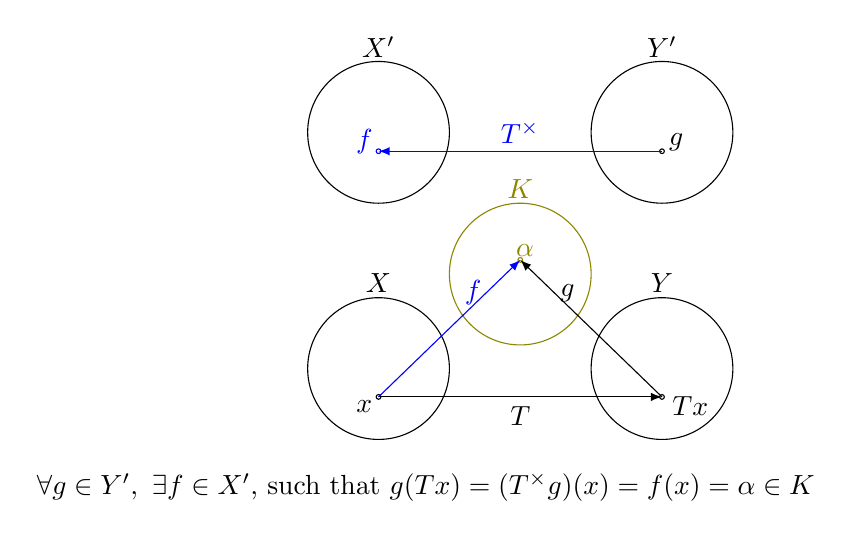
\begin{tikzpicture}[scale=0.6]
	\draw (-3,0) circle (1.5cm);
	\draw (-3,1.8) node{$X$};
	\draw (3,0) circle (1.5cm);
	\draw (3,1.8) node{$Y$};
	\draw (-3,5) circle (1.5cm);
	\draw (-3,6.8) node{$X'$};
	\draw (3,5) circle (1.5cm);
	\draw (3,6.8) node{$Y'$};
	\draw[olive] (0,2.0) circle (1.5cm);
	\draw[olive] (0,3.8) node{$K$};

	\draw (-3,-0.6) circle (0.05cm);
	\draw (-3.3,-0.8) node{$x$};
	\draw (3,-0.6) circle (0.05cm);
	\draw (3.6,-0.8) node{$Tx$};
	\draw[blue] (-3,4.6) circle (0.05cm);
	\draw[blue] (-3.3,4.8) node{$f$};
	\draw (3,4.6) circle (0.05cm);
	\draw (3.3,4.8) node{$g$};
	\draw[olive] (0,2.3) circle (0.05cm);
	\draw[olive] (0.1,2.5) node{$\alpha$};

	\draw[-latex] (3,-0.6) -- (0,2.3);
	\draw (1,1.6) node{$g$};
	\draw[-latex,blue] (-3,-0.6) -- (0,2.3);
	\draw[blue] (-1,1.6) node{$f$};
	\draw[-latex] (-3,-0.6) -- (3,-0.6);
	\draw[blue] (0,5) node{$T^\times$};
	\draw[-latex,blue] (3,4.6) -- (-3,4.6);
	\draw (0,-1) node{$T$};
	\draw (-2,-2.5) node{$\forall g \in Y',\ \exists f \in X'$, such that $g(Tx) = (T^\times g)(x) = f(x) = \alpha \in K$};
\end{tikzpicture}
		\caption{Adjoint-Operator}
\end{figure}
\end{commentary}

\begin{theorem}[norm]
	Let $T^\times$ be the adjoint operator of a bounded, linear operator $T$.
	Then $T^\times$ is a bounded, linear operator.
	And $\|T^\times\| = \|T\|$.
\end{theorem}
\begin{proof}
	Let $g_1,g_2 \in Y'$ and $\alpha,\beta \in K$.
	Then,
	\begin{align*}
		\left(T^\times (\alpha g_1 + \beta g_2) \right)(x)
		& = (\alpha g_1 + \beta g_2) Tx \\
		& = \alpha g_1(Tx) + \beta g_2(Tx) \\
		& = \alpha (T^\times g_1)(x) + \beta (T^\times g_2)(x)
	\end{align*}
	Clearly, $T^\times$ is linear.\\

	We have, $f = T^\times g$.
	\begin{align*}
		f(\alpha x_1 + \beta x_2)
		& = (T^\times g)(\alpha x_1 + \beta x_2) \\
		& = g(T(\alpha x_1 + \beta x_2)) \\
		& = g(\alpha Tx_1 + \beta Tx_2) \\
		& = \alpha g(Tx_1) + \beta g(Tx_2) \\
		& = \alpha (T\times g)x_1 + \beta (T^\times g)x_2 \\
		& = \alpha f(x_1) + \beta f(x_2)
	\end{align*}
	Thus, $f$ is linear.
	We have $|g(Tx)| \le \|g\| \ \|T\| \ \|x\|$, since functional $g$ and operator $T$ are bounded.
	Thus,
	\[ \|T^\times g \| = \|f\| = \sup_{x \ne 0} \frac{|f(x)|}{\|x\|} = \sup_{x \ne 0} \frac{|g(Tx)|}{\|x\|} \le \sup_{x \ne 0} \frac{\|g\| \ \|T\| \ \|x\|}{\|x\|} \le \|g\| \ \|T\| \]
	Taking supermum over all $g \in Y'$, we get
	\[ \|T^\times\| \le \sup_{g \ne 0} \frac{\|T^\times g\|}{\|g\|} = \sup_{g \ne 0} \frac{\|g\| \ \|T\|}{\|g\|} = \|T\| \]
	
	We know that for any non-zero $x_0 \in X$ there exists a $g_0 \in Y'$ such that $\|g_0\| = 1$ and $g_0(Tx_0) = \|Tx_0\|$.
	Let $f_0 = T^\times g_0$.
	Then,
	\[ \|Tx_0\| = g_0(Tx_0) = f_0(x_0) \le \|f_0\| \ \|x_0\| = \|T^\times g_0\| \ \|x_0\| \le \|T^\times\| \ \|g_0\| \ \|x_0\| \]
	Thus, $\|Tx_0\| \le \|T^\times\| \ \|x_0\|$.
	Taking supremum over $x_0$ we get, $\|T\| \le \|T^\times\|$.\\

	We have $\|Tx_0\| \le \|T\|\ \|x_0\|$.
	And $\|T\| = c$ is the smallest real number satisfying $\|Tx_0\| \le c\|x_0\|,\ \forall x_0 \in X$.
	Thus, $\|T^\times\| \ge c$.
	Therefore,
	\[ \|T^\times\| \ge \|T\| \]
	Therefore, $\|T^\times\| = \|T\|$.
\end{proof}

\begin{remark}[Properties of adjoint-operator]
	Let $S : Y \to Z$ and $T : X \to Y$ be bounded, linear operators.
	Let $\alpha \in K$.
	Then,
\begin{enumerate}
	\item If $T_{E}$ is the matrix representation of $T$, then transpose of $T_{E}$ is the matrix representation of $T^\times$.
	\begin{proof}
		Let $T_E$ be the matrix representation of linear operator $T : \mathbb{R}^n \to \mathbb{R}^n$ with respect to standard basis $E = \{ e_1,\ e_2,\ \dots,\ e_n \}$.
		Let $x = (\xi_j)$ and $y = (\eta_j)$.
		Then $y = Tx$ implies $\displaystyle \eta_j = \sum_{k=1}^n \tau_{j,k} \xi_k$.
		Define $T_E = (\tau_{j,k})$.
		Then $y = T_E x$.
		We know that $(\mathbb{R}^n)^\prime = \mathbb{R}^n$.
		Let $g$ be a bounded, linear operator on $\mathbb{R}^n$.
		Then $g \in \mathbb{R}^n$ and $\displaystyle g = \sum_{k = 1}^n \alpha_k f_k$ where $F = \{ f_1,\ f_2,\ \dots,\ f_n\}$ is the dual basis of $E$.
		That is, $f_k(e_j) = \delta_{k,j}$.
		\[ g(y) = g(T_E x) = \sum_{j = 1}^n \alpha_j \eta_j = \sum_{j = 1}^n \sum_{k=1}^n \alpha_j \tau_{j,k}\xi_k \]
		Thus,
		\[ g(T_E x) = \sum_{k=1}^n \beta_k \xi_k \text{ where } \beta_k = \sum_{j=1}^n \tau_{j,k} \alpha_j \]
		Define $f : X \to K$ where $f(x) = g(Tx)$.
		Then,
		\[ f(x) = g(T_E x) = \sum_{k=1}^n \beta_k \xi_k \]
		Suppose $f = T_E^\times g$.
		Then matrix of $T_E^\times$ is given by $(\tau_{j,k})$ since $\displaystyle \beta_k = \sum_{j=1}^n \tau_{j,k} \alpha_j$.
		Thus, matrix of $T^\times$ is the transpose of that of $T_E$.
	\end{proof}
	\item $(S+T)^\times = S^\times + T^\times$
	\begin{proof}
	\begin{align*}
		((S+T)^\times g)(x)
		& = g((S+T)x)  \\
		& = g(Sx + Tx) \\
		& = g(Sx) + g(Tx) \\
		& = (S^\times g)(x) + (T^\times g)(x)
	\end{align*}
	\end{proof}
	\item $(\alpha T)^\times = \alpha T^\times$
	\begin{proof}
	\begin{align*}
		((\alpha T)^\times g)(x)
		& = g((\alpha T)x) \\
		& = g(\alpha Tx) \\
		& = \alpha g(Tx) \\
		& = \alpha (T^\times g)(x)
	\end{align*}
	\end{proof}
	\item $(T^\times)^{-1} = (T^{-1})^\times$\\
		Suppose $T : X \to Y$ is invertible and $T^{-1} : Y \to X$.
		Then $(T^\times)^{-1}$ exists and $(T^\times)^{-1} = (T^{-1})^\times$.
	\begin{proof}
		We have $T \in B(X,Y)$ and $T^\times \in B(Y',X')$.
		Define $S = T^{-1}$.
		Then $S \in B(Y,X)$.
		Thus $S^\times$ exists, since $S$ is a bounded, linear operator.
		And $S^\times \in B(X',Y')$.\\

		Let $g \in Y'$.
		Then,
		\[ g(y) = g(TSy) = (T^\times g)(Sy) = (S^\times T^\times g)(y),\ \forall g \in Y' \]
		Clearly, $T^\times S^\times$ is an identity operator on $Y'$.\\

		Let $f \in X'$.
		Then,
		\[ f(x) = f(STx) = (S^\times f)(Tx) = (T^\times S^\times f)(x),\ \forall f \in X' \]
		Clearly, $S^\times T^\times$ is an identity operator on $X'$.\\

		Therefore, $S^\times = (T^{-1})^\times = (T^\times)^{-1}$.
	\end{proof}
\end{enumerate}
\end{remark}

\begin{figure}
\centering
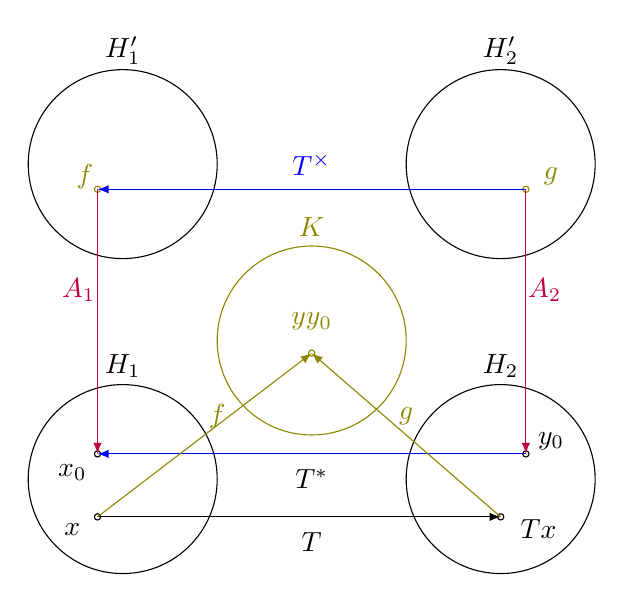
\begin{tikzpicture}[scale=0.8]
	\draw (-3,0) circle (1.5cm);
	\draw (-3,1.8) node{$H_1$};
	\draw (3,0) circle (1.5cm);
	\draw (3,1.8) node{$H_2$};
	\draw (-3,5) circle (1.5cm);
	\draw (-3,6.8) node{$H_1'$};
	\draw (3,5) circle (1.5cm);
	\draw (3,6.8) node{$H_2'$};
	\draw[olive] (0,2.2) circle (1.5cm);
	\draw[olive] (0,4.0) node{$K$};

	\draw (-3.4,-0.6) circle (0.05cm);
	\draw (-3.8,-0.8) node{$x$};
	\draw (3,-0.6) circle (0.05cm);
	\draw (3.6,-0.8) node{$Tx$};
	\draw (-3.4,0.4) circle (0.05cm);
	\draw (-3.8,0.1) node{$x_0$};
	\draw (3.4,0.4) circle (0.05cm);
	\draw (3.8,0.6) node{$y_0$};
	\draw[olive] (-3.4,4.6) circle (0.05cm);
	\draw[olive] (-3.6,4.8) node{$f$};
	\draw[olive] (3.4,4.6) circle (0.05cm);
	\draw[olive] (3.8,4.8) node{$g$};

	\draw[-latex,blue] (3.4,4.6) -- (-3.4,4.6);
	\draw[blue] (0,5) node{$T^\times$};
	\draw[-latex] (-3.4,-0.6) -- (3,-0.6);
	\draw (0,-1) node{$T$};
	\draw[-latex,blue] (3.4,0.4) -- (-3.4,0.4);
	\draw (0,0) node{$T^\ast$};
	\draw[-latex,purple] (3.4,4.6) -- (3.4,0.4);
	\draw[purple] (-3.7,3) node{$A_1$};
	\draw[-latex,purple] (-3.4,4.6) -- (-3.4,0.4);
	\draw[purple] (3.7,3) node{$A_2$};

	\draw[-latex,olive] (3,-0.6) -- (0,2);
	\draw[olive] (1.5,1) node{$g$};
	\draw[olive] (0,2) circle (0.05cm);
	\draw[olive] (0,2.5) node{$\inner{y}{y_0}$};
	\draw[-latex,olive] (-3.4,-0.6) -- (0,2);
	\draw[olive] (-1.5,1) node{$f$};
\end{tikzpicture}
\caption{Adjoint-Operator vs Hilbert-Adjoint-Operator}
\end{figure}

\begin{remark}[$T^\times$ vs $T^\ast$]
	Let $T : H_1 \to H_2$.
	Let $T^\times$ be the adjoint-operator of $T$.
	That is, $T^\times : H_2' \to H_1'$.
	Let $T^\ast : H_2 \to H_1$ be the Hilbert-adjoint operator of $T$.
	That is, $\inner{Tx}{y} = \inner{x}{T^\ast y}$.
	Then,
	\[ T^\ast = A_1 T^\times A_2^{-1} \]
	where $A_1 : H_1' \to H_1$ defined by $A_1(f) = x_0$ such that $f(x) = \inner{x}{x_0}$ and $A_2 : H_2' \to H_2$ defined by $A_2(g) = y_0$ such that $g(y) = \inner{y}{y_0}$.

\end{remark}
\begin{proof}
	Let $H_1,H_2$ be normed spaces.
	Let $T : H_1 \to H_2$ be a bounded, linear operator.
	Then there exists unique adjoint operator $T^\times : H_2' \to H_1'$ defined by $(T^\times g)(x) = g(Tx),\ \forall g \in Y',\ \forall x \in H_1$.
	And there exists unique Hilbert adjoint operator $T^\ast : H_2 \to H_1$ defined by $\inner{Tx}{y} = \inner{x}{T^\ast y},\ \forall x \in H_1,\ \forall y \in H_2$.\\

	Let $f \in H_1'$.
	By Riesz theorem, $\forall f \in H_1'$ there exists unique $x_0 \in H_1$ such that $f(x) = \inner{x}{x_0}$.
	Define $A_1 : H_1' \to H_1$ defined by $A_1(f) = x_0$ where $f(x) = \inner{x}{x_0},\ \forall x \in H_1$.
	Clearly, $A_1$ is bijective by its construction.
	Let $g \in H_2'$.
	By Riesz theorem, $\forall g \in H_2'$, there exists unique $y_0 \in H_2$ such that $g(y) = \inner{y}{y_0}$.
	Define $A_2 : H_2' \to H_2$ defined by $A_2(g) = y_0$ where $g(y) = \inner{y}{y_0},\ \forall y \in H_2$.
	Clearly, $A_2$ is bijective by its construction.\\

	Let $A_1(f_1) = x_1$ and $A_1(f_2) = x_2$.
	Then, we have $f_1(x) = \inner{x}{x_1}$ and $f_2(x) = \inner{x}{x_2}$.
	Thus,
	\begin{align*}
		(\alpha f_1 + \beta f_2))(x)
		& = \alpha f_1(x) + \beta f_2(x) \\
		& = \alpha \inner{x}{x_1} + \beta \inner{x}{x_2} \\
		& = \inner{x}{\conj{\alpha}x_1} + \inner{x}{\conj{\beta}x_2} \\
		& = \inner{x}{\conj{\alpha}x_1+\conj{\beta}x_2}\\
		A_1(\alpha f_1+\beta f_2) & = \conj{\alpha} x_1 + \conj{\beta}x_2 \\
		& = \conj{\alpha}A_1(f_1) + \conj{\beta}A_1(f_2)
	\end{align*}
	Thus, $A_1$ is conjugate linear.
	Similarly, $A_2$ is also conjugate linear.\\

	Let $S = A_1 T^\times A_2^{-1}$.
	Let $A_1(f) = x_0$ and $A_2(g) = y_0$.
	Then $S : H_2 \to H_1$ defined by $S(y_0) = (A_1 T^\times A_2^{-1})(y_0) = (A_1 T^\times) (g)  = A_1(f) = x_0$.
	And $S$ is linear since $A_1$ and $A_2^{-1}$ are conjugate linear.
	Then,
	\[ \inner{Tx}{y_0} = g(Tx) = f(x) = \inner{x}{x_0} =  \inner{x}{S y_0} \]
	But, we have, $\inner{Tx}{y_0} = \inner{x}{T^\ast y_0}$.
	And we know that, $w_1 = w_2$ if $\inner{v}{w_1} = \inner{v}{w_2}, \forall v$.
	Thus, $S = T^\ast = A_1 T^\times A_2^{-1}$.
\end{proof}

\begin{remark}Comparison
\begin{enumerate}
	\item Matrix of adjoint operator is transpose. But, matrix of Hilbert adjoint operator is complex conjugate transpose.
	\item Adjoint operator is linear, but Hilbert-adjoint operator is conjugate linear.
\end{enumerate}
\end{remark}

\subsection{Exercises}
\cite[\S 4.5 Exercise 6]{kreyszig}
\begin{remark}
	\[ (T^\times)^n = (T^n)^\times \]
\end{remark}
\begin{proof}
	Let $T : X \to X$ be a bounded, linear operator.
	\[ g(T^2 x) = g(T(Tx)) = (T^\times g)(Tx) = T^\times T^\times g(x) = (T^\times)^2 g(x) \]
	Suppose $(T^\times)^{k-1} = (T^{k-1})^\times$ for some $k \in \mathbb{N}$.
	Then,
	\[ g(T^k x) = g(T(T^{k-1}x)) = (T^\times g)(T^{k-1}x) = T^\times (T^\times)^{k-1} g(x) = (T^\times)^k g(x) \]
	Therefore, by finite mathematical induction the result is true.
\end{proof}

\begin{definition}[Annihilator in a normed space]
	Let $X$ be a normed space and $M$ be a subset of $X$.
	Then the annihilator of $M$ is given by,
	\[ M^a = \left\{ f \in X^\prime : f(M) = \{ 0 \} \right\} \]
\end{definition}

\begin{definition}[Annihilator in a dual space]
	Let $X$ be a normed space and $X^\prime$ be its dual space.
	Let $B$ be a subset of $X^\prime$.
	Then the annihilator of $B$ is given by,
	\[ \hphantom{x}^aB = \{ x \in X : f(x) = 0,\ \forall f \in B \} \] %\sideset{^a}{}B$ not working
\end{definition}

\begin{remark}
	\[ \mathscr{R}(T) \subset \hphantom{x}^a\mathcal{N}(T^\times) \]
\end{remark}
\begin{proof}
	Let $T : X \to Y$ be a bounded, linear operator.
	Let $f \in \mathcal{N}(T^\times)$.
	Then $T^\times f = 0$.
	Let $y = Tx \in \mathscr{R}(T)$.
	Then,
	\[ f(y) = f(Tx) = (T^\times f) (x) = 0,\ \forall y \in \mathscr{R}(T) \]
	Thus, $y \in \mathscr{R}(T) \implies y \in \hphantom{x}^a\mathcal{N}(T^\times)$.
\end{proof}

%\subsection{Reflexive Spaces}
%\subsection{Category Theory, Uniform boundedness Theorem}
